\chapter{Particle ID in ND-GAr}
\label{chapter:garsoft_pid}

% more on ND-GAr and the ND, and why we want to do this!
ND-GAr is a magnetised, high-pressure gaseous argon TPC (HPgTPC), surrounded by an electromagnetic calorimeter (ECal) and a muon detector (commonly refer to as $\mu$ID). A detailed discussion on the requirements, design, performance and physics of ND-GAr can be found in the DUNE ND CDR \cite{DUNE2021NDCDR} and the ND-GAr whitepaper (cite).

In DUNE Phase II ND-GAr will fulfill the role of TMS, measuring the momentum and sign of the charged particles exiting ND-LAr. Additionally, it will be able to measure neutrino interactions inside the HPgTPC, achieving lower energy thresholds than those of the ND and FD LArTPCs. By doing so ND-GAr will allow to constrain the relevant systematic uncertainties for the LBL analysis even further.

The goal of the present chapter is to review the requirements that the physics program of DUNE impose on ND-GAr, present the current status of its design and describe the GArSoft package, its simulation and reconstruction software.

As decided during the DUNE Phase II workshop in June 2023 [reference], we want to build ND-GAr physics case by showing:
\begin{itemize}
    \item That ND-GAr can constrain systematic uncertainties that ND-LAr might miss.
    \item The impact on the neutrino oscillation results if such systematic uncertainties are missed.
    \item That ND-GAr is necessary to reach DUNE's main physics goals.
\end{itemize}

This way, the design of ND-GAr will be physics driven.

In order to study the effects of final state interactions (FSI) in CC interactions, ND-GAr should be able to measure the spectrum of protons and charged pions at low energies. ND-GAr also needs to be able to measure the pion multiplicity, specially for energies above $100~\mathrm{MeV}$ as at these energies the pions shower in the LAr, to inform the pion mass correction in the ND and FD LArTPCs.

In order to correctly identify electrons, muons, pions, kaons and protons ND-GAr can use a combination of: $\mathrm{d}E/\mathrm{d}x$ measurements in the HPgTPC, $E_{ECAL}/p$ using the ECAL total energy and the momentum obtained from magnetic spectroscopy in the HPgTPC and penetration information through the ECAL and muon tagger.

\section{GArSoft}\label{section:garsoft}

GArSoft is a software package developed for the simulation and reconstruction of events in ND-GAr. It is inspired by the LArSoft toolkit used for the simulation of LArTPC experiments, like the DUNE FD modules. It is based on \texttt{art}, the framework for event processing in particle physics experiments \cite{ART}. Other of its main dependencies are \texttt{ROOT}, \texttt{NuTools}, \texttt{GENIE} and \texttt{Geant4}. It allows the user to run all the steps of a generation-simulation-reconstruction workflow using FHiCL configuration files.

\subsection{Event generation}

The standard generator FHiCLs in GArSoft run the event generation and particle propagation simulation (i.e. Geant4) in the same job by default. However, it is possible to split them up if needed. The current version of GArSoft provides five different event generators, each of them producing \texttt{simb::MCTruth} products defined in \texttt{NuTools}. The available modules are:
\begin{itemize}
	\item \texttt{SingleGen}: particle gun generator. It produces the specified particles with a given distribution of momenta, initial positions and angles.
	\item \texttt{TextGen}: text file generator. The input file must follow the \texttt{hepevt} format\footnote{In brief, each event contains at least two  lines.  The first line contains two entries, the event number and the number of particles in the event. Each following line contains 15 entries to describe each particle. The entries are: status code, pdg code for the particle, entry of the first mother for this particle, entry of the second mother for this particle, entry of the first daughter for this particle, entry of the second daughter for this particle, x component of the particle momentum, y component of the particle momentum, z component of the particle momentum, energy of the particle, mass of the particle, x component of the particle initial position, y component of the particle initial position, z component of the particle initial position and time of the particle production.}, the module simply copies this to \texttt{simb::MCTruth} data products.
	\item \texttt{GENIEGen}: GENIE neutrino event generator. The module runs the neutrino-nucleus interaction generator using the options specified in the driver FHiCL file (flux file, flavour composition, number of interactions per event, $t_{0}$ distribution, ...). Current default version is \texttt{v3_04_00}.
	\item \texttt{RadioGen}: radiological generator. It produces a set list of particles to model radiological decays. Not tested.
	\item \texttt{CRYGen}: cosmic ray generator. The module runs the CRY event generator with a configuration specified in the FHiCL file (latitude and altitude of detector, energy threshold, ...). Not tested.
\end{itemize}

The module \texttt{GArG4} searches for all the generated \texttt{simb::MCTruth} data products, using them as inputs to the Geant4 simulation with the specified detector geometry. A constant $0.5~\mathrm{T}$ magnetic field along the drift coordinate is assumed. The main outputs of this step are \texttt{simb::MCParticle} objects for the generated Geant4 particles, \texttt{gar::EnergyDeposit} data products for the energy deposits in the HPgTPC and \texttt{gar::CaloDeposit} data products for the energy deposits in the ECal and muon system.

\subsection{Detector simulation}

The standard detector simulation step in GArSoft is all run with a single FHiCL, but the different modules can be run independently as well. First the \texttt{IonizationReadout} module simulates the charge readout of the HPgTPC, and later the \texttt{SiPMReadout} module runs twice, once for the ECal and then for the muon system, with different configurations.

The \texttt{IonizationAndScintillation} module collects all the \texttt{gar::EnergyDeposit} data products, to compute the equivalent number of ionization electrons for each energy deposit. The \texttt{ElectronDriftAlg} module simulates the electron diffusion numerically both in the longitudinal and transverse directions and applies an electron lifetime correction factor. The induced charge on the nearest and neighbouring readout pads is modeled using the provided pad response functions. The digitisation of the data is then simulated with the \texttt{TPCReadoutSimAlg} module. By default, the ADC sampling rate used is $50.505~\mathrm{MHz}$. The resulting raw waveforms for each channel are stored with zero-suppression, in order to save memory and CPU time. The algorithms keep blocks of ADC values above a certain threshold, plus some adjustable additional early and late tick counts. The results of these three steps are \texttt{gar::raw::RawDigit} data products.

For the ECal and the muon system the \texttt{SiPMReadout} module calls either the \texttt{ECALReadoutSimStandardAlg} or \texttt{MuIDReadoutSimStandardAlg} modules. These take all the \texttt{gar::CaloDeposit} data products in the corresponding detector and do the digitisation depending on whether the hit was in a tile or strip layer. They include single photon statistics, electronic noise, SiPM saturation and time smearing. The resulting objects are \texttt{gar::raw::CaloRawDigit} data products.

\subsection{Reconstruction}

The reconstruction in GArSoft is also run as a single job by default. It first runs the hit finding, clustering, track fitting and vertex identification in the HPgTPC, followed by the hit finding and clustering in the ECal and muon system. After those it produces the associations between the associations between the tracks and the ECal clusters.

Focusing first on the HPgTPC reconstruction, the \texttt{CompressedHitFinder} module takes the zero-suppressed ADCs from the \texttt{gar::raw::RawDigit} data products. The reconstructed hits largely correspond to the above threshold blocks, however the hit finder identifies waveforms with more than one maximum, diving them in multiple hits if they dip below a certain threshold. The data products produced are of the form \texttt{gar::rec::Hit}. These are the inputs to the clustering of hits in the \texttt{TPCHitCluster} module. Hits close in space and time are merged, and the resulting centroids are found. This module outputs \texttt{gar::rec::TPCClusters} objects and associations to the input hits.

The following step prior to the track fitting is pattern recognition. The module called \texttt{tpcvechitfinder2} uses the \texttt{gar::rec::TPCClusters} data products to find track segments, typically called vector hits. They are identified by performing linear 2D fits to the positions of the clusters in a $10~\mathrm{cm}$ radius, one fit for each coordinate pair. A 3D fit defines the line segment of the vector hit, using as independent variable the one whose sum of (absolute value) slopes in the 2D fits is the smallest. The clusters are merged to a given vector hit if they are less than $2~\mathrm{cm}$ away from the line segment. The outputs are \texttt{gar::rec::VecHit} data products, as well as associations to the clusters. The \texttt{tpcpatrec2} module takes the \texttt{gar::rec::VecHit} objects to form the track candidates. The vector hits are merged together if their direction matches, their centers are within $60~\mathrm{cm}$ and their direction vectors point roughly to their respective centers. Once the clusters of vector hits are formed they are used to make a first estimation of the track parameters, simply taking three clusters along the track. The module produces \texttt{gar::rec::Track} data products and associations between these tracks and the clusters and vector hits.

The track is fitted by means of a Kalman filter in the \texttt{tpctrackfit2} module, using the position along the drift direction as the independent variable. Two different fits are performed per track, a forward and a backwards fit, each starting from one of the track ends. The Kalman filter state vector $(y,z,R,\phi,\mathrm{tan}\lambda)$ is estimated at each point along the track using a Bayesian update. The track parameters reported in the forward and backwards fits are the ones computed at the opposite end where the fit started. The main outputs of the track fit are the \texttt{gar::rec::Track} objects. Additionally, the module stores the fitted 3D positions along the track in the \texttt{gar::rec::TrackTrajectory} data products and the total charge and step sizes for each point also get stored in the form of \texttt{gar::rec::TrackIonization} objects.

\begin{figure}[t]
	\centering
	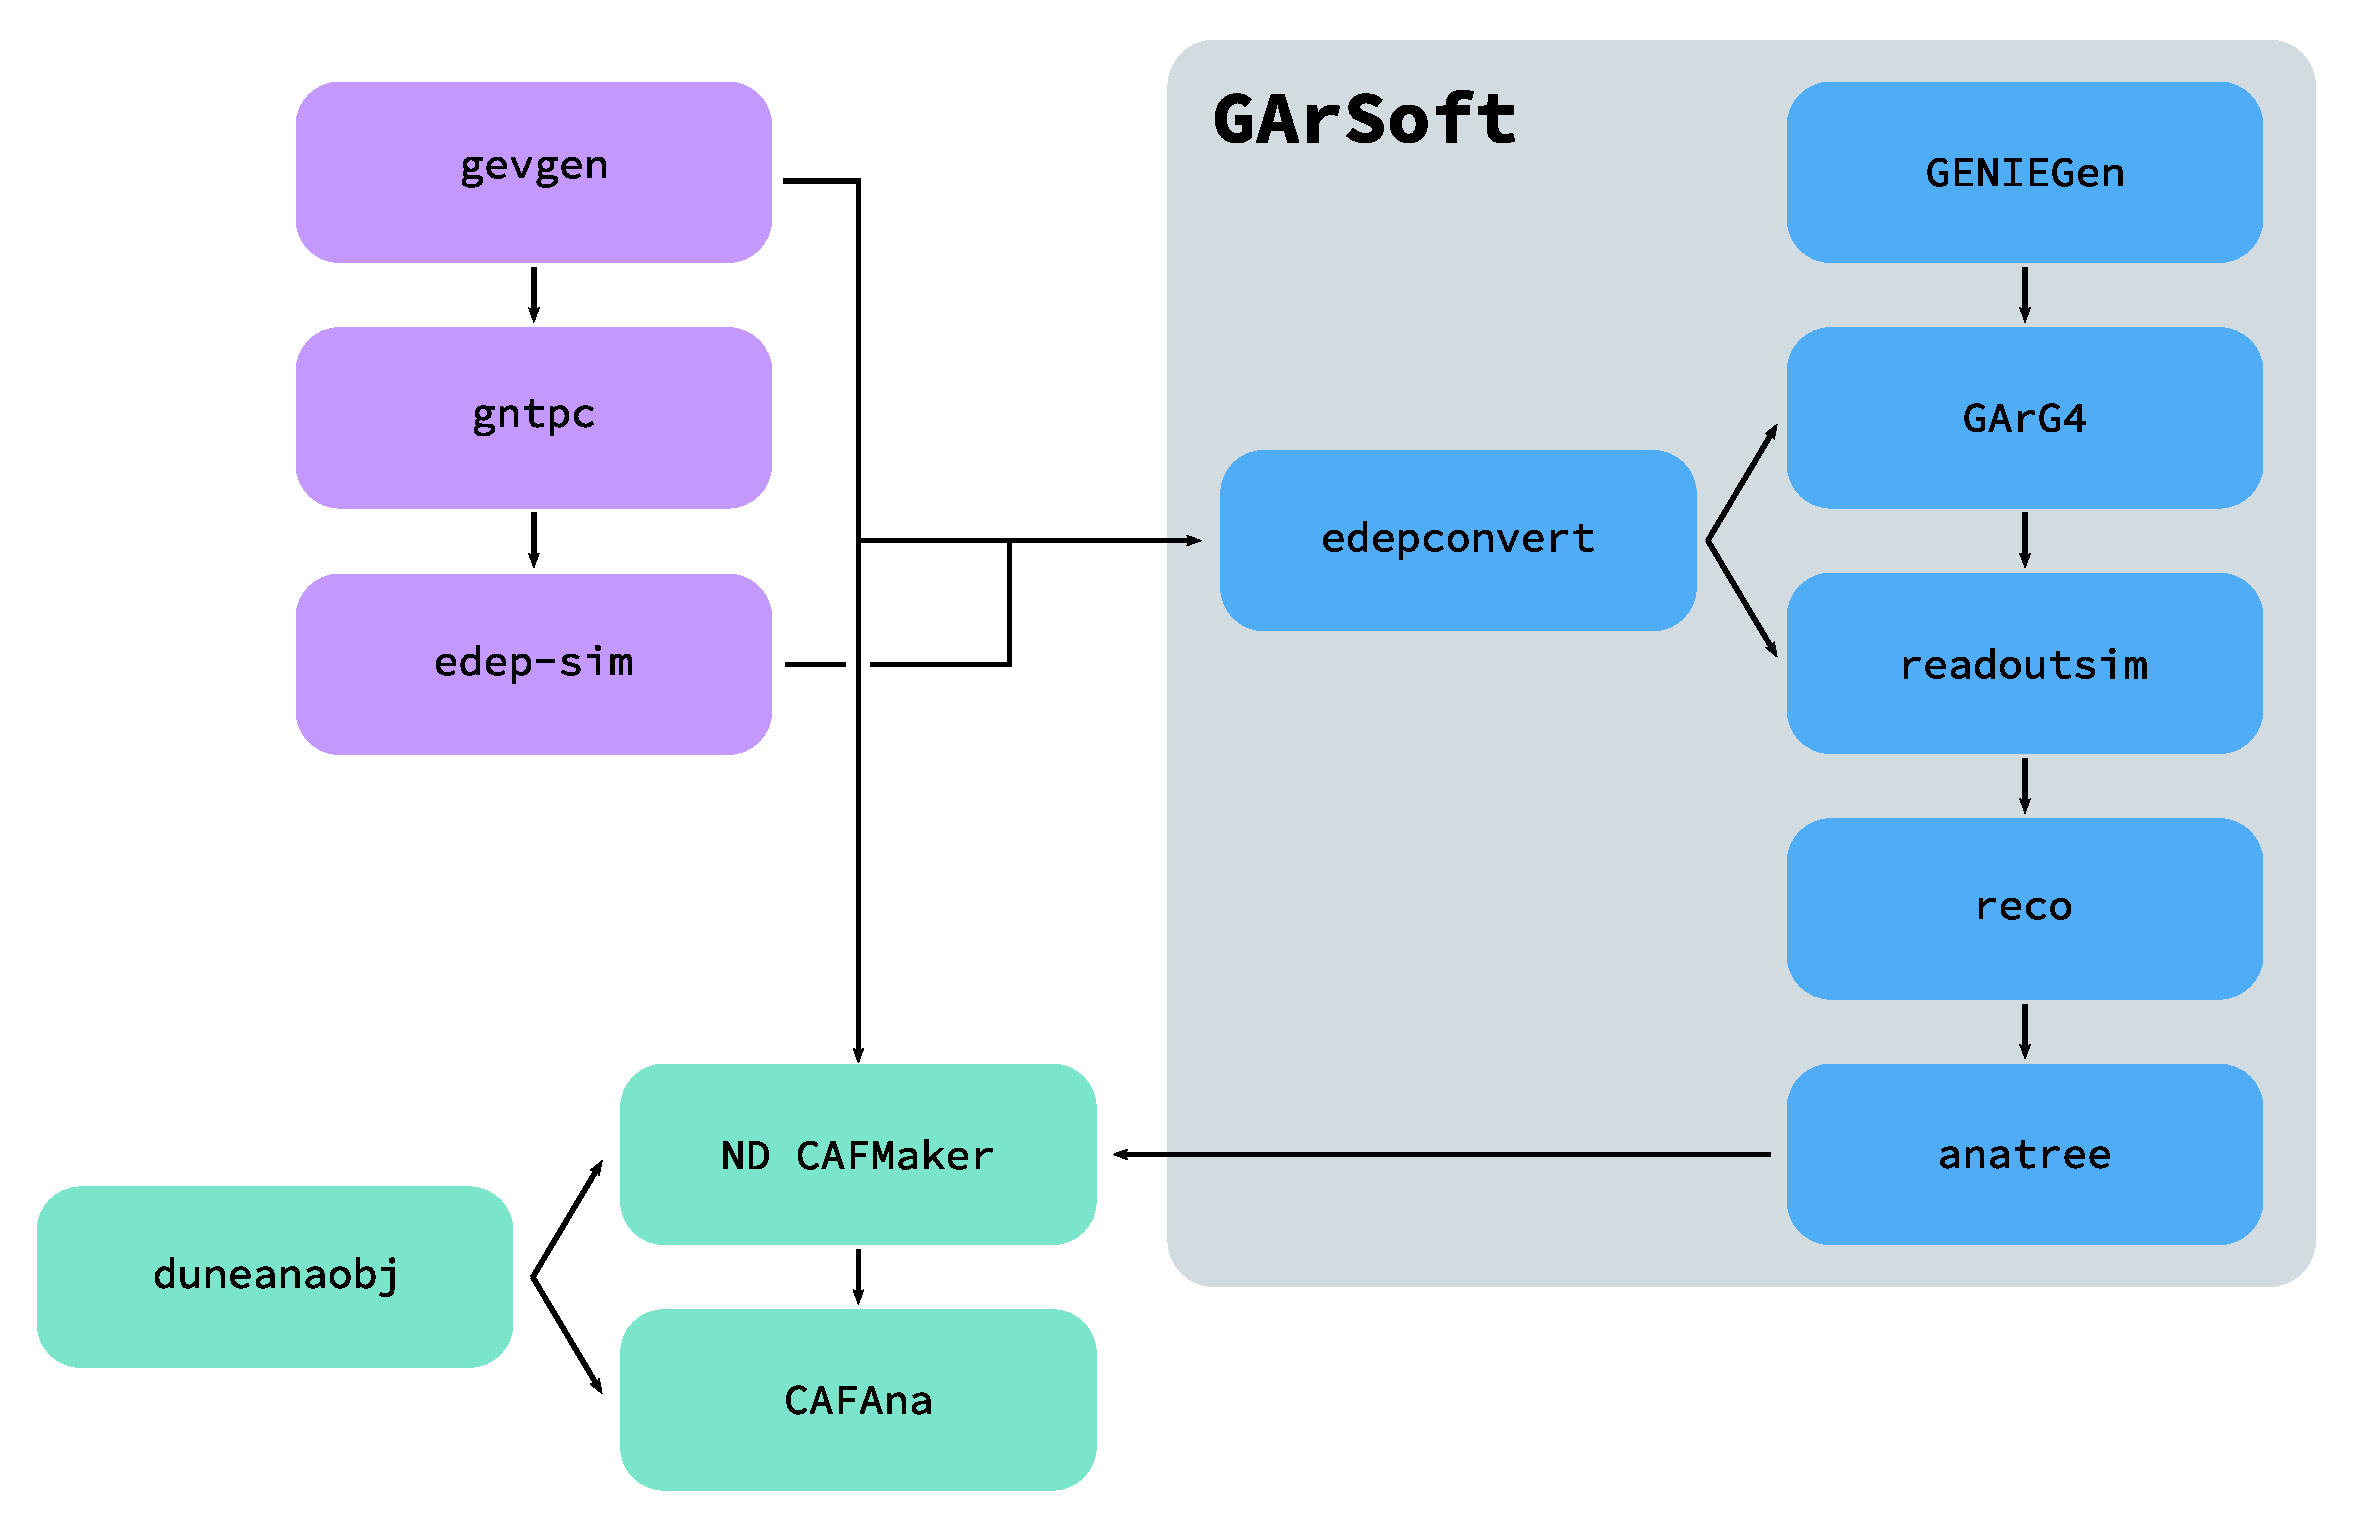
\includegraphics[width=.90\linewidth]{Images/GArSoft_PID/gar_workflow.pdf}
	\caption{Schematic diagram showing the different modules involved in the ND-GAr production.}
	\label{fig:gar_workflow}
\end{figure}

After the tracking step, the \texttt{vertexfinder1} module looks at the reconstructed \texttt{gar::rec::Track} products, creating vertex candidates with the track ends that are within $12~\mathrm{cm}$ of each other. The vertices are then fitted using linear extrapolations from the different track ends associated. The results are \texttt{gar::rec::Vertex} data products, and associations to the tracks and corresponding track ends.

For the ECal and muon tagger, the \texttt{SiPMHitFinder} module runs twice with different configurations, adapted to the particular capabilities of both. The module simply takes the \texttt{gar::raw::CaloRawDigit} products, applies a calibration factor to convert the ADC counts to $\mathrm{MeV}$ and for the strip layer hits it calculates the position along the strip using the times recorded of both SiPMs. This module produces \texttt{gar::rec::CaloHit} data products. Next, these objects are used as inputs to the \texttt{CaloClustering} module. It merges the hits based on a simple nearest neighbours (NN) algorithm. For the resulting clusters it also computes the total energy and position of the centroid. The results are stored as \texttt{gar::rec::Cluster} data products, with associations to the hits.

The last step in the reconstruction is associating the reconstructed tracks in the HPgTPC to the clusters formed in the ECal and muon system. The \texttt{TPCECALAssociation} module checks first the position of the track end points, considering only the points that are at least $215~\mathrm{cm}$ away from the cathode or have a radial distance to the center greater than $230~\mathrm{cm}$. The candidates are propagated up to the radial position, in the case of clusters in the barrel, or the drift coordinate position, for the end cap cluster, of the different clusters in the collection using the track parameters computed at the end point. The end point is associated to the cluster if certain proximity criteria are met. This module creates associations between the tracks, the end points and the clusters. The criteria for the associations are slightly different for the ECal and the muon tagger.

\section[\texorpdfstring{$\mathrm{d}E/\mathrm{d}x$}{dE/dx} measurement in the TPC]{\boldmath\texorpdfstring{$\mathrm{d}E/\mathrm{d}x$}{dE/dx} measurement in the TPC}\label{section:dEdx}

Among the parameters extracted from the track fitting, ionisation is particularly useful for particle identification, as it is a function of the particle velocity. Although for the case of relativistic particles this dependence is not very strong, measuring the track on a large number of points may allow us to estimate the amount of ionisation accuratel. This, paired with a measurement of the momentum, may allow us to identify the particle type.

The first calculation of the energy loss per unit length of relativistic particles using a quantum-mechanical treatment is due to Bethe \cite{Bethe1930}. Using this approach, the mean ionisation rate of a charged particle traveling through a material medium is (using natural units $G=\hbar=c=1$):
\begin{equation}\label{Eq:3.1}
    \expval{\frac{\mathrm{d}E}{\mathrm{d}x}} = \frac{4 \pi N e^{4}}{m_{e}\beta^{2}} z^{2} \left(\mathrm{log} \frac{2m_{e}\beta^{2}\gamma^{2}}{I} - \beta^{2}\right),
\end{equation}
where $N$ is the number density of electrons in the medium, $e$ the elementary charge, $m_{e}$ is the electron mass, $z$ the charge of the particle in units of $e$, $\beta$ is the velocity of the particle, $\gamma = (1-\beta^{2})^{-1}$ and $I$ denotes the effective ionisation potential averaged over all electrons. This relation is known as the Bethe-Bloch formula.

From Eq. (\ref{Eq:3.1}) one can see that the ionisation loss does not depend explicitly on the mass of the charged particle, that for non-relativistic velocities it falls as $\beta^{-2}$, then goes through a minimum and increases as the logarithm of $\gamma$. This behaviour at high velocities is commonly known as the relativistic rise. The physical origin of this effect is partly due to the fact that the transverse electromagnetic field of the particle is proportional to $\gamma$, therefore as it increases so does the cross section.

It was later understood that the relativistic rise could not grow indefinitely with $\gamma$. A way to add this feature in the Bethe-Bloch formula is by introducing the so-called density effect term. It accounts for the polarisation effect of the atoms in the medium, which effectively shield the electromagnetic field of the charged particle halting any further increase of the energy loss \cite{Fermi1940}. Denoting the correction as $\delta(\beta)$, one can rewrite Eq. (\ref{Eq:3.1}) as:
\begin{equation}\label{Eq:3.2}
    \expval{\frac{\mathrm{d}E}{\mathrm{d}x}} = \frac{4 \pi N e^{4}}{m_{e}\beta^{2}} z^{2} \left(\mathrm{log} \frac{2m_{e}\beta^{2}\gamma^{2}}{I} - \beta^{2}-\frac{\delta(\beta)}{2}\right).
\end{equation}

In general, the form of $\delta(\beta)$ depends on the medium and its state of aggregation, involving the usage of tabulated parameters and implicit relations \cite{Sternheimer1984}.

Another standard method to compute the amount of ionisation a charged particle produces is the so-called photo-absorption ionisation (PAI) model proposed by Allison and Cobb \cite{Allison1980}. Within their approach, the mean ionisation is evaluated using a semiclassical calculation in which one characterises the continuum material medium by means of a complex dielectric constant $\varepsilon(k, \omega)$. However, in order to model the dielectric constant they rely on the quantum-mechanical picture of photon absorption and collision. Therefore, in the PAI model the computation of the ionisation loss involves a numerical integration of the measured photo-absorption cross-section for the relevant material.

In a particle physics experiment, the typical way of determining the energy loss per unit length as a function of the particle velocity is studying identified particles over a range of momenta. Once we have established this relation we can use it for other, unknown particles. In this sense, it makes sense to have a regular mathematical expression for this relation that one can use.

It happens that neither the Bethe-Bloch theory nor the PAI model from Allison and Cobb offer a close mathematical form for the ionisation curve. This is the reason why a full parametrisation of the ionisation curves can be useful. A parametrisation originally proposed for the \gls{aleph} TPC \cite{Blum2008} and later used by the ALICE TPC \cite{ALICETPC2013} group that manages to capture the features of the ionisation energy loss is:
\begin{equation}\label{Eq:3.3}
    f(\beta\gamma) = \frac{P_{1}}{\beta^{P_{4}}}\left(P_{2}-\beta^{P_{4}}-\mathrm{log}\left[P_{3}+\frac{1}{(\beta\gamma)^{P_{5}}}\right]\right),
\end{equation}
where $P_{i}$ are five free parameters. Hereafter, we will refer to Eq. (\ref{Eq:3.3}) as the \gls{aleph} $\mathrm{d}E/\mathrm{d}x$ parametrisation.

\subsection{Energy calibration}

In order to obtain the amount of energy loss by a charged particle due to ionisation in our TPC we need to determine the conversion between the charge deposited in our readout planes and the actual energy depositions. This procedure is known as energy calibration.

In a general, the first step of the calibration involves a non-uniformity correction, to make sure that the detector response is uniform throughout the TPC. These are typically divided into three categories, non-uniformities in the transverse $YZ$ plane, non-uniformities along the drift direction $X$ and variations of the detector response over time (would not apply to us as the detector is not built yet). These would correct for effects such as electron diffusion and attenuation, space charge effects or channel misconfiguration. However, because at the moment I am only interested in making sure we recover a sensible result from our simulation, I will not apply uniformity corrections to our charge deposits.

Other effects, like electron-ion recombination or ADC saturation, lead to a non-linear relation between the observed charge and the deposited energy in the detector, with the observed readout charge saturating at high ionisation energies. In this case, because we are dealing with gaseous argon and therefore recombination is not as important as in liquid, we do not simulate recombination effects in the TPC. Even so, the simulation of the electronic response will still introduce charge saturation, and one needs to correct for it in order to obtain the exact amount of energy loss due to ionisation.

By default, the track fitting algorithm in GArSoft provides a \texttt{TrackIonization} object associated to each reconstructed track. It contains two collections of charge deposits, one for each fitting direction, consisting on pairs of charge values ($\mathrm{d}Q$, in $\mathrm{ADC}$) and step sizes ($\mathrm{d}x$, in $\mathrm{cm}$).

In order to estimate the ionisation loss in the ND-GAr TPC, I have used an MC sample consisting of single, isotropic protons propagating in the TPC. The starting points of the protons were sampled inside a $50\times50\times25 \ \mathrm{cm}$ box centered at $(100, -150, 1250)$, and their momenta are uniformly distributed in the range $0.25 - 1.75 \ \mathrm{GeV}$. I ran the simulated sample through GArSoft's default detector simulation and reconstruction, and then a custom analyser module that extracts the ionisation data together with other reconstructed track information from the Kalman fit.

\begin{figure}[t]
	\centering
	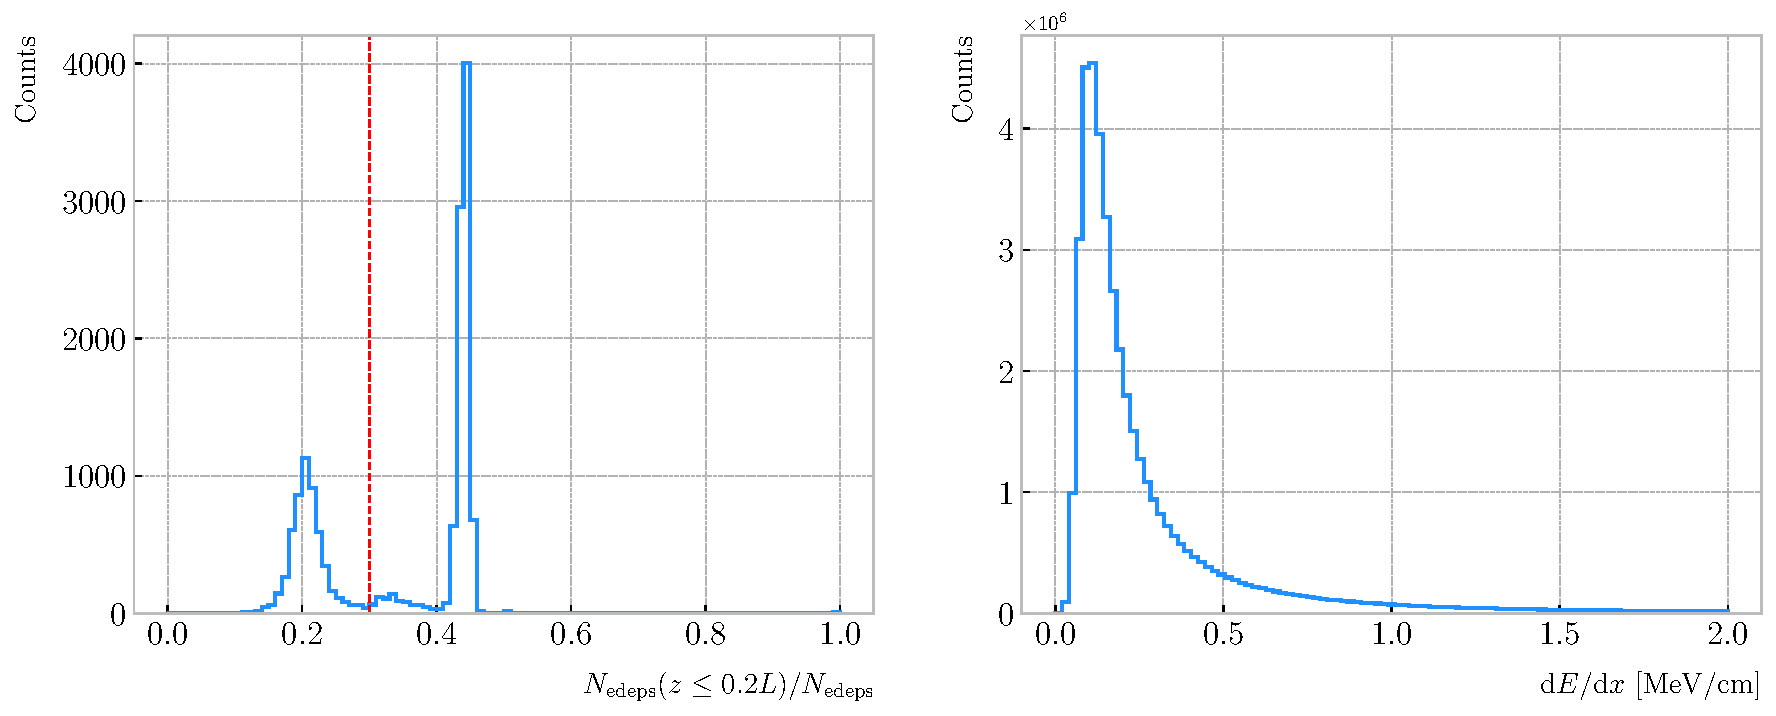
\includegraphics[width=.99\linewidth]{Images/GArSoft_PID/dEdx/geant_selection_dEdx.pdf}
	\caption[Distribution of the fraction of energy deposits with residual range less than $20\%$ of the total track length, and distribution of the ionisation per unit length after removing the tracks with less than $30\%$ of their energy deposits in the last $20\%$ of the track.]{Left panel: distribution of the fraction of Geant4-level energy deposits per track with residual range less than $20\%$ of the total track length, for the isotropic proton sample. Right panel: distribution of the ionisation per unit length of the energy deposits in the proton sample after removing the tracks with less than $30\%$ of their energy deposits in the last $20\%$ of the track.}
	\label{fig:geant_edeps}
\end{figure}

For studying the energy loss of the protons I select the reconstructed tracks that range out (i.e. slow down to rest) inside the TPC. A characteristic feature of the energy loss profile of any stopping ionising particle is the so-called Bragg peak, a pronounced peak that occurs immediately before the particle comes to rest. From Eq. (\ref{Eq:3.1}) we can see that this behaviour is expected, as the energy loss for non-relativistic particles is inversely proportional to $\beta^{2}$. In data, a way of identifying the Bragg peak, and thus select the stopping particles, is checking the number of energy deposits towards the end of the track. In this case, I count the fraction of the Geant4 simulated energy deposits with a residual range value (the distance from a given energy deposit to the last deposit in the track trajectory) less than a $20\%$ of the corresponding track length\footnote{As we are applying this selection at the Geant4 level we could have simply selected the stopping protons using the \texttt{EndProcess} labels from the simulation. However, the Bragg peak identification method displayed here could serve as a starting point for a selection of stopping protons in real data.}. The distribution of this fraction of energy deposits for our proton sample is shown in Fig. \ref{fig:geant_edeps} (left panel). We can clearly see two well separated peaks in this distribution, one centered at $0.2$ and another, narrower, one centered at a higher value. The first one corresponds to non-stopping protons, as in that case the number of energy deposits towards the end of the track is uniformly distributed due to the absence of the Bragg peak. In that way, I apply a cut in this distribution, requiring that at least $30\%$ of the simulated energy deposits sit in the last $20\%$ of the tracks, to ensure that the Bragg peak is present.

\begin{figure}[t]
	\begin{subfigure}{0.5\textwidth}
		\centering
		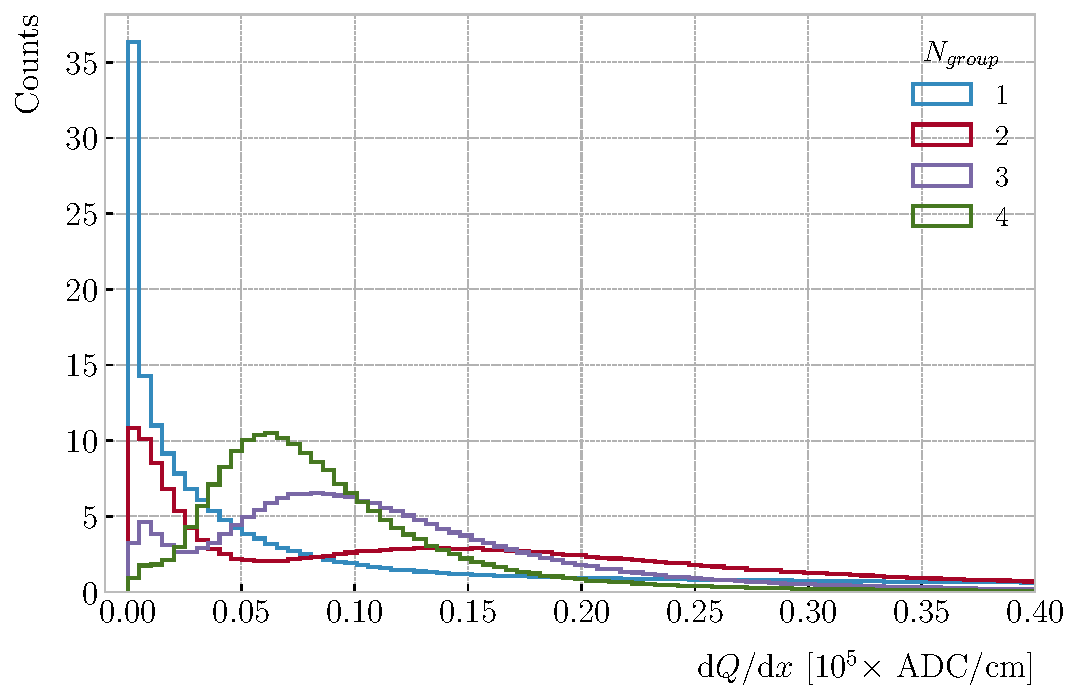
\includegraphics[width=.90\linewidth]{Images/GArSoft_PID/dEdx/reco_dQdx_groups.pdf}
	\end{subfigure}
	\begin{subfigure}{0.5\textwidth}
		\centering
		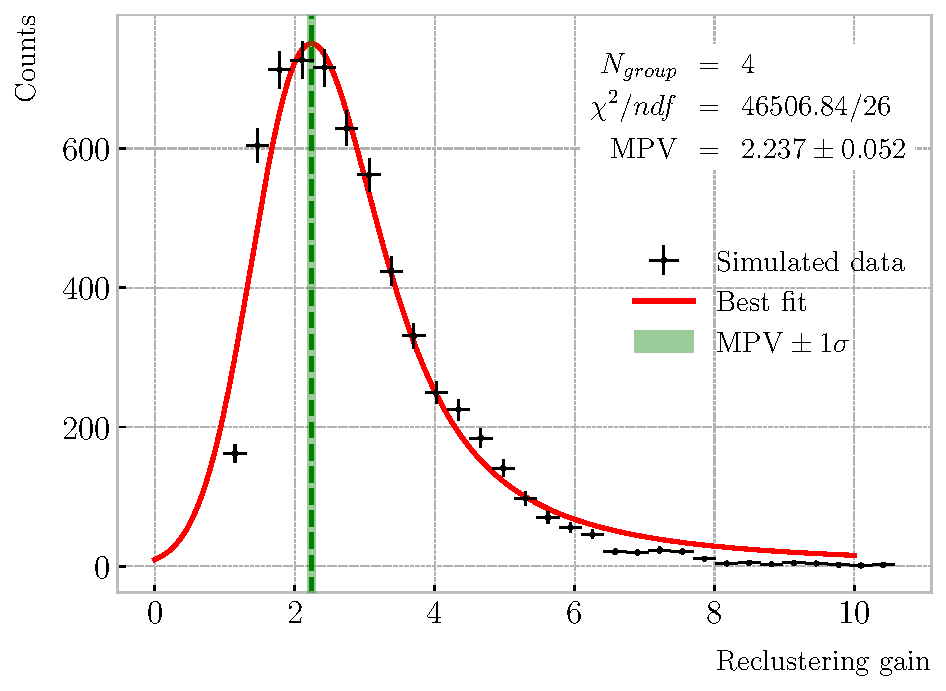
\includegraphics[width=.90\linewidth]{Images/GArSoft_PID/dEdx/dQdx_recluster_gain.pdf}
	\end{subfigure}
	\caption[Distribution of the reconstructed ionisation charge per unit length for different reclustering values, and distribution of the median change in $\mathrm{d}Q/\mathrm{d}x$ per track for the $N_{group}=4$ reclustering.]{Left panel: distribution of the reconstructed ionisation charge per unit length for our MC stopping proton sample. The different colors indicate how many consecutive $\mathrm{d}Q/\mathrm{d}x$ pairs were grouped together. Right panel: distribution of the median change in $\mathrm{d}Q/\mathrm{d}x$ per track after $N_{group}=4$ clusters were reclustered together.}
	\label{fig:reco_dQ_groups}
\end{figure}

Figure \ref{fig:geant_edeps} (right panel) shows the distribution of the energy loss per unit length for the Geant4 simulated energy deposits of the selected stopping protons. We can see that it follows the expected shape of a Landau distribution, which describes the fluctuations of the ionisation energy losses \cite{Landau1944}. This distribution has a characteristic asymmetric PDF, with a long right tail that translates into a high probability for high-energy ionisation losses. The origin of these fluctuations is mainly the possibility of transferring a high enough energy to an electron, so it becomes a ionising particle itself.

Now, from the point of view of the reconstruction, the objects that we have available to extract the ionisation information for the different reconstructed tracks are the collections of $\mathrm{d}Q$ and $\mathrm{d}x$ pairs, as stated before. The $\mathrm{d}Q$ values come from adding up the amplitude of all the reconstructed hits in a cluster, which is the input object to the Kalman fit.

Figure \ref{fig:reco_dQ_groups} (left panel) shows the distribution of the ionisation charge deposits per unit length for the track in the stopping proton sample (blue line). As one can notice, this distribution does not resemble the expected shape of the Landau PDF. This distribution peaks sharply at $0$ and has a heavy tailed behaviour. Notice, however, how the distribution changes its shape as we group together $N_{group}$ consecutive charge deposit pairs (red, purple and green lines). The distribution in the $N_{group} = 4$ case already has a shape which resembles that of the Geant4-level ionisation per unit length, so I will proceed using this amount of reclustering for the reconstruction-level depositions.

An extra factor I need to account for, when reclustering is applied, is how the overall $\mathrm{d}Q/\mathrm{d}x$ per track changes. To do so, we can look at the ratio between the median $\mathrm{d}Q/\mathrm{d}x$ after and before the reclustering. Figure \ref{fig:reco_dQ_groups} (right panel) shows the median enhancement in $\mathrm{d}Q/\mathrm{d}x$ per track for the stopping proton sample in the case $N_{group}=4$. Fitting a Landau distribution convolved with a Gaussian\footnote{In the literature, this distribution is often referred to as Landau+Gaussian or langau. In the following, I will use LanGauss to refer to such PDF.}, I estimate the most probable value of this ratio to be $G_{group} = 2.24 \pm 0.05$.

\begin{figure}[t]
	\centering
	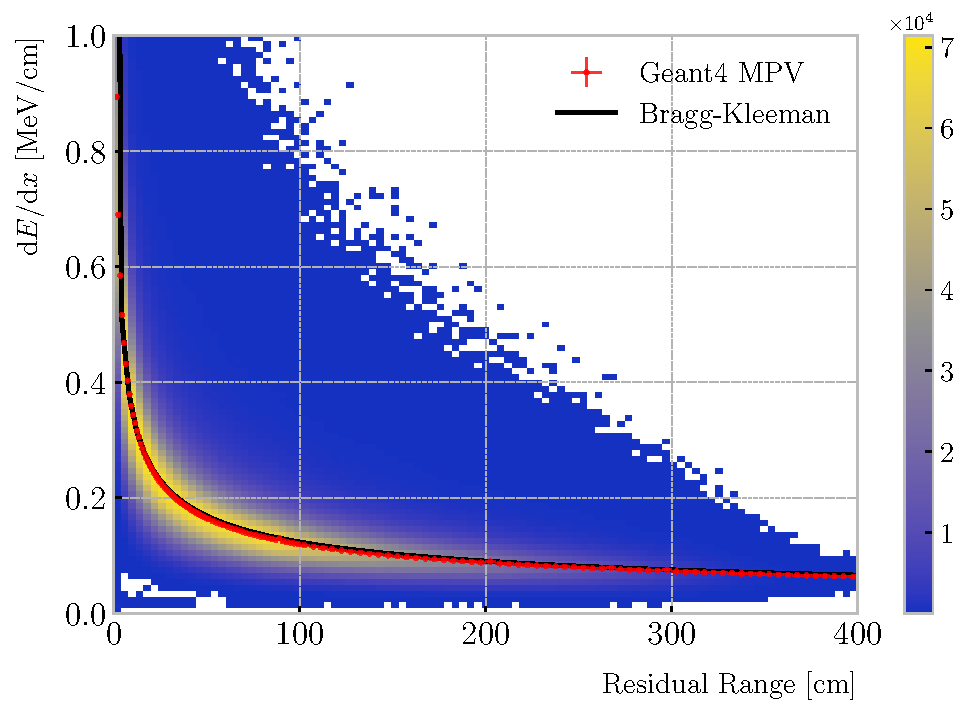
\includegraphics[width=.85\linewidth]{Images/GArSoft_PID/dEdx/bragg_kleeman_geant_langau.pdf}
	\caption[Distribution of the Geant4-simulated energy losses per unit length versus residual range for the stopping proton sample.]{Distribution of the Geant4-simulated energy losses per unit length versus residual range for the stopping proton sample. The overlaid points represent the fitted most probable value of the $\mathrm{d}E/\mathrm{d}x$ distribution in each residual range bin, whereas the curve is their best fit to the Bragg-Kleeman formula from Eq. (\ref{Eq:3.4}).}
	\label{fig:bragg_kleeman}
\end{figure}

At this point, I am left with determining the conversion between the charge deposits per unit length $\mathrm{d}Q/\mathrm{d}x$ and the energy deposits per unit length $\mathrm{d}E/\mathrm{d}x$. To this end, we need a way of comparing the two. I can use the residual range $z$ to get a prediction of the most probable $\mathrm{d}E/\mathrm{d}x$ by using the following empirical parametrisation \cite{Ulmer2010}:
\begin{equation}\label{Eq:3.4}
	\frac{\mathrm{d}E}{\mathrm{d}x}(z) = \frac{z^{\frac{1}{p}-1}}{p\Lambda^{\frac{1}{p}}},
\end{equation}
which is quoted in the literature as the Bragg-Kleeman formula. In order to obtain the $p$ and $\Lambda$ parameters I perform a fit using the energy losses and the residual ranges given by the Geant4 stage of our proton sample.

\begin{figure}[t]
	\centering
	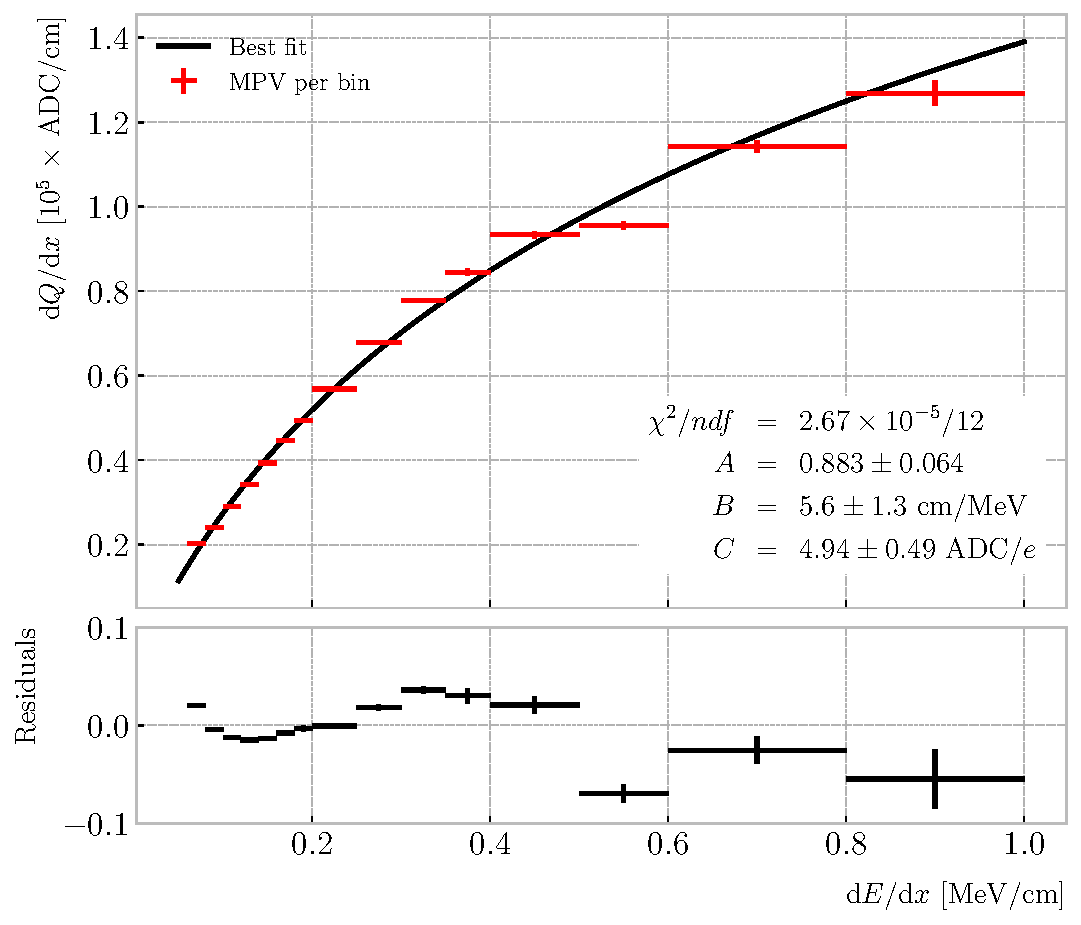
\includegraphics[width=.85\linewidth]{Images/GArSoft_PID/dEdx/dEdx_vs_dQdx_log_fit.pdf}
	\caption[Fitted most probable $\mathrm{d}Q/\mathrm{d}x$ values for each $\mathrm{d}E/\mathrm{d}x$ bin, together with best fit to the logarithmic calibration function.]{Fitted most probable $\mathrm{d}Q/\mathrm{d}x$ values for each $\mathrm{d}E/\mathrm{d}x$ bin (red points), obtained from the stopping proton sample. The overlaid curve (black line) represents the best fit to the logarithmic calibration function from Eq. (\ref{Eq:3.5}).}
	\label{fig:energy_calibration}
\end{figure}

Within our simulation, the residual range is sampled with a maximum size of $5~\mathrm{mm}$. Therefore, to perform the fit to the Bragg-Kleeman formula, we can use a fine-grained residual range binning. For each of the residual range bins I extract the $\mathrm{d}E/\mathrm{d}x$ distribution and fit it to a LanGauss distribution, to obtain the value of the most probable $\mathrm{d}E/\mathrm{d}x$ in the bin together with a statistical uncertainty. I then fit Eq. (\ref{Eq:3.4}) to these most probable values and the centres of the residual range bins. This procedure is depicted in Fig. \ref{fig:bragg_kleeman}, where I show the distribution of the energy loss per unit length versus the residual range, together with the most probable $\mathrm{d}E/\mathrm{d}x$ values and their uncertainty in each bin (red points) and the curve with the best fit of the Bragg-Kleeman relation to those values (black line). The best fit is obtained for the parameter values $p = 1.8192 \pm 0.0005$ and $\Lambda = 0.3497 \pm 0.0008~\mathrm{cm}/\mathrm{MeV}^{p}$\footnote{These strange units for $\Lambda$ come from dimensional analysis, just to keep the Bragg-Kleeman formula (\ref{Eq:3.4}) consistent.}.

Having an analytical expression that relates the residual range to $\mathrm{d}E/\mathrm{d}x$, I can take our reconstruction-level residual ranges from the stopping proton sample and compute the most probable energy loss associated.

In order to parametrise the charge saturation, we can use the following logarithmic function inspired by the modified box model for recombination:
\begin{equation}\label{Eq:3.5}
	\frac{\mathrm{d}E}{\mathrm{d}x} = \frac{\mathrm{e}^{\frac{\mathrm{d}Q}{\mathrm{d}x}B\frac{W_{ion}}{G_{group}C}}-A}{B},
\end{equation}
where $A$ and $B$ are the calibration parameters we need to determine, $W_{ion}$ is the average energy to produce an electron-ion pair, $G_{group}$ is the gain from the reclustering discussed above and $C$ is the calibration constant to convert number of electrons to ADC counts, commonly refer to as gain (also to be obtained in the fit). In this case, I use a value for the electron-ion production energy of $W_{ion} = 26.4 \ \mathrm{eV}$ \cite{Aprile2008}. This value, used in our simulation as well, was measured for gaseous argon in normal conditions, and therefore should be checked in the future to describe correctly the high-pressure argon-$\mathrm{CH}_{4}$ mixture of ND-GAr.

For the calibration fit I follow a procedure similar to the previous one for Eq. (\ref{Eq:3.4}). Binning the $\mathrm{d}E/\mathrm{d}x$ range, I fit a LanGauss distribution to the corresponding $\mathrm{d}Q/\mathrm{d}x$ distribution to obtain the most probable value. The resulting data points (red bars) are shown in Fig. \ref{fig:energy_calibration} (top panel), the horizontal error bars depict the width of the $\mathrm{d}E/\mathrm{d}x$ bin whereas the vertical bars represent the error associated to the most probable value estimation. A fit to the logarithmic function in Eq. (\ref{Eq:3.5}) is also shown (black line). For this I weighted the data points using the inverse of their relative error, obtaining a reduced chi-square value of $\chi^{2}/ndf=2.22\times10^{-6}$. The best fit parameters I found from this fit are $A = 0.883 \pm 0.064$, $B=5.6\pm1.3~\mathrm{cm}/\mathrm{MeV}$ and $C = 4.94 \pm 0.49 \ \mathrm{ADC}/e$. Figure \ref{fig:energy_calibration} (bottom panel) shows the residuals between the data points and the fit.

\begin{comment}
For the calibration fit I follow a procedure similar to the previous one for Eq. (\ref{Eq:3.4}). Binning the $\mathrm{d}E/\mathrm{d}x$ range, I fit a LanGauss distribution to the corresponding $\mathrm{d}Q/\mathrm{d}x$ distribution to obtain the most probable value. The resulting data points (red bars) are shown in Fig. \ref{fig:energy_calibration} (top panel), the horizontal error bars depict the width of the $\mathrm{d}E/\mathrm{d}x$ bin whereas the vertical bars represent the error associated to the most probable value estimation. Two different fits to the logarithmic function in Eq. (\ref{Eq:3.5}) are also shown. In the first case I weighted the data points using the inverse of their relative error (blue line), obtaining a reduced chi-square value of $\chi^{2}/ndf=2.22\times10^{-6}$. The best fit parameters I found from this fit are $A = 0.883 \pm 0.064$, $B=5.6\pm1.3~\mathrm{cm}/\mathrm{MeV}$ and $C = 4.94 \pm 0.49 \ \mathrm{ADC}/e$. In the second case, I performed the fit using unweighted data (yellow line). The reduced chi-square is slightly worse, with $\chi^{2}/ndf=6.95\times10^{-4}$, but the fit parameters fall in a similar range, obtaining $A = 0.76 \pm 0.10$, $B=7.8\pm1.5~\mathrm{cm}/\mathrm{MeV}$ and $C = 5.75 \pm 0.59 \ \mathrm{ADC}/e$. Figure \ref{fig:energy_calibration} (bottom panel) shows the (unweighted) residuals between the data points and the two fits. It can be seen that both fits behave similarly in the low ionisation loss regime, but the unweighted fit manages to capture the behaviour at high energies better.
\end{comment}

\begin{comment}
\begin{table}
	\caption{Calibration parameters obtained from the fit of the ND-GAr simulated stopping proton sample to the calibration function from Eq. (\ref{Eq:3.5}). The fits were performed for the 10, 12, and 16-bit ADC limits and using weighted and unweighted data points, as described in the text.}
	\begin{center}
		\begin{small}
			\begin{tabular}{llllll}
				\cline{3-6}
				\multicolumn{2}{l}{\multirow{2}{*}{}}                                          & \multirow{2}{*}{$\chi^{2}/ndf$} & \multicolumn{3}{l}{Best fit $\pm 1\sigma$}                              \\ \cline{4-6} 
				\multicolumn{2}{l}{}                                                           &                                 & $A$             & $B~(\mathrm{cm}/\mathrm{MeV})$ & $C~(\mathrm{ADC}/e)$ \\ \hline
				\multicolumn{1}{l|}{\multirow{2}{*}{10-bit}} & \multicolumn{1}{l|}{Weighted}   & $1.83\times10^{-6}/12$          & $-9.3\pm3.9$    & $270\pm69$                     & $27.1\pm5.4$         \\
				\multicolumn{1}{l|}{}                        & \multicolumn{1}{l|}{Unweighted} & $2.32\times10^{-3}/12$          & $0.0\pm2.2$     & $86\pm45$                      & $11.4\pm4.5$         \\ \hline
				\multicolumn{1}{l|}{\multirow{2}{*}{12-bit}} & \multicolumn{1}{l|}{Weighted}   & $2.67\times10^{-5}/12$          & $0.883\pm0.064$ & $5.6\pm1.3$                    & $4.94\pm0.49$        \\
				\multicolumn{1}{l|}{}                        & \multicolumn{1}{l|}{Unweighted} & $8.35\times10^{-3}/12$          & $0.76\pm0.10$   & $7.8\pm1.5$                    & $5.75\pm0.59$        \\ \hline
				\multicolumn{1}{l|}{\multirow{2}{*}{16-bit}} & \multicolumn{1}{l|}{Weighted}   & $1.44\times10^{-5}/12$          & $0.949\pm0.024$ & $3.53\pm0.58$                  & $4.52\pm0.29$        \\
				\multicolumn{1}{l|}{}                        & \multicolumn{1}{l|}{Unweighted} & $5.71\times10^{-3}/12$          & $0.850\pm0.054$ & $5.59\pm0.79$                  & $5.43\pm0.39$        \\ \hline
			\end{tabular}
		\end{small}
	\end{center}
	\label{tab:calibration_fits}
\end{table}
\end{comment}

The value for the gain I obtained from the fit is in reasonable agreement with our expectation. This value is set in GArSoft to $5 \ \mathrm{ADC}/e$ by default.

\begin{comment}
\begin{table}[h!]
	\caption{Effective recombination parameters obtained from the fit of ND-GAr simulated stopping proton sample to the modified box model. The corresponding parameters obtained by the LAr TPC experiments ArgoNeuT, $\mu$BooNE and ProtoDUNE are also shown for comparison.}
	\begin{center}
		\begin{tabular}{lcccc}
			\hline
																						   & ArgoNeuT        & $\mu$BooNE     & ProtoDUNE  & ND-GAr \\ \hline
			modified box model $\alpha$                                                    & $0.93\pm0.02$   & $0.92\pm0.02$  & $0.93\pm0.02$ & $0.91\pm0.02$       \\ \hline
			modified box model $\beta'$\\ $(\mathrm{kV/cm})(\mathrm{g/cm^{2}})/\mathrm{MeV}$ & $0.212\pm0.002$ & $0.184\pm0.02$ & $0.20\pm0.03$ & $0.040\pm0.004$     \\ \hline
			\end{tabular}
	\end{center}
	\label{tab:modified_box_fits}
\end{table}
\end{comment}

\begin{figure}[t]
	\centering
	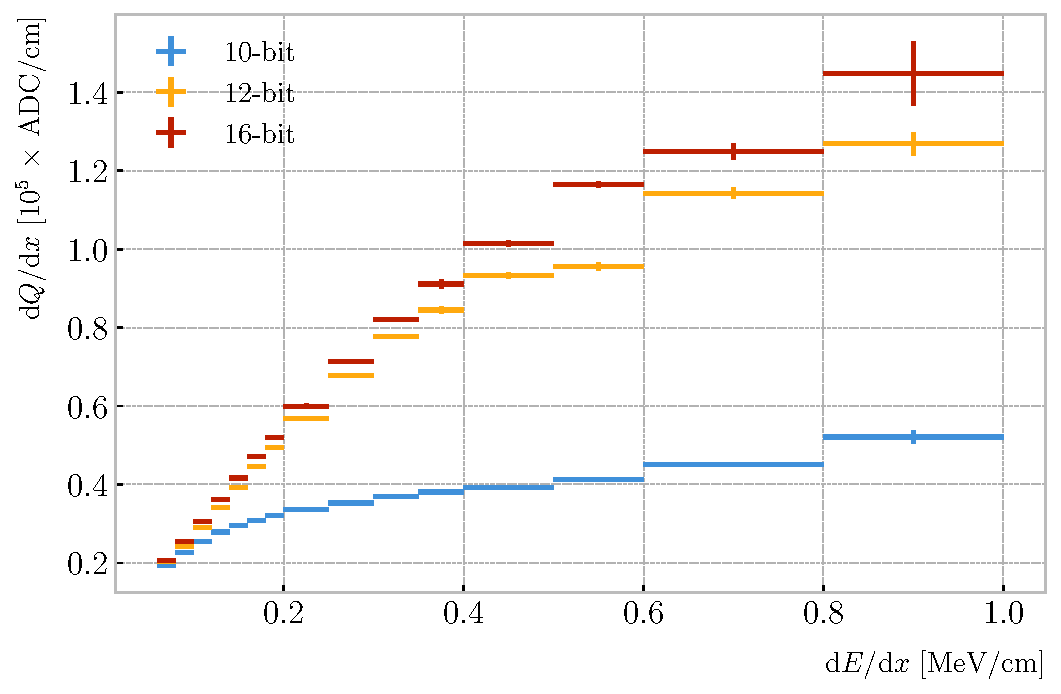
\includegraphics[width=.85\linewidth]{Images/GArSoft_PID/dEdx/dEdx_vs_dQdx_ADC_saturation_mpv.pdf}
	\caption[Fitted most probable $\mathrm{d}Q/\mathrm{d}x$ values for each $\mathrm{d}E/\mathrm{d}x$ bin for three different ADC bit limits.]{Fitted most probable $\mathrm{d}Q/\mathrm{d}x$ values for each $\mathrm{d}E/\mathrm{d}x$ bin for three different ADC bit limits, 10 (blue points), 12 (default, yellow points) and 16-bit (red points).}
	\label{fig:energy_adc_saturation}
\end{figure}

\begin{table}[t]
	\caption[Calibration parameters obtained from the fit of the ND-GAr simulated stopping proton sample to the calibration function, for different ADC limits.]{Calibration parameters obtained from the fit of the ND-GAr simulated stopping proton sample to the calibration function from Eq. (\ref{Eq:3.5}). The fits were performed for the 10, 12, and 16-bit ADC limits.}
	\begin{center}
		\begin{small}
			\begin{tabular}{lllll}
				\cline{2-5}
											& \multirow{2}{*}{$\chi^{2}/ndf$} & \multicolumn{3}{l}{Best fit $\pm 1\sigma$}                              \\ \cline{3-5} 
											&                                 & $A$             & $B~(\mathrm{cm}/\mathrm{MeV})$ & $C~(\mathrm{ADC}/e)$ \\ \hline
				\multicolumn{1}{l|}{10-bit} & $1.83\times10^{-6}/12$          & $-9.3\pm3.9$    & $270\pm69$                     & $27.1\pm5.4$         \\ \hline
				\multicolumn{1}{l|}{12-bit} & $2.67\times10^{-5}/12$          & $0.883\pm0.064$ & $5.6\pm1.3$                    & $4.94\pm0.49$        \\ \hline
				\multicolumn{1}{l|}{16-bit} & $1.44\times10^{-5}/12$          & $0.949\pm0.024$ & $3.53\pm0.58$                  & $4.52\pm0.29$        \\ \hline
			\end{tabular}
		\end{small}
	\end{center}
	\label{tab:calibration_fits}
\end{table}

One interesting thing to check is what induces this non-linear relation between charge and energy. The only effects that modify the amount of electrons reaching the readout planes in the simulation are the transverse diffusion and the finite electron lifetime. Once the electrons reach the readout chambers, the pad response functions are applied, together with an electrons-to-ADC conversion and the ADC saturation limit.

\begin{figure}[t]
	\centering
	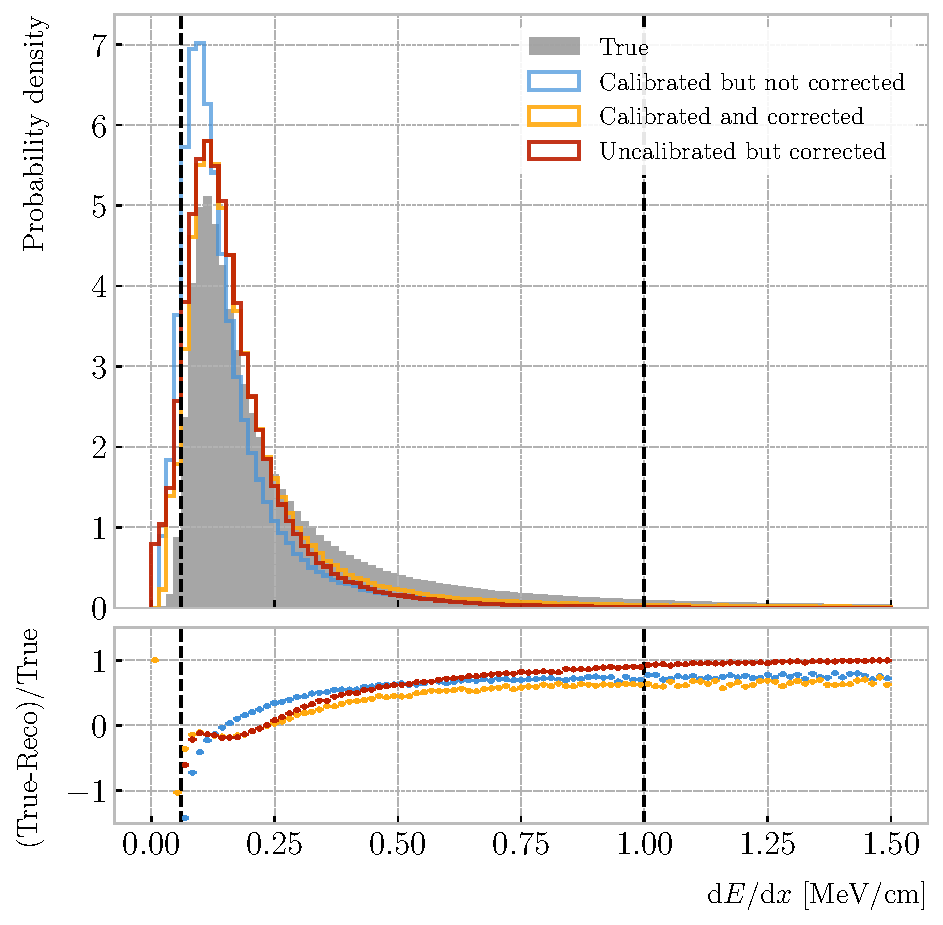
\includegraphics[width=.80\linewidth]{Images/GArSoft_PID/dEdx/reco_dEdx_corrected_1d.pdf}
	\caption[Area normalised $\mathrm{d}E/\mathrm{d}x$ distributions for the true and the reconstructed energy deposits in the stopping proton sample, both after applying the calibration and the calibration and the normalisation correction.]{Top panel: area normalised $\mathrm{d}E/\mathrm{d}x$ distributions for the true (solid grey) and the reconstructed energy deposits in the stopping proton sample, both after applying the calibration (blue) and the calibration and the normalisation correction (yellow). Also shown is the distribution obtained by applying a correction factor to the $\mathrm{d}Q/\mathrm{d}x$ values but not the calibration (red). Bottom panel: fractional residuals for the uncorrected (blue), corrected (yellow) and uncalibrated (red) samples.}
	\label{fig:energy_correction}
\end{figure}

By default, GArSot applies a 12-bit ADC limit, which can be changed in the simulation configuration. However, it can only be increased up to 16-bit, as we represent the ADC collection as a \texttt{std::vector<short>}. This way, I tried to change the saturation parameter to see how it affects the relation between reconstructed charge and energy. Figure \ref{fig:energy_adc_saturation} shows a comparison between the most probable $\mathrm{d}Q/\mathrm{d}x$ for 10, 12 and 16-bit ADC limits. As expected, the lower the limit is the sooner the charge saturates. For higher ADC limits the relation between energy and charge remains linear up to higher $\mathrm{d}E/\mathrm{d}x$ values, but even for the 16-bit limit the saturation is noticeable for values $\gtrsim 0.5 ~ \mathrm{MeV}/\mathrm{cm}$.

Table \ref{tab:calibration_fits} shows the results of fitting the samples with 10 and 16-bits ADC limits to the calibration function from Eq. (\ref{Eq:3.5}), using the weights based on their relative error as described previously. One interesting feature to notice is how different the best fit points look for the 10-bit ADC saturation when compared to the other two, which are consistent with each other.

At this point we can compare the $\mathrm{d}E/\mathrm{d}x$ distribution one gets from Geant4, i.e. the true energy loss distribution, and the distribution I found by applying the calibration function to our collection of reconstructed $\mathrm{d}Q/\mathrm{d}x$ values. Figure \ref{fig:energy_correction} (top panel) shows the true (solid grey) and reconstructed (blue, labeled as uncorrected) distributions together. The dashed vertical lines indicate the region of validity of the calibration fit, i.e. the left and right edges of the first and last $\mathrm{d}E/\mathrm{d}x$ bin respectively. Notice that these histograms are area-normalised, as the total number of true energy deposits is much higher than the number of reconstructed charge deposits. This is due to a combination of effects, like the finite spatial resolution of the detector, the hit clustering used in the track fitting and the reclustering we have applied here.

The two distributions are significantly different. That can be seen clearly when looking at the fractional residuals, shown in Fig. \ref{fig:energy_correction} (bottom panel). In particular, the position of the peak is off, which could bias the mean energy loss predictions. It seems like the difference between these may be due to an overall scaling factor. One possibility is to scale the most probable value of the reconstructed distribution to the most probable value predicted by Geant4. I do this by fitting both distributions using a LanGauss function, obtaining $\mathrm{d}E/\mathrm{d}x_{\mathrm{MPV}, ~true} = 0.1145\pm0.0005~\mathrm{MeV}/\mathrm{cm}$ and $\mathrm{d}E/\mathrm{d}x_{\mathrm{MPV}, ~reco} = 0.0928\pm0.0005~\mathrm{MeV}/\mathrm{cm}$ for the true and reconstructed most probable values respectively. These can be translated into an scaling factor $S=0.579\pm0.006$.

The result of applying the scaling correction can be seen in Fig. \ref{fig:energy_correction} (top panel). The corrected $\mathrm{d}E/\mathrm{d}x$ distribution (yellow, labeled as corrected) peaks around the same value the true distribution does, as expected. Moreover, the high energy region is also slightly better described. For low ionisations, below the lower limit of the calibration fit, the differences between true and reconstructed are still significant. This low energy excess may be migration of some events from the peak region. The overall effect of the correction can be seen in the fractional residual plot in Fig. \ref{fig:energy_correction} (bottom panel).

One can also check what happens if instead of applying the logarithmic calibration we simply scale the $\mathrm{d}Q/\mathrm{d}x$ distribution (post reclustering) to have the same most probable value as the true  $\mathrm{d}E/\mathrm{d}x$ distribution. In this case, following an analogous procedure to the one described earlier, I found the scaling factor $S_{uncalibrated}=0.414\pm0.002~\mathrm{MeV}/\mathrm{ADC}$\footnote{Notice that now the scaling factor is not dimensionless, as it acts more like a conversion factor here.}. The resulting distribution (red, labeled as uncalibrated) is also shown in in Fig. \ref{fig:energy_correction} (top panel). The behaviour of the new distribution is similar to the corrected case at low energy losses, around the peak of the true distribution, but it is worse at describing the high energy tail. This is expected, it is in the high ionisation regime where saturation effects apply and therefore calibration is needed.

\subsection[Truncated \texorpdfstring{$\mathrm{d}E/\mathrm{d}x$}{dE/dx} mean]{Truncated \boldmath\texorpdfstring{$\mathrm{d}E/\mathrm{d}x$}{dE/dx} mean} \label{subsec:mean_dEdx}

\begin{figure}[t]
	\centering
	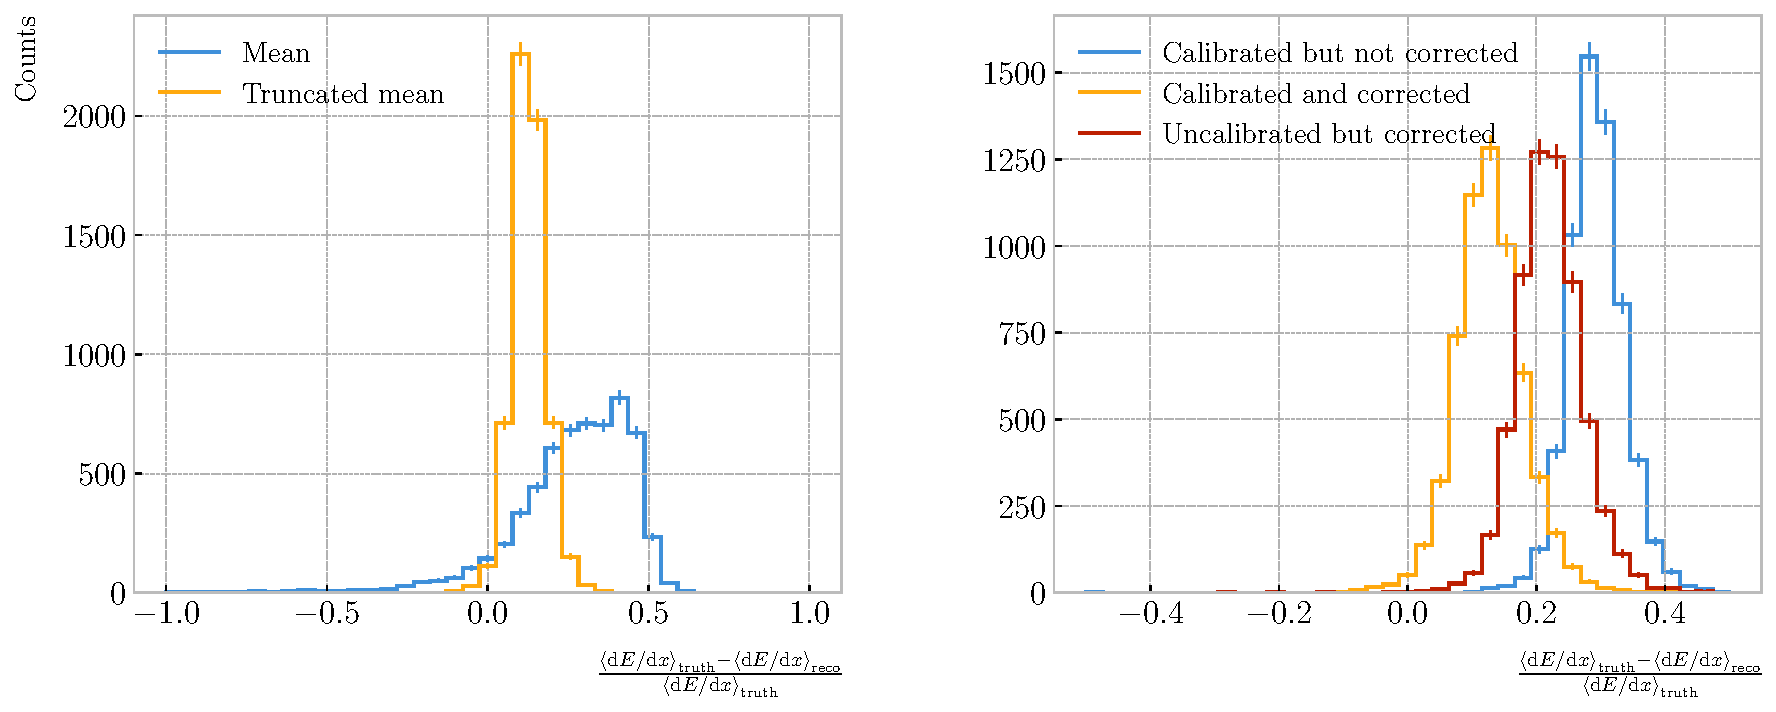
\includegraphics[width=.90\linewidth]{Images/GArSoft_PID/dEdx/reco_dEdx_truncation_comp.pdf}
	\caption[Fractional residuals between the true and the corrected $\mathrm{d}E/\mathrm{d}x$ means and the $60\%$ truncated means, and fractional residuals between the true and the uncorrected, corrected and uncalibrated $\mathrm{d}E/\mathrm{d}x$ $60\%$ truncated means.]{Left panel: fractional residuals between the true and the corrected $\mathrm{d}E/\mathrm{d}x$ means (blue) and the $60\%$ truncated means (yellow), for each event in the stopping proton sample. Right panel: fractional residuals between the true and the uncorrected (blue), corrected (yellow) and uncalibrated (red) $\mathrm{d}E/\mathrm{d}x$ $60\%$ truncated means, for each event in the stopping proton sample.}
	\label{fig:energy_trucation_comp}
\end{figure}

Once we have a collection of $\mathrm{d}E/\mathrm{d}x$ values for each reconstructed track, we can compute the corresponding most probable ionisation loss per unit length of the particle. This is the value predicted by the Bethe-Bloch or the PAI models, and together with a measurement of the momentum it allows for particle identification.

However, estimating the most probable $\mathrm{d}E/\mathrm{d}x$ value for each reconstructed track is not a trivial task. As mentioned before, the $\mathrm{d}E/\mathrm{d}x$ distributions follow Landau-like distributions. Therefore, one should perform e.g. a LanGauss fit to correctly estimate the most probable values. Automating this kind of fits is often problematic, as they usually incur in convergence problems. Moreover, the reconstructed $\mathrm{d}E/\mathrm{d}x$ distributions we obtain tend to have relatively small statistics, which may also produce poor fits. In practice, doing these unsupervised fits may degrade our performance, and a more robust method is preferred.

A possibility could be taking the mean of the reconstructed $\mathrm{d}E/\mathrm{d}x$ distribution for each particle. The problem with this approach is that the high energy Landau tail, combined with our limited statistics, can induce large fluctuations in the computation of the mean. Imagine you have two protons with the same kinetic energy, but due to reconstruction problems in one case you did not get as many charge deposits reconstructed in its high ionisation loss region. If you do not remove the tails the computed $\mathrm{d}E/\mathrm{d}x$ means will be significantly different.

\begin{figure}[t]
	\centering
	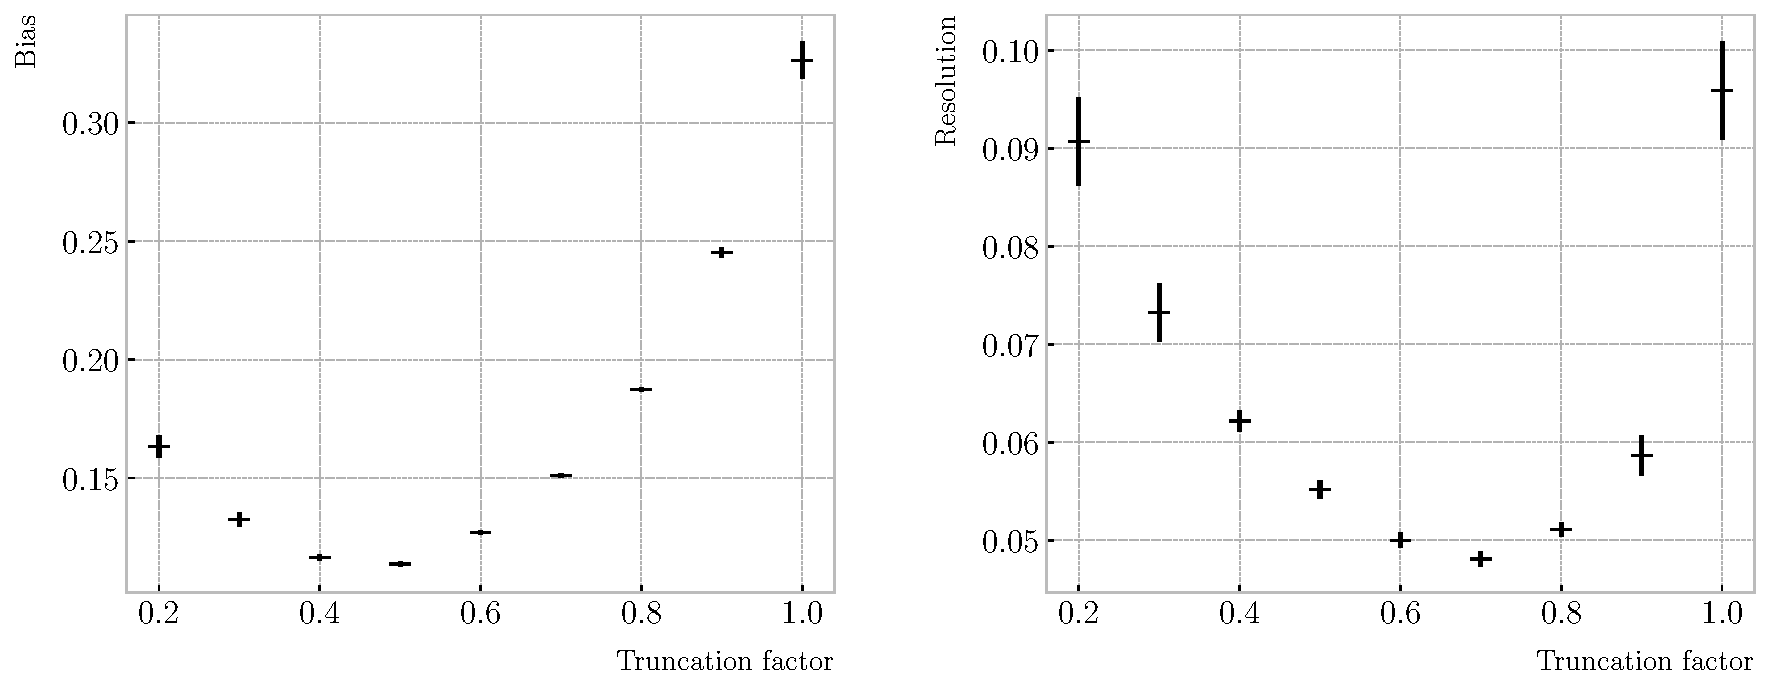
\includegraphics[width=.90\linewidth]{Images/GArSoft_PID/dEdx/reco_dEdx_truncation_opt.pdf}
	\caption[Estimated values of the mean $\mathrm{d}E/\mathrm{d}x$ bias and resolution for the stopping proton sample at different values of the truncation factor.]{Estimated values of the mean $\mathrm{d}E/\mathrm{d}x$ bias (left panel) and resolution (right panel) obtained using the corrected data from the stopping proton sample, for different values of the truncation factor.}
	\label{fig:energy_trucation_opt}
\end{figure}

In order to avoid those fluctuations, one can compute the mean of a truncated $\mathrm{d}E/\mathrm{d}x$ distribution instead. By keeping only a given fraction of the lowest energy deposits we obtain an estimate of the mean energy loss that is more resilient to reconstruction inefficiencies and statistical effects. Figure \ref{fig:energy_trucation_comp} (left panel) shows a comparison between the $\left<\mathrm{d}E/\mathrm{d}x\right>$ computed by taking the mean of the full distribution (blue line) and the $60\%$ lowest energy clusters (yellow line), for the stopping proton sample. The fractional residuals are computed for each proton, taking the corresponding means using their collections of true and reconstructed energy deposits. One can see that using the simple mean translates into a high bias and uncertainty in the $\left<\mathrm{d}E/\mathrm{d}x\right>$ estimation, whereas applying the truncation reduces both significantly.

Additionally, I performed a comparison between the $60\%$ truncated mean $\mathrm{d}E/\mathrm{d}x$ obtained using the different calibration methods discussed earlier, namely the uncorrected (blue), corrected (yellow) and uncalibrated (red) distributions. The results are shown in Fig. \ref{fig:energy_trucation_comp} (right panel). While the widths of these distributions are similar, the bias obtained for the corrected sample, i.e. calibration function and correction factor applied, is a factor of $\sim2$ lower than in the uncalibrated case and almost three times smaller than for the uncorrected sample.

The next step is to optimise the level of truncation we are going to apply to our data. To do so, I used different truncation factors, i.e. the percentage of energy-ordered reconstructed energy deposits we keep to compute the mean, on the corrected $\mathrm{d}E/\mathrm{d}x$ sample of the stopping protons. Then, following the same procedure of computing the fractional residuals as before, I fitted the resulting histograms using a double Gaussian function. This is simply the sum of two Gaussian functions of the type:
\begin{equation}
	g(x;~\mu, \sigma, A) = A~\mathrm{e}^{-\frac{(x-\mu)^{2}}{2\sigma^{2}}}.
\end{equation}
I do not add the classical normalisation factor of the Gaussian, $1/\sqrt{2\pi}\sigma$, therefore the amplitude $A$ simply represents the maximum of the function. One of the two Gaussian functions describes the core part of the distribution, while the other captures the behaviour of the tails.

For each truncation factor, I look at the bias and the resolution I obtain. I define these as the weighted means of the corresponding parameters in the fits:
\begin{equation}
	\bar{x} = \frac{A_{core}~x_{core}+A_{tail}~x_{tail}}{A_{core}+A_{tail}},
\end{equation}
where $A_{core}$ and $A_{tail}$ are the amplitudes of the core and tail distributions respectively and $x$ is either the mean $\mu$ or the width $\sigma$ of said distributions.

Figure \ref{fig:energy_trucation_opt} shows the bias (left panel) and the resolution (right panel) I obtained for the stopping proton sample, using different values of the truncation. From these, it can be seen that a truncation factor of $50\%$ minimises the bias in the estimation, while $70\%$ gives the best resolution. That way, I settled on the intermediate value of $60\%$ truncation, which yields a $\left<\mathrm{d}E/\mathrm{d}x\right>$ resolution of $5.00\pm0.08~\%$ for stopping protons.

\subsection[Mean \texorpdfstring{$\mathrm{d}E/\mathrm{d}x$}{dE/dx} parametrisation]{Mean \boldmath\texorpdfstring{$\mathrm{d}E/\mathrm{d}x$}{dE/dx} parametrisation}

\begin{figure}[t]
	\centering
	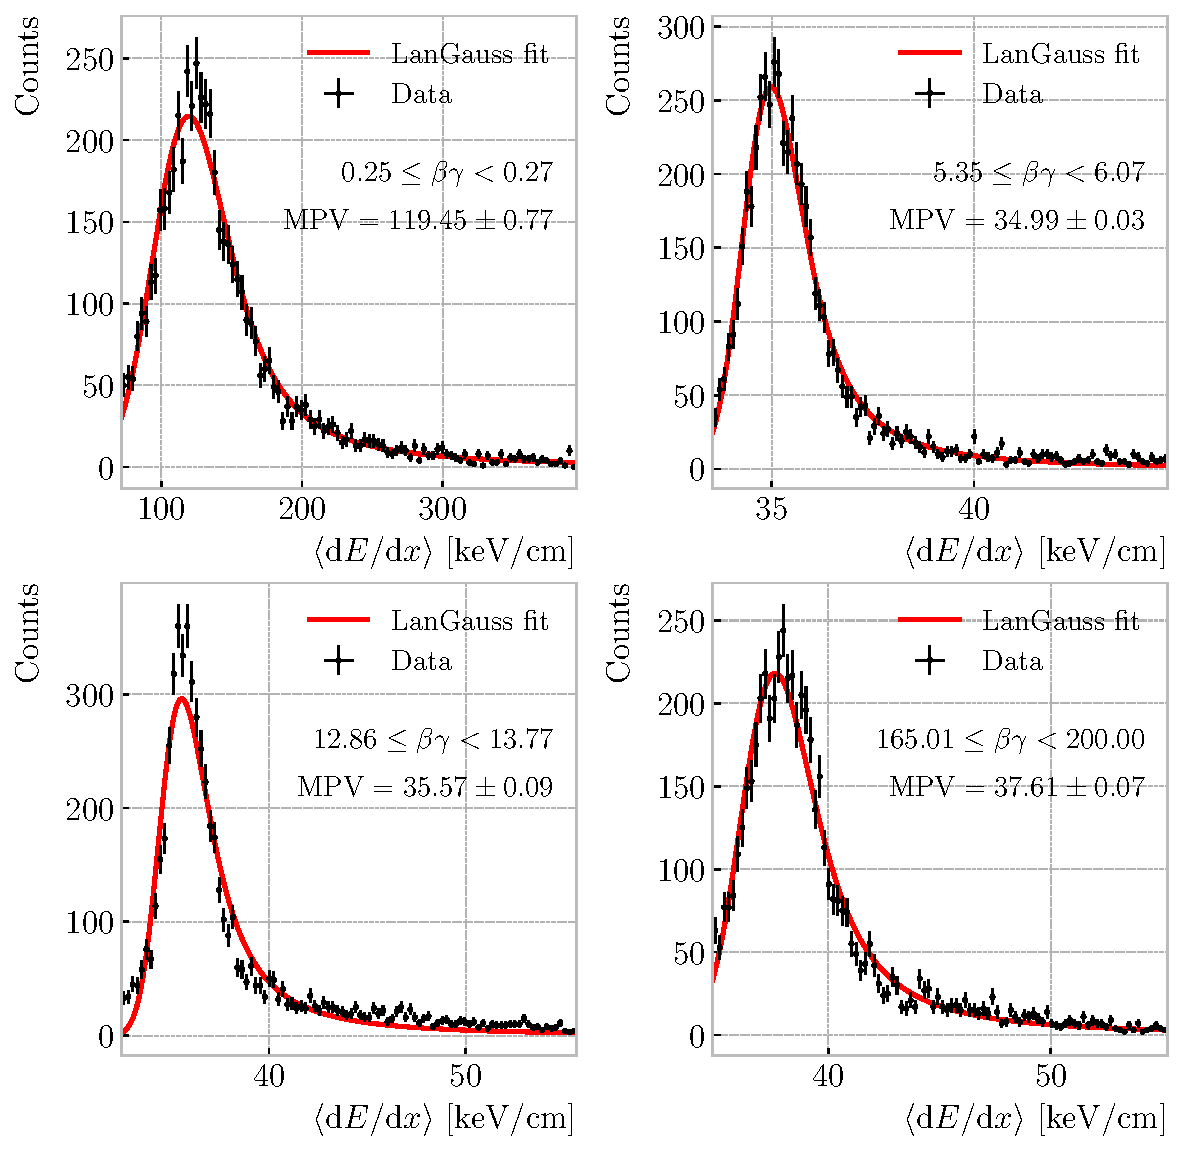
\includegraphics[width=.85\linewidth]{Images/GArSoft_PID/dEdx/dEdx_betagamma_examples.pdf}
	\caption[Examples of the truncated mean $\mathrm{d}E/\mathrm{d}x$ LanGauss fits for various $\beta\gamma$ bins, from a simulated FHC neutrino sample.]{Examples of the truncated mean $\mathrm{d}E/\mathrm{d}x$ LanGauss fits for various $\beta\gamma$ bins, from a simulated FHC neutrino sample.}
	\label{fig:dEdx_betagamma_fits}
\end{figure}

Now that we have a way to estimate the mean energy loss of a particle in the HPgTPC, we can determine the value of the free parameters in the \gls{aleph} formula, Eq. (\ref{Eq:3.3}). For this, I used a sample of $10^{5}$ reconstructed FHC neutrino events inside ND-GAr. In this case I cannot use the stopping proton sample, as we need to cover the full kinematic range of interest for the neutrino interactions in our detector.

The original data does not contain an estimation of the velocity of the tracks, instead the tracks have a value for the reconstructed momentum and the associated PDG code of the Geant4-level particle that created the track. Therefore, one can select some of the particles in the data, in this case I selected electrons, muons, pions and protons, and compute $\beta$ and $\gamma$ using the reconstructed momentum and their mass. In terms of $\beta\gamma$ the mean $\mathrm{d}E/\mathrm{d}x$ does not depend on the particle species, so one can consider all the dataset as a whole. For this fit, I will express $\beta$ in terms of the $\beta\gamma$ product as:
\begin{equation}
    \beta = \frac{\beta\gamma}{\sqrt{1+(\beta\gamma)^{2}}},
\end{equation}
which can be easily proven from the definition of $\gamma$.

\begin{figure}[t]
	\centering
	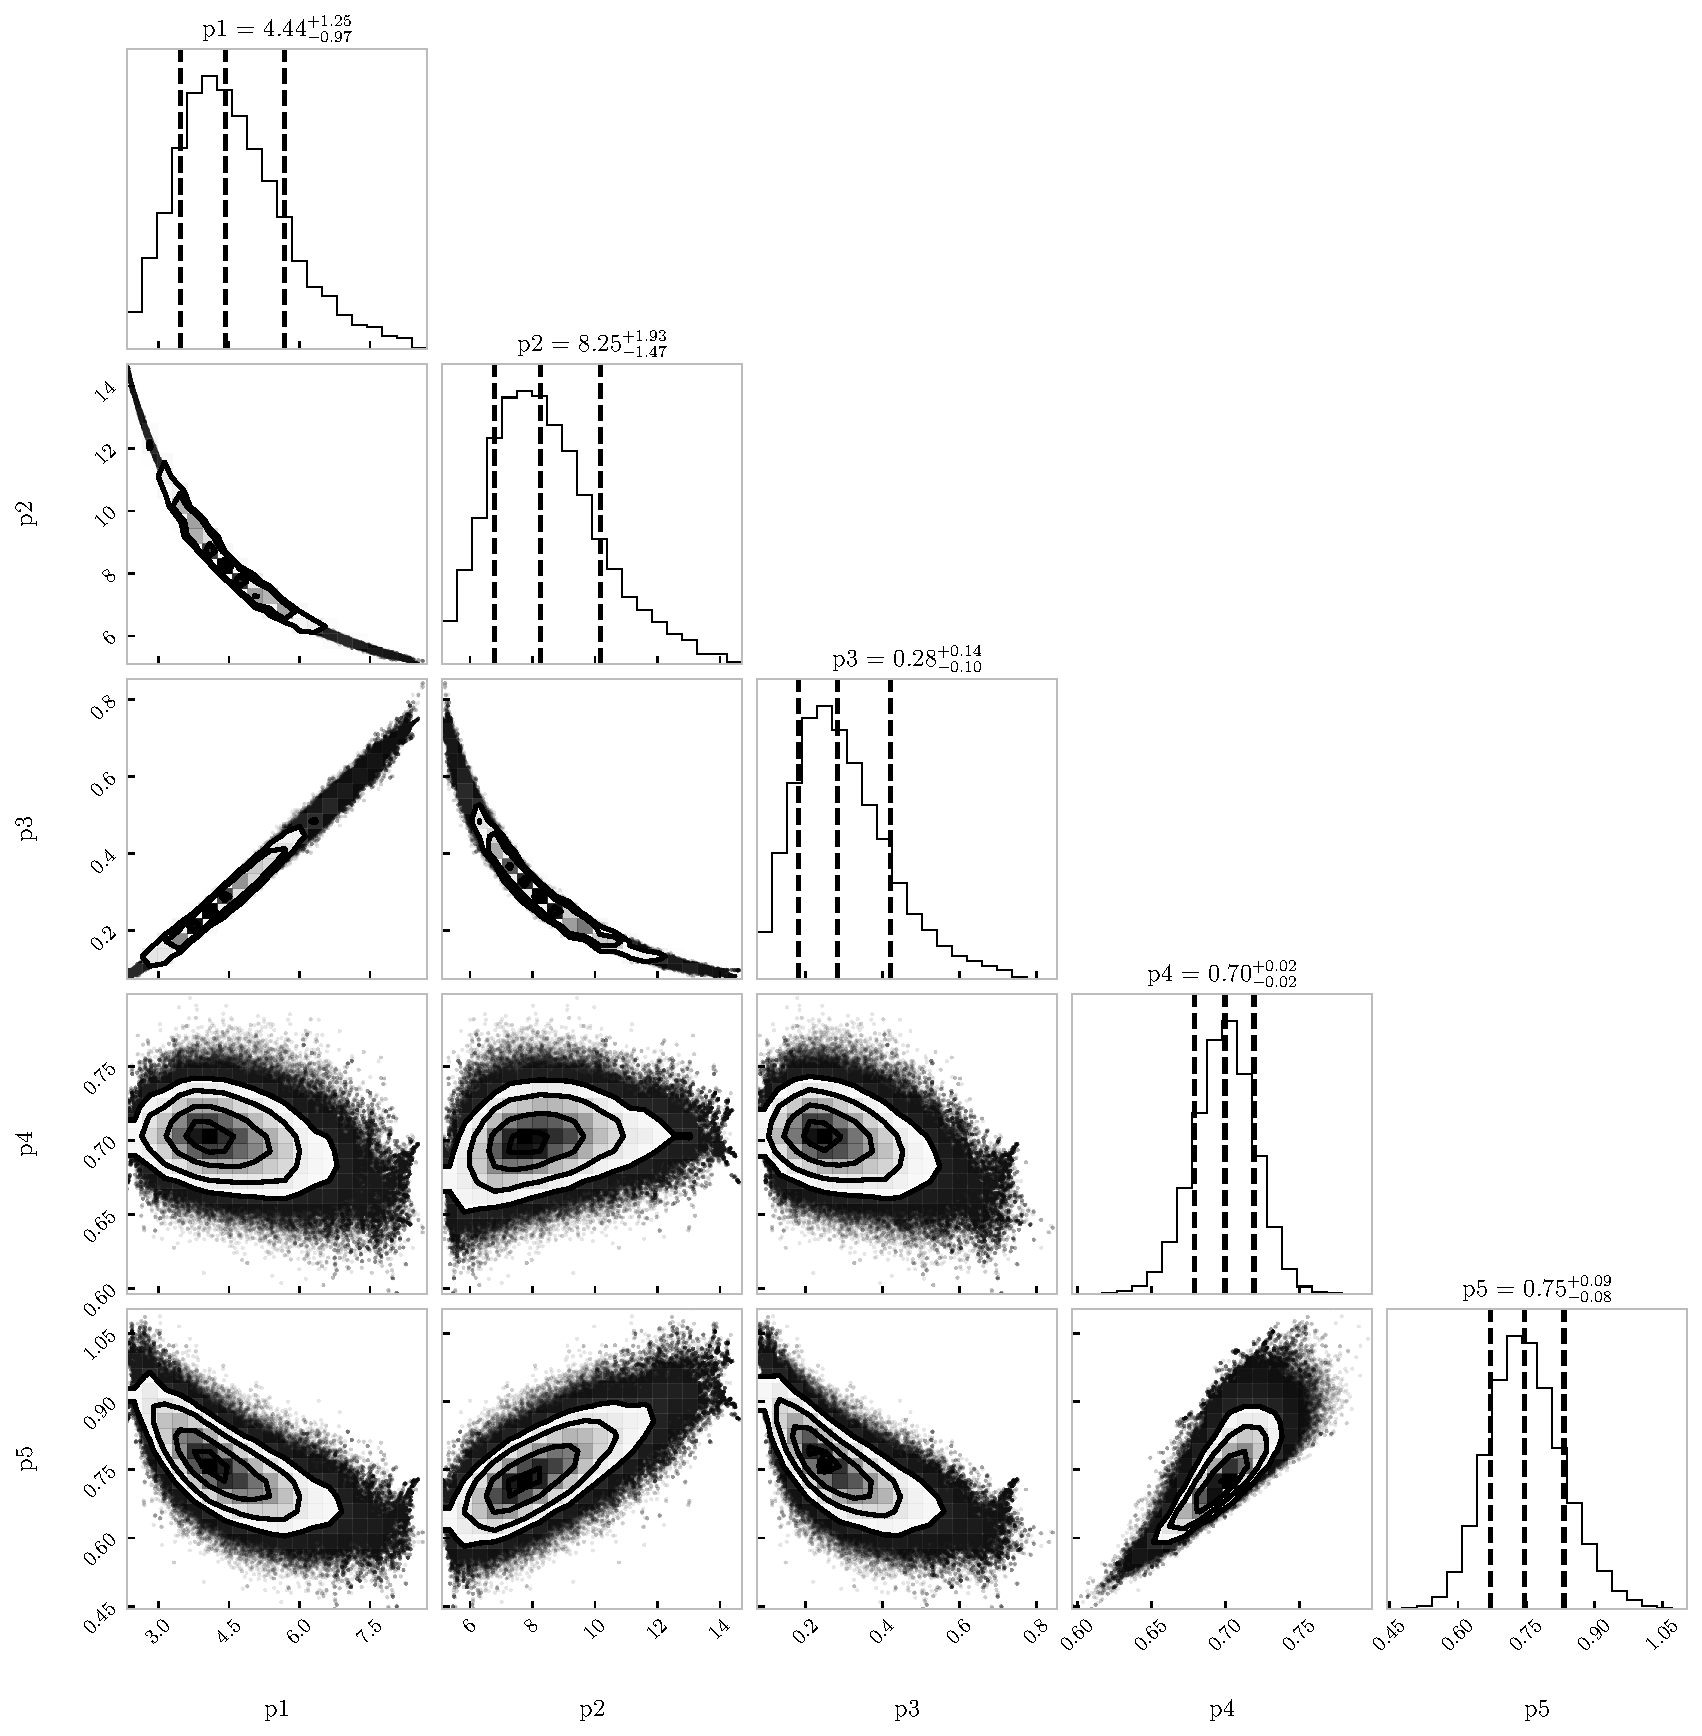
\includegraphics[width=.85\linewidth]{Images/GArSoft_PID/dEdx/mcmc_weighted_equal_frequency_bin_200.pdf}
	\caption[Resulting one and two dimensional projections of the posterior probability distributions of the \gls{aleph} $\left<\mathrm{d}E/\mathrm{d}x\right>$ parameters obtained by fitting the $60\%$ truncated mean $\mathrm{d}E/\mathrm{d}x$ values from a FHC neutrino sample.]{Resulting one and two dimensional projections of the posterior probability distributions of the \gls{aleph} $\left<\mathrm{d}E/\mathrm{d}x\right>$ parameters obtained by fitting the $60\%$ truncated mean $\mathrm{d}E/\mathrm{d}x$ values from a FHC neutrino sample in ND-GAr. The vertical dashed lines in the 1D distributions represent the 16th, 50th and 84th percentiles.}
	\label{fig:dEdx_aleph_fit}
\end{figure}

Next, I bin the data in $\beta\gamma$. I chose a fine binning so as to capture the different features of the ionisation curve. Instead of fixing the bin width, I select them so each one has approximately the same statistics. Then, for each $\beta\gamma$ slice, I compute the median and the interquartile range (IQR) of the $\left<\mathrm{d}E/\mathrm{d}x\right>$ distribution. Using these, I make a histogram in the range $[\mathrm{median}-\mathrm{IQR},~ \mathrm{median}+5~\mathrm{IQR})$, which I fit to a LanGauss function in order to extract the MPV. Using this range accounts for the asymmetric nature of the distributions, while also helps avoiding a second, lower maximum present at low $\beta\gamma$, probably a result of reconstruction failures.

\begin{figure}[t]
	\centering
	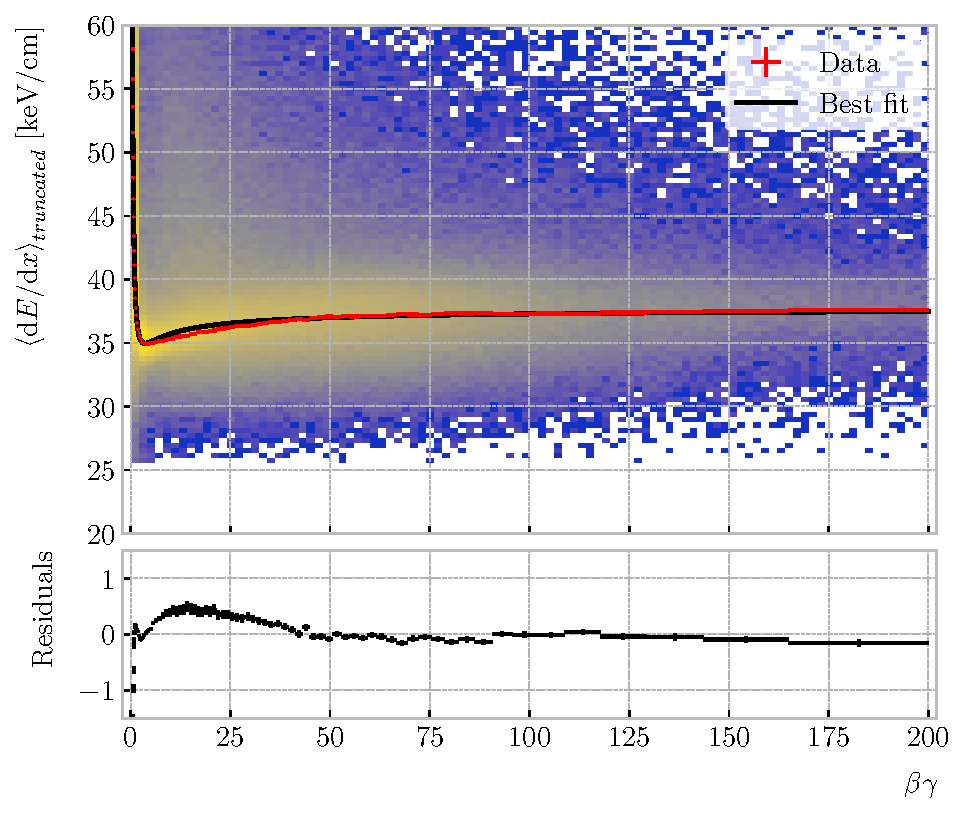
\includegraphics[width=.85\linewidth]{Images/GArSoft_PID/dEdx/dEdx_aleph_data_with_fit.pdf}
	\caption[Truncated mean $\mathrm{d}E/\mathrm{d}x$ obtained for the FHC neutrino sample as a function of the $\beta\gamma$ product, together with the fitted most probable values for each $\beta\gamma$ bin and the best fit obtained using the \gls{aleph} parametrisation.]{Truncated mean $\mathrm{d}E/\mathrm{d}x$ obtained for the FHC neutrino sample as a function of the $\beta\gamma$ product (upper panel). Also shown are the fitted most probable values for each $\beta\gamma$ bin (red points) and the best fit obtained using the \gls{aleph} parametrisation (black line). The residuals resulting from the fit are shown in the lower panel.}
	\label{fig:dEdx_betagamma_aleph}
\end{figure}

A few examples of these fits are shown in Fig. \ref{fig:dEdx_betagamma_fits}. The chosen values of $\beta\gamma$ sit in very distinct points along the $\left<\mathrm{d}E/\mathrm{d}x\right>$ curve, going from the high ionisation region at low velocities (top left panel), to the minimum point (top right panel), the beginning of the relativistic rise (bottom left panel), and the plateau produced by the density effect (bottom right panel).

I used the resulting most probable $\left<\mathrm{d}E/\mathrm{d}x\right>$ values and the centres of the $\beta\gamma$ bins as the points to fit to the \gls{aleph} formula. For this particular fit I used the least-squares method to get a first estimation of the \gls{aleph} parameters. Applying some uniform priors, I then used these values as the starting point of a $100000$ steps MCMC. Figure \ref{fig:dEdx_aleph_fit} shows the posterior probability distributions I obtain for each parameter. The reported best fit points are based on the 16th, 50th, and 84th percentiles in the marginalised distributions.

\begin{figure}[t]
	\centering
	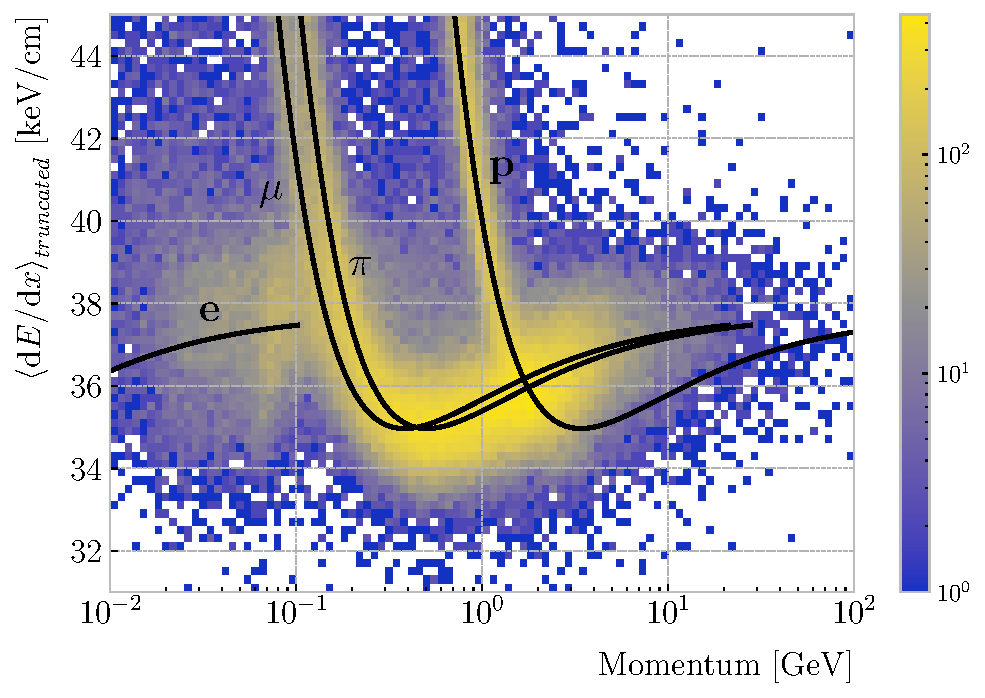
\includegraphics[width=.90\linewidth]{Images/GArSoft_PID/dEdx/dEdx_curves_with_fit.pdf}
	\caption[Distribution of the $60\%$ truncated mean $\mathrm{d}E/\mathrm{d}x$ versus reconstructed momentum for the FHC neutrino sample.]{Distribution of the $60\%$ truncated mean $\mathrm{d}E/\mathrm{d}x$ versus reconstructed momentum for the FHC neutrino sample. The black lines indicate the predictions of the \gls{aleph} parametrisation for electrons, muons, charged pions and protons.}
	\label{fig:dEdx_vs_momentum}
\end{figure}

The resulting fit (black line), compared to the data points (red points) and the underlying distribution is shown in Fig. \ref{fig:dEdx_betagamma_aleph} (top panel). The overall fit is good, with a reduced chi-squared of $\chi^{2}/ndf=1.02$. However, there are some regions where the fit does not describe the data correctly, like the very low $\beta\gamma$ regime, where the fit severely underestimates for energy losses $\gtrsim 50 ~ \mathrm{keV}/\mathrm{cm}$, and the start of the relativistic raise, where we have a slight overestimation. This is a result of those points having a larger uncertainty when compared to the ones around the dip or the plateau areas. These differences can be better seen in the residual plot, Fig. \ref{fig:dEdx_betagamma_aleph} (bottom panel).

\begin{comment}
\begin{table}[t]
	\caption{Best fit parameters obtained fitting a ND-GAr simulated FHC neutrino sample to the \gls{aleph} mean $\mathrm{d}E/\mathrm{d}x$ parametrisation from Eq. (\ref{Eq:3.3}).}
	\begin{center}
		\begin{small}
			\begin{tabular}{l|l|l}
				Parameter & Best fit $\pm 1\sigma$ & $3\sigma$ range \\ \hline
				$P_{1}$   &                        &                 \\
				$P_{2}$   &                        &                 \\
				$P_{3}$   &                        &                 \\
				$P_{4}$   &                        &                 \\
				$P_{5}$   &                        &                
			\end{tabular}
		\end{small}
	\end{center}
	\label{tab:aleph_fit}
\end{table}
\end{comment}

\subsection{Particle identification}

\begin{figure}[t]
	\centering
	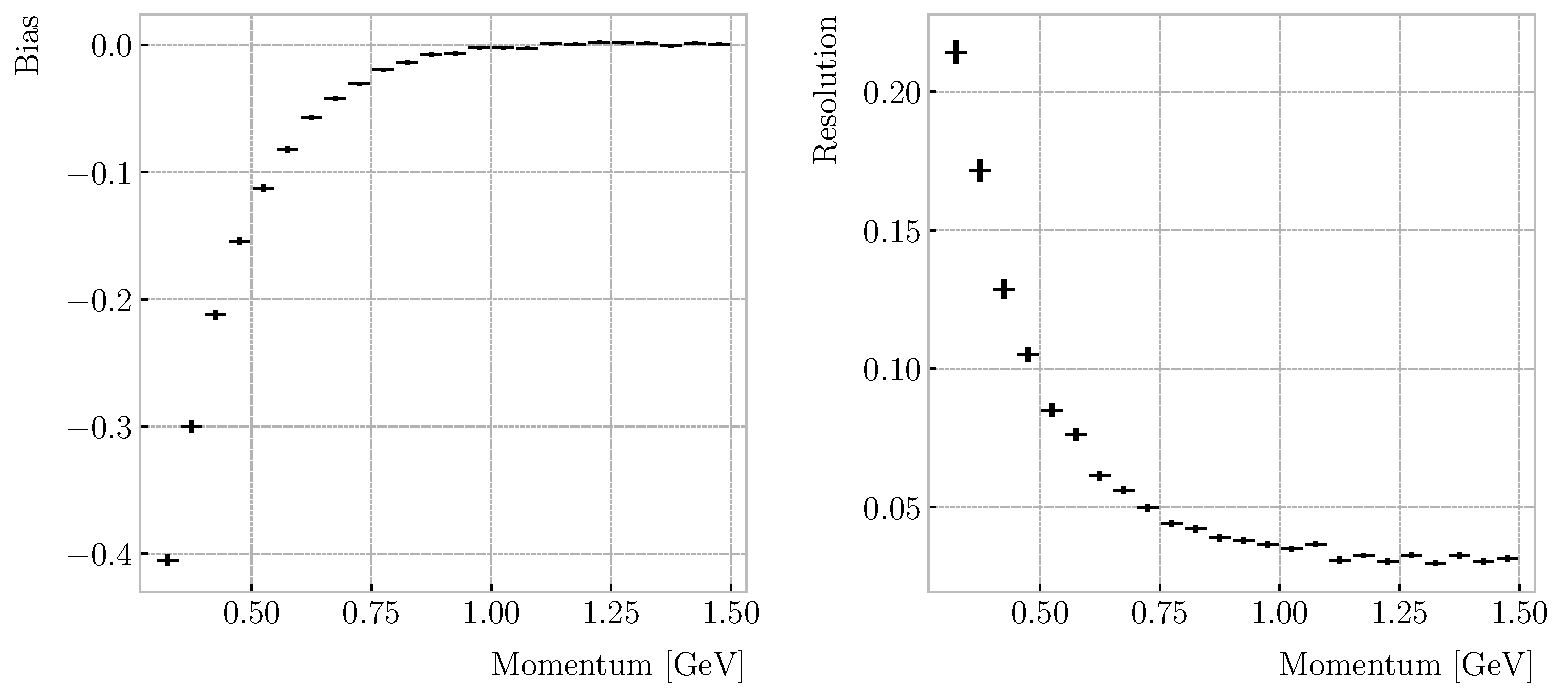
\includegraphics[width=.90\linewidth]{Images/GArSoft_PID/dEdx/proton_dEdx_momentum.pdf}
	\caption[Estimated values of the mean $\mathrm{d}E/\mathrm{d}x$ bias and resolution obtained for the true protons in a FHC neutrino sample.]{Estimated values of the mean $\mathrm{d}E/\mathrm{d}x$ bias (left panel) and resolution (right panel) obtained for the true protons in a FHC neutrino sample.}
	\label{fig:proton_dEdx_momentum}
\end{figure}

\section{Muon and pion separation in the ECal and MuID}\label{section:muon_bdt}

\begin{figure}[t]
	\centering
	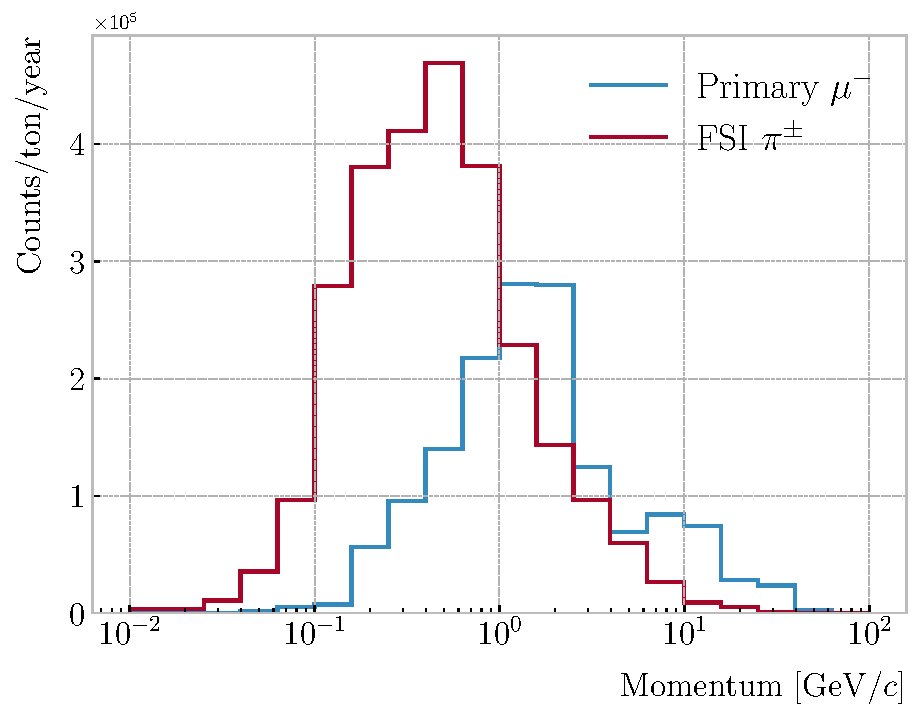
\includegraphics[width=.70\linewidth]{Images/GArSoft_PID/BDT/ndgar_fhc_numu_cc_mu_spectrum.pdf}
	\caption[True momentum distribution for the primary muon in $\nu_{\mu}$ CC $N\pi^{\pm}$ interactions inside the fiducial volume of ND-GAr, compared to the post FSI charged pion spectrum.]{True momentum distribution for the primary muon in $\nu_{\mu}$ CC $N\pi^{\pm}$ interactions inside the fiducial volume of ND-GAr (blue line), compared to the post FSI charged pion spectrum (red line).}
	\label{fig:primary_muon_spectrum}
\end{figure}

As it could be seen from Fig. \ref{fig:dEdx_vs_momentum}, it is not possible to separate muons and charged pions in the HPgTPC using $\mathrm{d}E/\mathrm{d}x$ for momenta $\gtrsim 300~\mathrm{MeV}/c$. In ND-GAr, approximately $70\%$ of the interactions in FHC mode will be $\nu_{\mu}$ CC (compared to the $47\%$ of $\bar{\nu}_{\mu}$ CC interactions when operating in RHC mode), while $24\%$ are neutral currents. Out of these, around $53\%$ and $47\%$ of them will produce at leat one charged pion in the final state, respectively. Figure \ref{fig:primary_muon_spectrum} shows a comparison between the spectra of the primary muons and the charged pions for $\nu_{\mu}$ CC interactions in ND-GAr producing one or more charged pions. From this, one can see that (i) the majority of muons and charged pions are not going to be distinguishable with a $\left<\mathrm{d}E/\mathrm{d}x\right>$ measurement, and that (ii) particle identification in necessary both to classify correctly the $\nu_{\mu}$ CC events and identify the primary muon within them.

ND-GAr features two other subdetectors which can provide additional information for this task, namely the ECal and MuID. The current ECal design, described in (ref section), consists of $42$ layers, made of $5~\mathrm{mm}$ of Pb, $7~\mathrm{mm}$ of plastic scintillator and a $1~\mathrm{mm}$ PCB board. The total thickness of this calorimeter is $1.66$ nuclear interaction lengths or $1.39$ pion interaction lengths. The MuID design is in a more conceptual stage, however it is envisioned to feature layers with $10~\mathrm{cm}$ of Fe and $2~\mathrm{cm}$ of plastic scintillator\footnote{It is not mentioned anywhere, but I assume that there should also be another layer of PCB board of $1~\mathrm{mm}$. However, in this case its contribution to the total thickness of the sampling calorimeter would be negligible.}. With its three layers, it will have a thickness of $1.87$ or $1.53$ nuclear or pion interaction lengths, respectively.

Because pion showers are dominated by inelastic nuclear interactions, the signatures of these particles in the calorimeter will look significantly different from those of muons. Although our ECal is not thick enough to fully contain the hadronic showers of the charged pions at their typical energies in FHC neutrino interactions, they can still be used to understand whether the original particle was more hadron-like or MIP-like. In Fig. \ref{fig:ecal_example} I show two examples of energy distributions created by a muon (left panel) and a charged pion (right panel) of similar momenta interacting in the ECal. These figures represent the transverse development of the interactions. For each of them, I computed the principal component and centre of mass of the interaction, projecting the position of the hits onto the plane perpendicular to that direction, and taking the distances relative to the centre. It can be seen that the muon follows an almost MIP-like behaviour, being the central bin in the histogram the one with the highest deposited energy. On the other hand, the pion not only deposits more energy overall, but also this energy is more spread-out among the different hits. It is this kind of information that would allow us to tell apart muons from pions.

This way, I identify three main action points that need to be addressed if one wants to use these detectors to distinguish between muons and charged pions. These are:
\begin{enumerate}
	\item the way we make the associations between tracks in the HPgTPC to the activities (what in GArSoft we call clusters) in the ECal and the MuID,
	\item what variables or features one can extract from the calorimeters that encapsulate the information we are interested about,
	\item and how to carry out the classification problem.
\end{enumerate}

\begin{figure}[t]
	\centering
	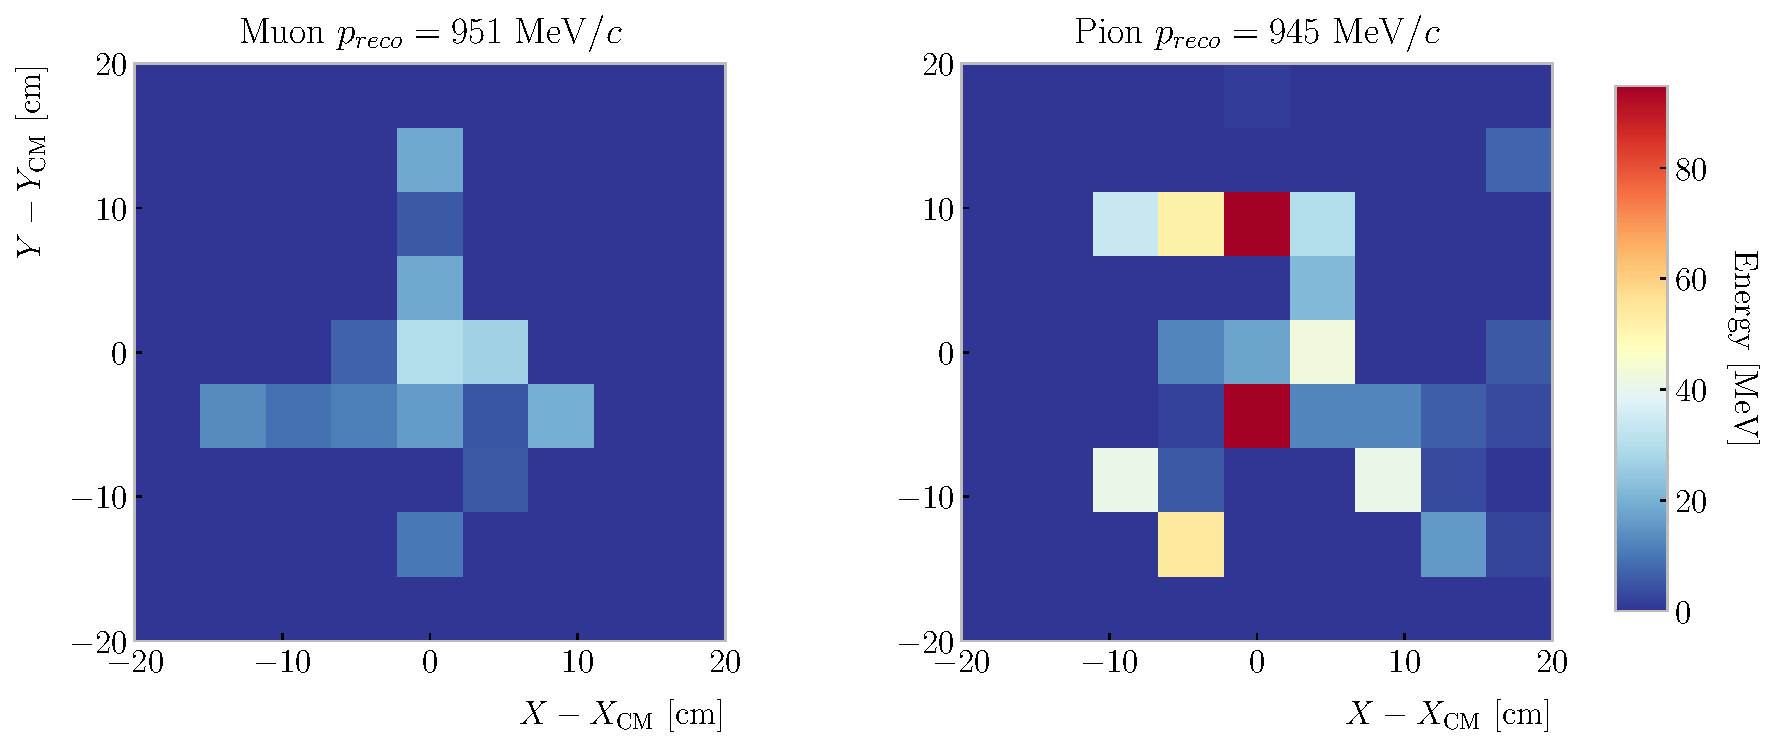
\includegraphics[width=.95\linewidth]{Images/GArSoft_PID/BDT/ecal_energy_distribution_example.pdf}
	\caption[Distributions of energy deposits in the ECal for a muon and a charged pion with similar momenta.]{Distributions of energy deposits in the ECal for a muon (left panel) and a charged pion (right panel) with similar momenta. The energy is projected onto the plane perpendicular to the principal component of the hits, and the positions are relative to the center of the interaction.}
	\label{fig:ecal_example}
\end{figure}

\subsection{Track-ECal matching}

One of the main players in the muon and pion separation is the way we associate clusters in the ECal to reconstructed tracks in the TPC. Missing some associations or making wrong ones can bias the ECal quantities that we can use for classifying particles. The current algorithm in GArSoft provides precise associations, i.e. most of the associations that it produces are correct, but it appears to miss an important number of associations (at least when using the default configuration).

The current TPC track-ECal cluster association algorithm is divided in four parts. It first checks whether the track end point fulfils certain conditions to be extrapolated. There are two cut values in this step, one for the drift direction and other radial.

If the point can be extrapolated, the code computes the coordinates of the centre of curvature using the Kalman fit estimates at the track end $(y, \ z, \ 1/R, \ \phi, \ \mathrm{tan}\lambda)$. It then compares the distance between this and the cluster in the $(z,y)$ plane with $R$. This introduces another cut in the perpendicular direction.

The next step is different for clusters is in the barrel or in one of the end caps. If it is a barrel cluster the algorithm extrapolates the track up to the radial distance of the cluster. There are three possible outcomes, the extrapolated helix can cut the cylinder of radius $r_{clus}$ two, one or zero times. I get the cut point that is closer to the cluster and check that it is either in the barrel or the end caps. Computing the difference between the $x$ coordinates of the cluster and the extrapolated point, the module checks that this is not greater than a certain cut. If the cluster is in an end cap, I propagate the track up to the $x$ position of the cluster. Then, the algorithm computes the angle in the $(z,y)$ plane between the centre of curvature and the cluster, $\alpha$, and the centre of curvature and the propagated point, $\alpha'$. A cut is applied to the quantity $(\alpha-\alpha')R$.

If the cluster contains more than a certain number $N$ of hits, I apply an extra cut to the dot product of the direction of the track at the propagated $x$ value and the cluster direction.

The code makes sure to only associate one end of the track (if any) to a cluster. However, it can associate more than one track to the same cluster. This makes sense, as different particles can contribute to the same cluster in the ECal, but it makes it difficult to quantify the relative contributions of the tracks to a certain cluster.

As a way of comparing the performance of this algorithm, a new, simpler association module was written. The goal was to have a simple and robust algorithm, which depends on as few parameters as possible and that can produce a one-to-one matching between tracks and ECal clusters.

\begin{figure}[t]
	\begin{subfigure}{0.5\textwidth}
		\centering
		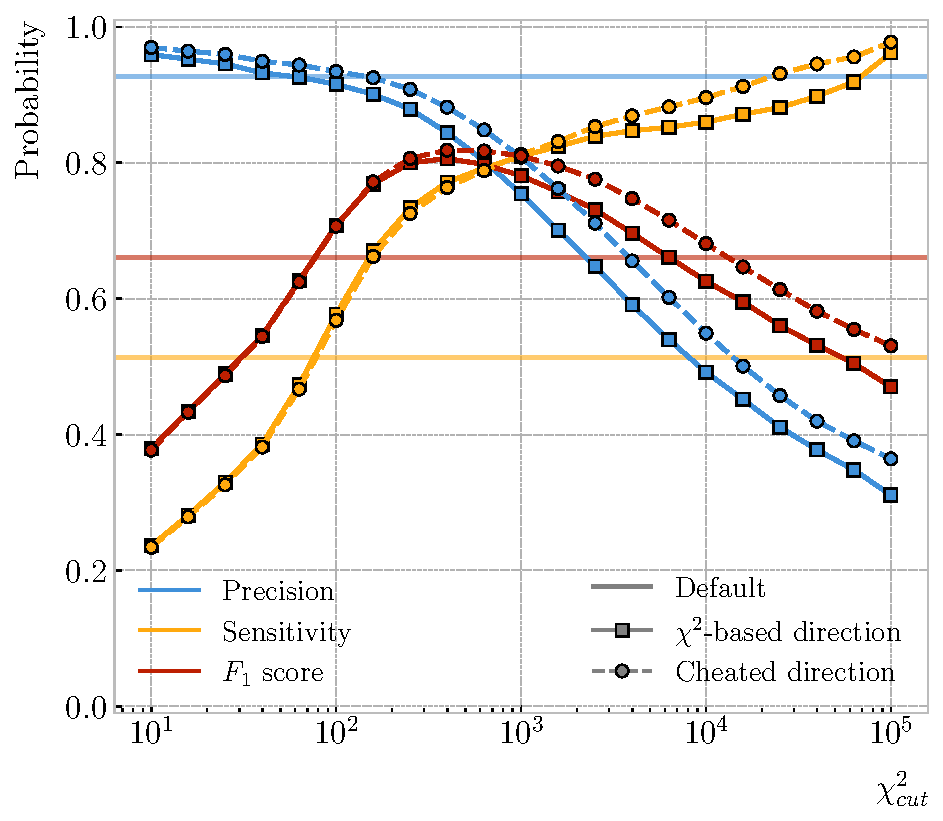
\includegraphics[width=.90\linewidth]{Images/GArSoft_PID/associations/helix_propagation_metrics_no_t0.pdf}
	\end{subfigure}
	\begin{subfigure}{0.5\textwidth}
		\centering
		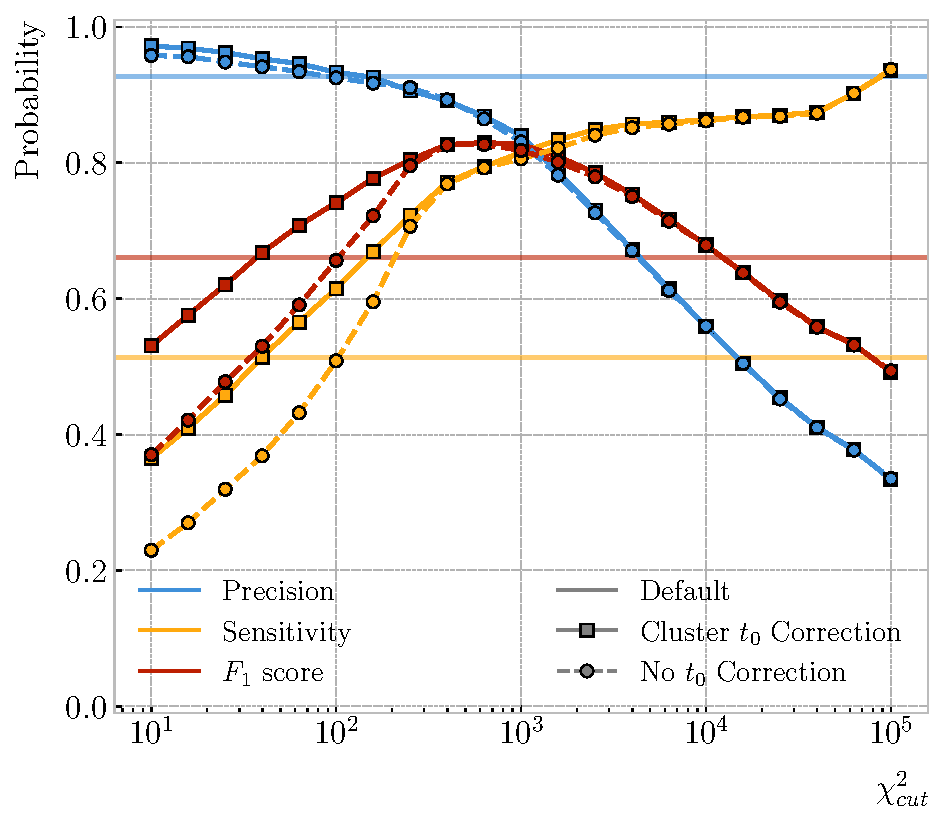
\includegraphics[width=.90\linewidth]{Images/GArSoft_PID/associations/helix_propagation_metrics_ecal.pdf}
	\end{subfigure}
	\caption{Left panel: comparison between the precision (blue), sensitivity (yellow) and $F_{1}$ score (red) obtained for the default (horizontal lines) and new algorithms, both with the $\chi^{2}$-based direction estimator (squares) and cheating the directions (circles), for different values of the $chi^{2}$ cut. Right panel: comparison of the performance of the new algorithm when applying the cluster $t_{0}$ correction (squares) and when (circles).}
	\label{fig:associations}
\end{figure}

For each reconstructed track, the new algorithms applies the same procedure to the forward and the backward fits irrespective of their end point positions. It first gets the Kalman fit parameters at the corresponding end point together with the $X$ position, $x_{0}$, $(y_{0}, \ z_{0}, \ 1/R, \ \phi_{0}, \ \mathrm{tan}\lambda)$.

For each ECal cluster, I compute the radial distance to the centre of the TPC and find the $\phi$ value in the range $[\phi_{0}, \ \phi_{0}+\mathrm{sign}(R)\phi_{max})$ that makes the propagated helix intersect with the circle defined with such radius. The $(x,y,z)$ position of the helix for the $\phi$ value found (if any) is then computed. In case there are two intersections, I keep the one that minimises the distance between $(y, z)$ and $(y_{c}, z_{c})$.

\begin{comment}
Figure \ref{fig:associations} (left panel) shows an example track (red line) being propagated up to $\phi_{0}+\mathrm{sign}(R)\pi/2$ (dashed blue line). The image also shows the ECal clusters present in the event (green squares). For each of them, the algorithm will try to find the intersections of the propagated helix and the circles defined with their corresponding radii.
\end{comment}

I then calculate $\chi^{2}$ value based on the Euclidean distance between the propagated point and the cluster:
\begin{equation}
	\chi^{2}/ndf = \frac{\sum_{n=0}^{2}\left(x^{(n)}-x^{(n)}_{c}\right)^{2}}{3}.
\end{equation}
If there was no intersection I store a $-1$ instead. In the end, for each reconstructed track in the event one ends up with two collections of $\chi^{2}$ values, one for each ECal cluster and fit directions.

The current code only supports having ECal clusters associated to one end of each track. We have two options to decide what track end to keep. The first one tries to cheat the selection, looking at the distance between the two track ends and the true start position of the associated MC particle. The second one keeps the track end with more $\chi^{2}$ entries below the cut.

This feature of only considering one track end limits the algorithm, making it not suitable for reconstructing events with particles originating outside the TPC. However, as for the moment the main concern of the group is the study of neutrino interactions off the gaseous argon, this is an acceptable assumption.

In order to associate a cluster to a track, I take all clusters with a $\chi^{2}$ value in the range $[0, \chi^{2}_{cut})$. If a cluster has been assigned to more than one track we leave it with the one with the lowest $\chi^{2}$.

This default behaviour of the algorithm can be modified to associate more than one track to each cluster. Not only that, but the $\chi^{2}$ values can be used to assign relative weights to the different contributions.

To evaluate the performance of the association method, I use a binary classification approach. In this case, I check the leading MC Track IDs associated to the reconstructed tracks and ECal clusters. I count an association as true positive (TP) if both Track IDs coincide. An association is considered false positive (FP) when the Track IDs are different. If a cluster has not been associated to any track but it shares the Track ID with a reconstructed track it is counted as a false negative (FN).

For the testing, I used a sample of 10000 FHC neutrino events inside the HPgTPC. Figure \ref{fig:associations} (left panel) shows the precision (blue line), sensitivity (yellow line), and $F_{1}$ score (red line) I obtained for different values of $\chi^{2}_{cut}$. For comparison, the same metrics computed for the default algorithm with the current configuration are also shown (dashed lines). In the case of the new algorithm, I used both the $\chi^{2}$-based method to estimate the track direction described earlier (square markers) and the cheated direction from the Geant-level information (circle markers). For either of these we achieve similar values of the precision compared to the old code, while having a considerably higher sensitivity. It can be seen that cheating the direction of the tracks only makes a difference at high $\chi^{2}_{cut}$, past the optimal value of the cut around the $F_{1}$ score maximum. Therefore, I set the $\chi^{2}$ method as the default.

\begin{figure}[t]
	\centering
	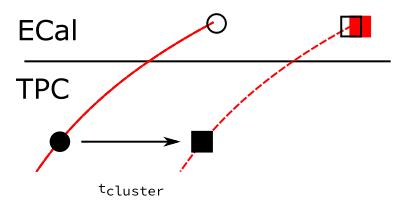
\includegraphics[width=.55\linewidth]{Images/GArSoft_PID/associations/drift_correction.png}
	\caption{Schematics of a possible option to deal with track-ECal associations in non-zero $t_{0}$ neutrino interaction events, trying to correct for the drift direction uncertainty in a cluster-by-cluster basis using the cluster time, $t_{cluster}$.}
	\label{fig:associations_drift}
\end{figure}

One of the possible weak points of this approach is that it relies on the position along the drift direction to make the decisions. Within the current ND-GAr design implemented in GArSoft, the timing information is provided by the ECal. That effectively means that prior to make the track-ECal associations the reconstructed $x$ positions of the track trajectories differ from the simulated ones by an amount:
\begin{equation}
	x_{reco}^{(n)} - x_{sim}^{(n)} = v_{drift} \ t_{0},
\end{equation}
where $v_{drift}$ is the mean drift velocity in our medium and the initial time is in the range $t_{0}\in[0, t_{spill})$ where $t_{spill}$ is the spill length. For a $10 \ \mu\mathrm{s}$ spill this translates into a maximum $30 \ \mathrm{cm}$ uncertainty on the drift direction position.

The current default in GArSoft sets $t_{0} = 0$, but the functionality to randomly sample this within the spill time is in place. Therefore, we need to understand what is the impact of a non-zero $t_{0}$ on the associations algorithm and foresee possible ways of minimising a loss in performance.

\begin{comment}
Figure \ref{fig:associations_drift} represents two different options to tackle the associations problem when having events with a non-zero initial time $t_{0}$. The circles represent the original points, whereas the squares indicate the corrected positions. The end points of the track and the propagated points up to the cluster radius are indicated using filled and unfilled markers respectively. The red square represents the position of the cluster.

In the first option (left panel) I try to correct for the drift coordinate position using the time associated to the cluster. Assuming that the drift time is much larger than the propagation time, $t_{cluster}$ could be used as a good estimation of the $t_{0}$. An alternative can be using the earliest time associated to a hit in said cluster. Doing this for each cluster before computing the $\chi^{2}$ value could be used as an alternative to knowing the specific value of the $t_{0}$, as when the association is correct this will provide the right correction but its impact is small enough to not change the position significantly in the case the cluster does not correspond to a given track.

The second method depicted in Fig. \ref{fig:associations_drift} (right panel) tries to propagate three different helices for each reconstructed track and fit direction. One is the original, uncorrected helix and the other two are obtained by adding factors of $\pm t_{spill}/2$ when computing the drift coordinate position. In this case one would compute a set of $\chi^{2}$ values for each helix, keeping in the end the collection that manages to keep more values below $\chi^{2}_{cut}$. An alternative approach could be using a family of helices instead, using uniformly sampled time correction values in the $\pm t_{spill}/2$ range.

Both options could offer a solution to the $t_{0}$ problem, and still need to be explored.
\end{comment}

Figure \ref{fig:associations_drift} represents a possible option to tackle the association problem when having events with a non-zero initial time $t_{0}$. The black and white circles represent the original points, whereas the squares indicate the corrected positions. The end points of the track and the propagated points up to the cluster radius are indicated using filled and unfilled markers respectively. The red square represents the position of the cluster.

Here I try to correct for the drift coordinate position using the time associated to the cluster. Assuming that the drift time is much larger than the propagation time, $t_{cluster}$ could be used as a good estimation of the $t_{0}$. An alternative can be using the earliest time associated to a hit in said cluster. Doing this for each cluster before computing the $\chi^{2}$ value could be used as an alternative to knowing the specific value of the $t_{0}$, as when the association is correct this will provide the right correction but its impact is small enough to not change the position significantly in the case the cluster does not correspond to a given track.

\begin{figure}[t]
	\centering
	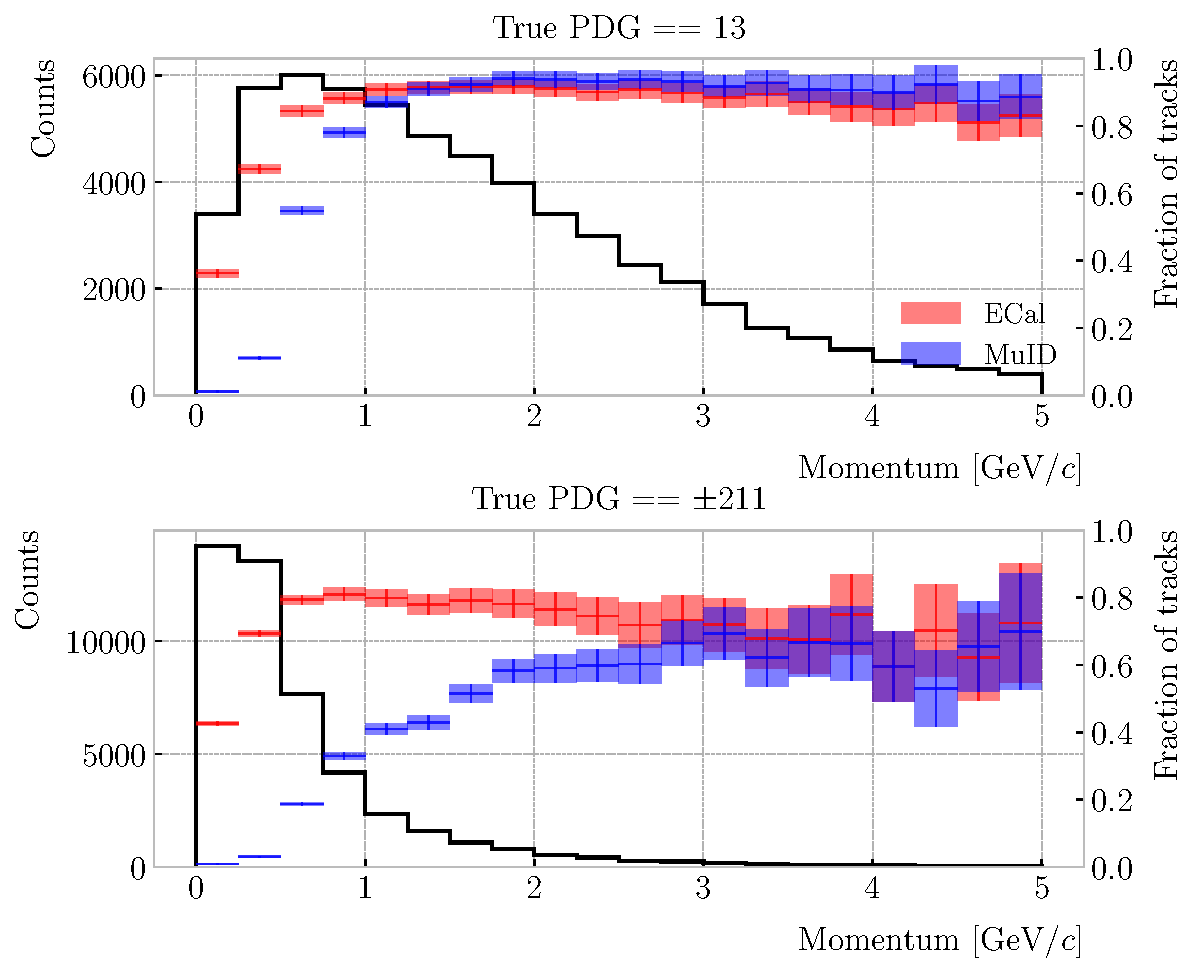
\includegraphics[width=.80\linewidth]{Images/GArSoft_PID/BDT/fraction_vs_preco_no_duplicates.pdf}
	\caption{Momentum distribution for the reconstructed muons (top panel) and charged pions (bottom panel) in a FHC neutrino sample, together with the fraction of them reaching the ECal (red) and MuID (blue). Each entry corresponds to a reconstructed track, backtracked to a true muon or pion which has not produced any other reconstructed track.}
	\label{fig:fraction_particles_ecal_muid}
\end{figure}

I tested the effect of this correction again using a sample of 10000 FHC neutrino events. Figure \ref{fig:associations} (right panel) shows the precision (blue line), sensitivity (yellow line), and $F_{1}$ score (red line) for the case the cluster $t_{0}$ correction is applied (square markers) and for the no correction case (circle markers), as a function of $\chi^{2}_{cut}$. In this case, the differences are particularly notorious at low values of the cut. It makes sense, as the $t_{0}$ effect becomes subdominant when the distance we consider grows large. Overall, the correction increases the sensitivity while keeping the precision almost unchanged. As a result, I apply the $t_{0}$ correction to the generated samples as the default.

\subsection{Classification strategy}

\begin{figure}[t]
	\centering
	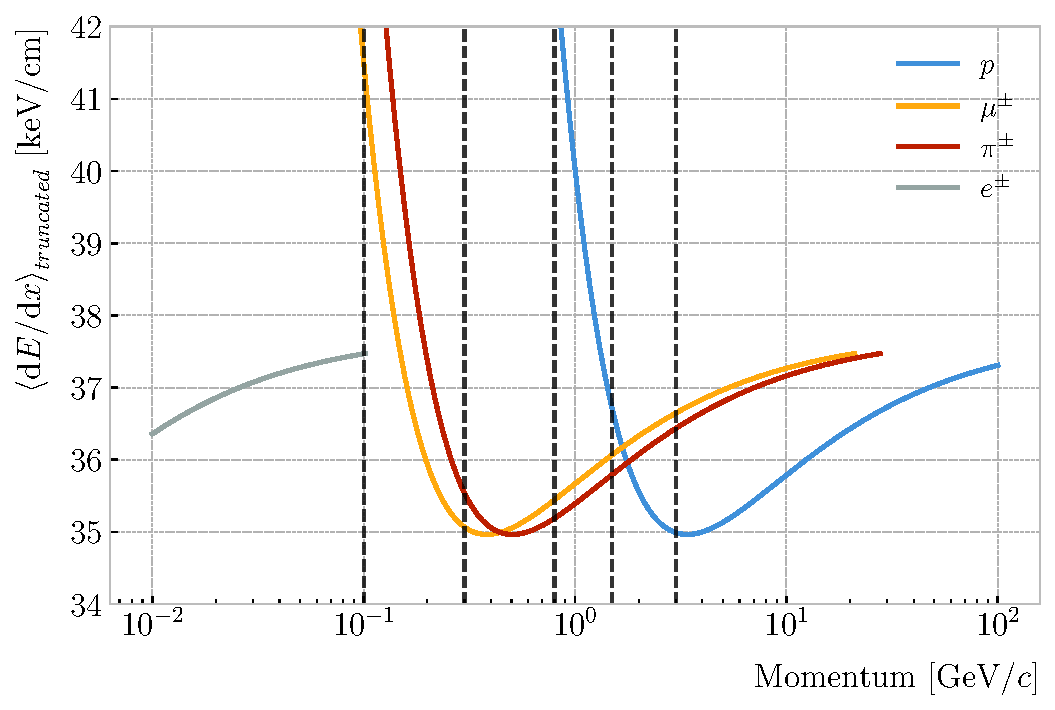
\includegraphics[width=.80\linewidth]{Images/GArSoft_PID/BDT/dEdx_fit_only.pdf}
	\caption{Predicted truncated mean $\mathrm{d}E/\mathrm{d}x$ versus momentum, for electrons, muons, charged pions and protons, obtained using the \gls{aleph} parametrisation. The vertical dashed lines represent the boundaries of the six regions used for the muon and pion classification training.}
	\label{fig:dEdx_vs_momentum_regions}
\end{figure}

The problem of the muon and charged pion separation has to be viewed in the broader context of the particle identification in our detector. Focusing on the beam neutrino interactions, it is clear that we are going to have muons and pions spanning a broad momentum range. Not only that, but we will also have other particles with similar characteristics that will make the classification even more challenging. Therefore, we are presented with a task that will depend heavily on the kinematic range we are looking at each time, as both the available information and the possible impurities of other particle species vary.

For instance, distinguishing muons from pions could be difficult at low momenta, as a great number of them do not reach the ECal. Therefore, we could think of tailoring a version of the classification for that particular case, which could be complemented with a $\mathrm{d}E/\mathrm{d}x$ measurement. Likewise, for momenta $\gtrsim 1~\mathrm{GeV}$ muons and pions reach the calorimeters efficiently, but so do protons. Because of this, one can try to train another classifier for this energy range, and rely on other methods to remove as many of the protons as possible.

Figure \ref{fig:fraction_particles_ecal_muid} shows the momentum distribution of the reconstructed muons (top) and pions (bottom) in a FHC sample. It also contains the fraction of particles reaching the ECal (red) and MuID (blue), for the different momentum bins. In Fig. \ref{fig:dEdx_vs_momentum_regions} I show the mean $\mathrm{d}E/\mathrm{d}x$ of different particles as a function of the momentum, computed using the \gls{aleph} parametrisation with the best fit parameters found in Subsec. \ref{subsec:mean_dEdx}.

Using these two figures as references, I decided to approach the classification by dividing the problem into six different momentum regions. A summary of these can be found in Tab. \ref{tab:bdt_regions}. The basic idea is to exploit all the information that is available in each region and . For the problem at hand, I prepared separated samples of isotropic single muons and pions, with momenta uniformly distributed along the corresponding momentum range. Each sample contains $50000$ events of the corresponding particle species. I did not generate samples for the first region, as it is assumed that the separation can be achieved using $\mathrm{d}E/\mathrm{d}x$ only. For the last region, I generated particles up to a momentum of $10~\mathrm{GeV}/c$, as that is well above the typical energies of muons and pions from FHC neutrino interactions in ND-GAr.

Additionally, I prepared another sample of $100000$ FHC neutrino events. For each interaction, I select the reconstructed particles which were backtracked to true muons or charged pions. I use this dataset to perform validation checks, to see how the models trained with the single particle data generalise to a more realistic scenario.

\begin{table}[t]
	\caption{Momentum ranges and description of the PID approach assumed for the muon and pion classification task.}
	\begin{center}
		\begin{small}
			\begin{tabular}{p{2.7cm}|l}
				Momentum range                                    & Description                                                                          \\[1mm] \hline \rule{0pt}{1.1\normalbaselineskip}
				$< 0.1$ \hfill $\mathrm{GeV}/c$      & All tracks can be separated with $\mathrm{d}E/\mathrm{d}x$                           \\[2mm]
				$[0.1,~0.3)$ \hfill $\mathrm{GeV}/c$ & Use ECal for reaching muons and pions, $\mathrm{d}E/\mathrm{d}x$ for the rest        \\[2mm]
				$[0.3,~0.8)$ \hfill $\mathrm{GeV}/c$ & Use ECal for muons and pions, $\mathrm{d}E/\mathrm{d}x$ for protons                  \\[2mm]
				$[0.8,~1.5)$ \hfill $\mathrm{GeV}/c$ & Use ECal and MuID for muons and pions,  $\mathrm{d}E/\mathrm{d}x$ for protons        \\[2mm]
				$[1.5,~3.0)$ \hfill $\mathrm{GeV}/c$ & Use ECal and MuID for muons and pions, ToF for protons                               \\[2mm]
				$\geq 3.0$ \hfill $\mathrm{GeV}/c$   & Use ECal and MuID for muons and pions, $\mathrm{d}E/\mathrm{d}x$ and ToF for protons
			\end{tabular}
		\end{small}
	\end{center}
	\label{tab:bdt_regions}
\end{table}

To tackle this classification problem, I make use of Boosted Decision Trees (\gls{bdt}). A decision tree uses a flowchart-like structure to make decisions based on some input data. It starts from a root node, which represents the complete dataset, and then it splits this based on the variable or feature which gives the best separation between classes, creating two new nodes. The process repeats for each node until it reaches a certain limit, like a maximum number of splits or some tolerance criteria. The last set of nodes are often called leave nodes, and represent the final prediction of the classifier.

Boosting refers to a family of methods to combine the predictions from multiple classifiers, following a sequential approach where each new model learns from the errors of the previous one. The process starts with a simple decision tree, which is used to make predictions on the training data. Then, the data points misclassified by the first model are assigned higher weights, and another decision tree is trained on the data with adjusted weights. The predictions of the two trees are then combined, and the cycle repeats for a predefined number of iterations. Gradient boosting uses the direction of the steepest error descent to guide the learning process and improve the accuracy with each iteration.

\subsection{Feature selection and importance}

Using the reconstructed tracks as a starting point, I compute a number of ECal and MuID variables for each of them. As there can be more than one cluster associated to a track, what I do is collect all associated clusters and compute these variables from the complete collection of associated hits. For the MuID, because it only features three layers and typically there will be less hits, I also allow single hits to be associated with tracks\footnote{At the reconstruction level what happens is that non-clustered hits are put into single hit clusters, instead of being thrown away. This is necessary to keep the consistency of the track-cluster association code.}. I can roughly divide the variables in three types: energy-related, geometry-related and statistical. In the following, I briefly describe the variables related exclusively to the ECal:

\begin{itemize}
	\item \textbf{Energy-related ECal}
	\begin{itemize}
		\item ECal total energy (ClusterTotalEnergy): sum of the energy of all the ECal hits.
		\item Mean ECal hit energy (HitMeanEnergy): mean of the hit energy distribution.
		\item Standard deviation ECal hit energy (HitStdEnergy): standard deviation of the hit energy distribution.
		\item Maximum ECal hit energy (HitMaxEnergy): maximum of the hit energy distribution.
	\end{itemize}
	\item \textbf{Geometry-related ECal}
	\begin{itemize}
		\item Mean distance hit-to-cluster (DistHitClusterMean): mean of the distance distribution between the hits and the corresponding cluster's main axis.
		\item RMS distance hit-to-cluster (DistHitClusterRMS): root mean square of the distance distribution between the hits and the corresponding cluster's main axis.
		\item Maximum distance hit-to-centre (DistHitCenterMax): maximum of the distance distribution between the hits and the centre of the TPC.
		\item Time-of-Flight velocity (TOFVelocity): slope obtained when fitting a straight line to the hit time versus hit distance to the centre (i.e. $d = v \times t$).
	\end{itemize}
	\item \textbf{Energy and geometry ECal}
	\begin{itemize}
		\item Radius 90\% energy (Radius90E): distance in the hit-to-cluster distribution for which 90\% of the total energy is contained in the hits that are closer to the axis (i.e. radius that contains 90\% of the energy).
	\end{itemize}
	\item \textbf{Statistical ECal}
	\begin{itemize}
		\item Number of hits (NHits): total number of hits associated to the track.
		\item Number of layers with hits (NLayers): not really a count of all layers with hits but the difference between the last and the first layer with hits.
	\end{itemize}
\end{itemize}

\begin{figure}[p!]
	\centering
	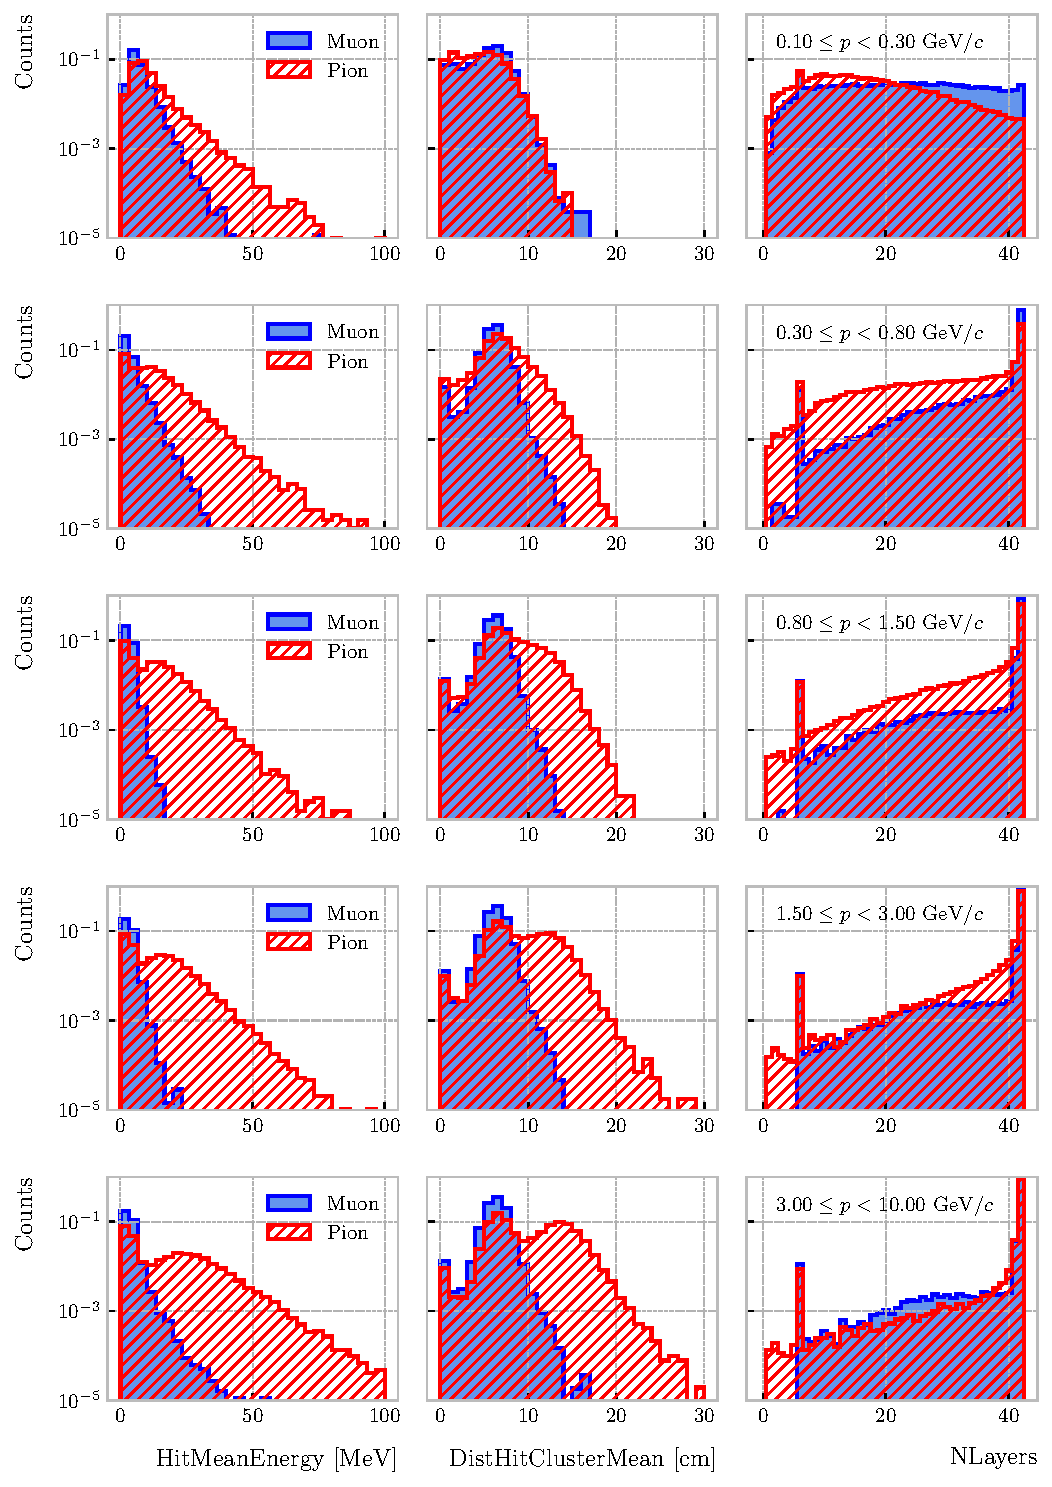
\includegraphics[width=.95\linewidth]{Images/GArSoft_PID/BDT/ecal_feature_distribution_all_example.pdf}
	\caption[Example ECal feature distributions for muons and charged pions in the five different momentum ranges considered.]{Example ECal feature distributions for muons (blue) and charged pions (red) in the five different momentum ranges considered (from top to bottom, in ascending momentum order). From left to right: mean hit energy, mean distance hit-to-cluster, and number of layers with hits.}
	\label{fig:ecal_feature_example}
\end{figure}

\begin{figure}[t]
	\centering
	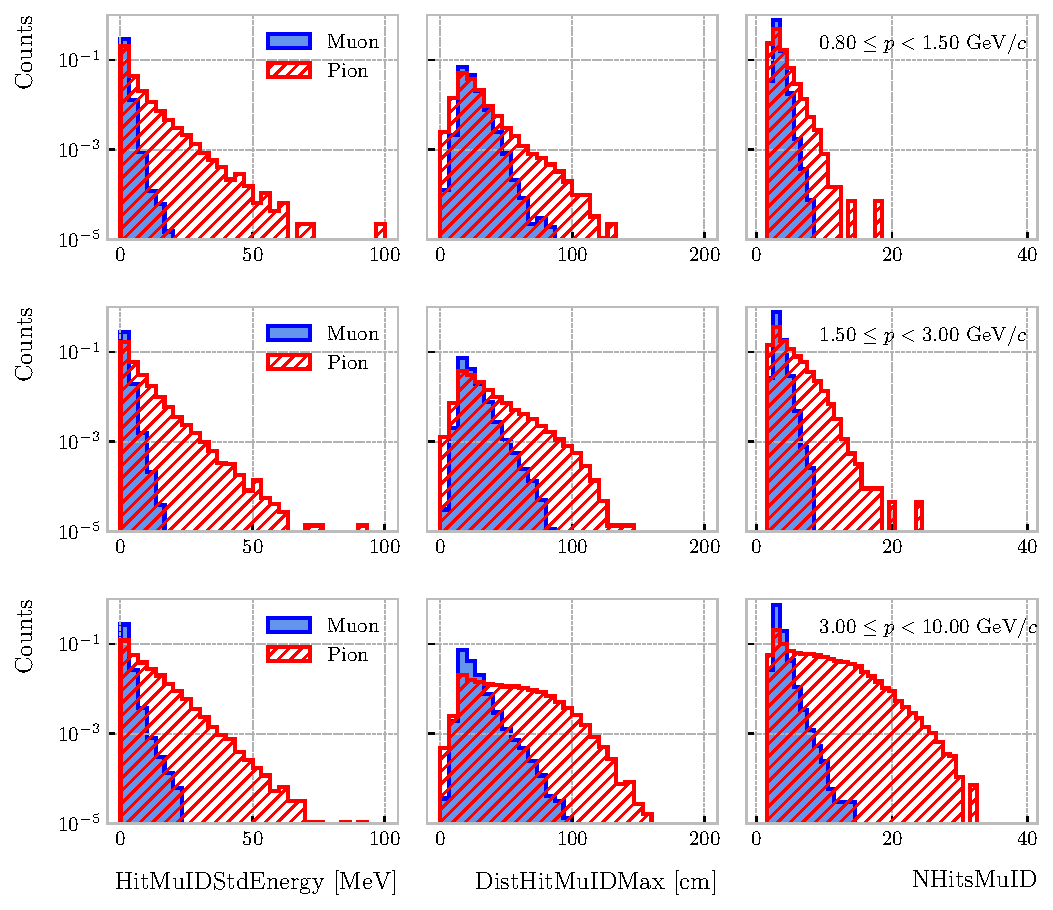
\includegraphics[width=.95\linewidth]{Images/GArSoft_PID/BDT/muid_feature_distribution_all_example.pdf}
	\caption[Example MuID feature distributions for muons and charged pions in the three different momentum ranges considered.]{Example MuID feature distributions for muons (blue) and charged pions (red) in the three different momentum ranges considered (from top to bottom, in ascending momentum order). From left to right: standard deviation hit energy, maximum distance hit-to-hit, and number of hits.}
	\label{fig:muid_feature_example}
\end{figure}

Figure \ref{fig:ecal_feature_example} shows the distributions of three different ECal variables, separating true muons (blue) and charged pions (red), for the five momentum ranges considered. I chose to show one feature from each category, namely the mean energy per hit (left column), the mean distance between the hits and the centre of the cluster (middle column), and the number of ECal layers with hits (right column). These give an idea of the separating power of the different features, and how it changes considerably with the energy. In the number of layers with hits distributions, the peak at $6$ is due to the fact that the first six ECal layers sit inside the pressure vessel\footnote{Note to self: check this. I thought the ECal barrel had 8 layers of tiles, and that all of them were inside the pressure vessel.}. Therefore, some of the particles get stopped crossing it, never making it to the seventh layer.

In the case of the MuID, because at low momenta a significant fraction of the particles do not make it past the ECal, I only consider the information coming from this detector for momenta $\geq 0.8~\mathrm{GeV}/c$, i.e. for the last three momentum regions. The variables I extract from it are the following:
\begin{itemize}
	\item \textbf{Energy-related MuID}
	\begin{itemize}
		\item MuID total energy (ClusterMuIDTotalEnergy): sum of the energy of all the MuID hits.
		\item Mean MuID hit energy (HitMuIDMeanEnergy): mean of the MuID hit energy distribution.
		\item Standard deviation MuID hit energy (HitMuIDStdEnergy): standard deviation of the MuID hit energy distribution.
		\item Maximum MuID hit energy (HitMuIDMaxEnergy): maximum of the MuID hit energy distribution.
	\end{itemize}
	\item \textbf{Geometry-related MuID}
	\begin{itemize}
		\item Maximum distance MuID hit-to-hit (DistHitMuIDMax): maximum distance between pairs of MuID hits (not sure this is a good variable, distribution looks nuts).
		\item Maximum distance MuID hit-to-centre (DistHitCenterMuIDMax): maximum of the distance distribution between the MuID hits and the centre of the TPC.
	\end{itemize}
	\item \textbf{Statistical MuID}
	\begin{itemize}
		\item Number of hits (NHitsMuID): total number of MuID hits associated to the track.
		\item Number of layers with hits (NLayersMuID): not really a count of all layers with MuID hits but the difference between the last and the first layer with MuIDhits.
	\end{itemize}
\end{itemize}

Figure \ref{fig:muid_feature_example} shows the distributions of three different MuID variables, separating true muons (blue) and charged pions (red), for the three momentum ranges which use the muon tagger information. In this case I decided to  standard deviation of the MuID hit energy distribution (left column), the maximum distance between the MuID hit pairs (middle column), and the number of MuID hits (right column). These variables are used together with the ECal features at high momenta, providing additional disambiguation power.

\begin{figure}[t]
	\centering
	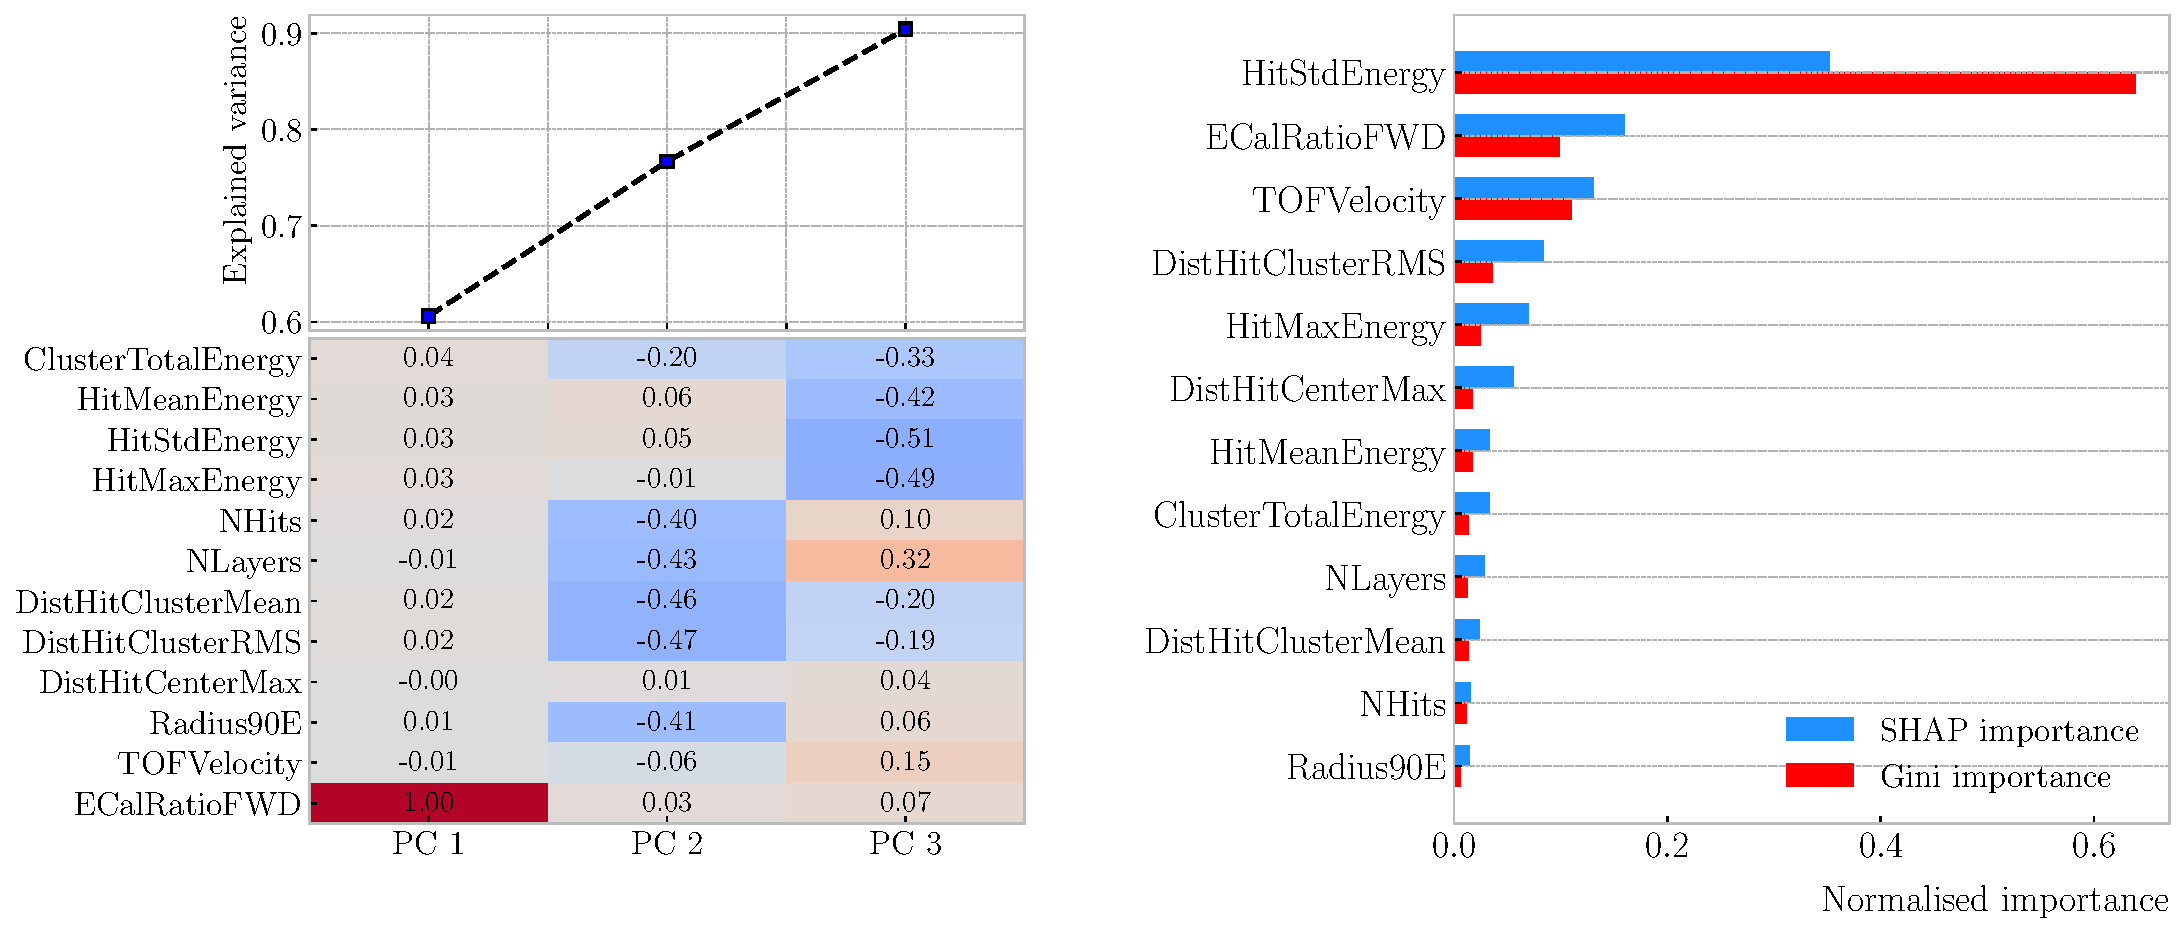
\includegraphics[width=.95\linewidth]{Images/GArSoft_PID/BDT/summary_pca_p0_0.55_sigmap_0.25.pdf}
	\caption{Left panel: cumulative explained variance for the first three principal components (top panel) and contribution of the different features to the principal axes in feature space (bottom panel). Right panel: Shapley (blue) and Gini (red) feature importances for the different input features. Both figures correspond to the samples in the momentum range $0.3 \leq p < 0.8 ~ \mathrm{GeV}/c$.}
	\label{fig:bdt_pca_importance_ii}
\end{figure}

\begin{figure}[t]
	\centering
	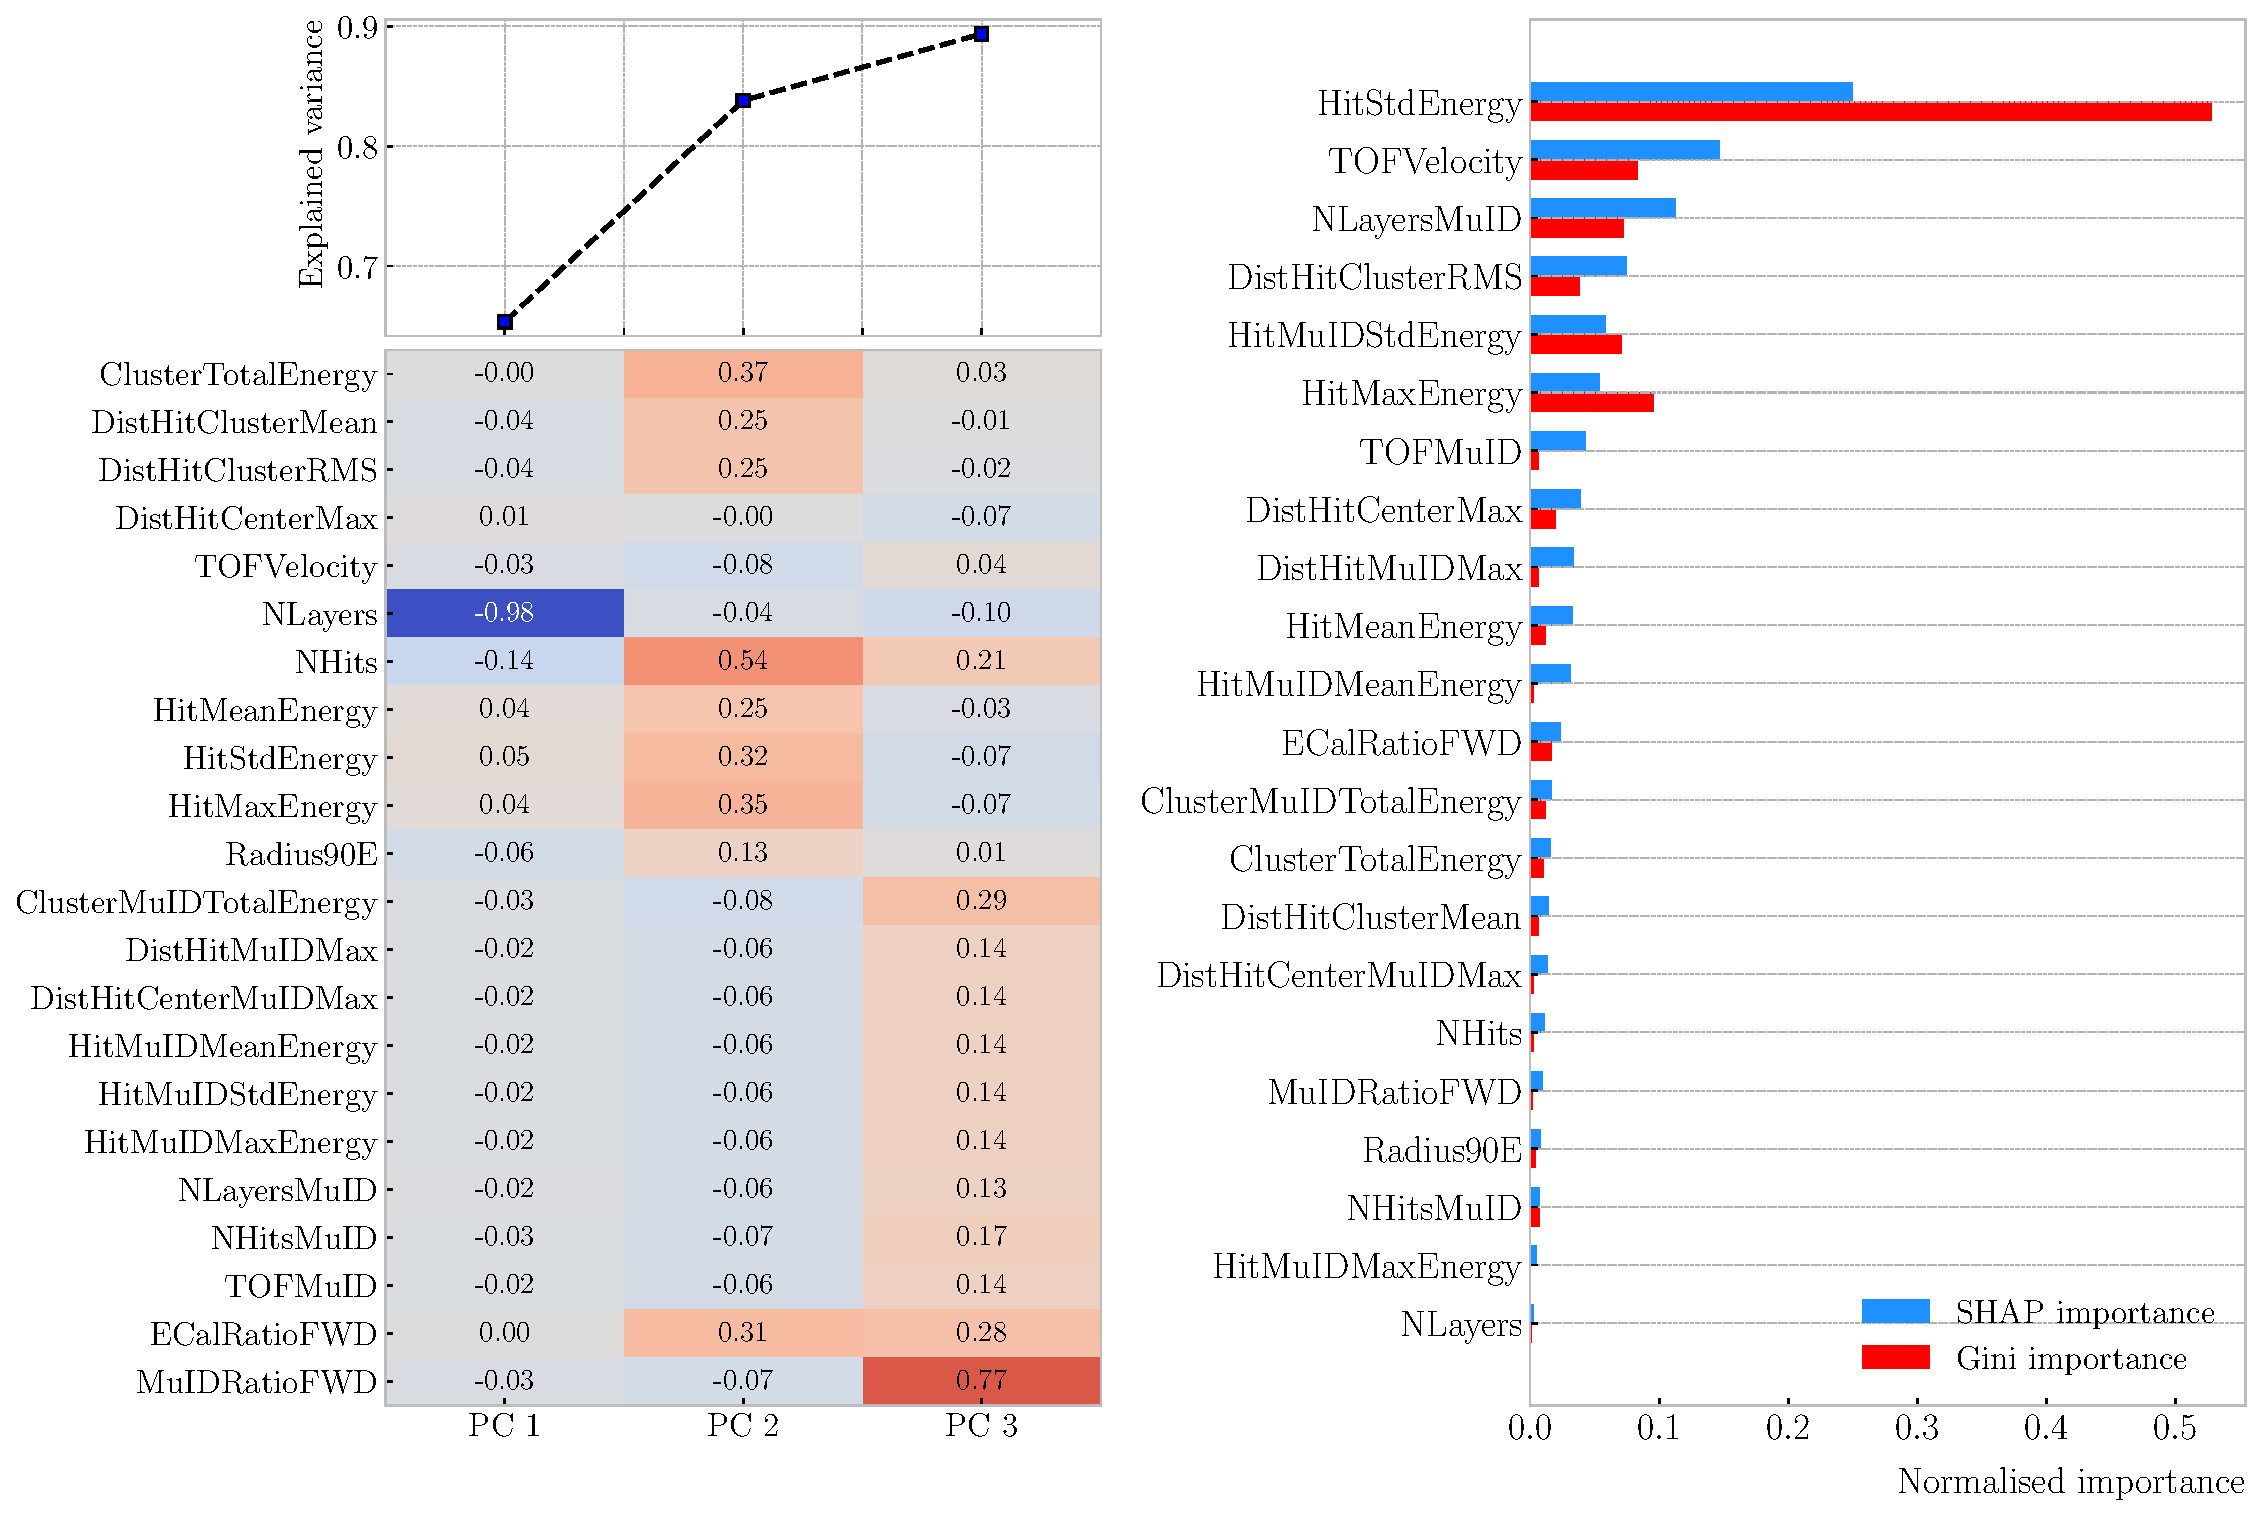
\includegraphics[width=.95\linewidth]{Images/GArSoft_PID/BDT/summary_pca_p0_1.15_sigmap_0.35.pdf}
	\caption{Left panel: cumulative explained variance for the first three principal components (top panel) and contribution of the different features to the principal axes in feature space (bottom panel). Right panel: Shapley (blue) and Gini (red) feature importances for the different input features. Both figures correspond to the samples in the momentum range $0.8 \leq p < 1.5 ~ \mathrm{GeV}/c$.}
	\label{fig:bdt_pca_importance_iii}
\end{figure}

\begin{comment}
\begin{figure}[t]
	\begin{subfigure}{0.32\textwidth}
		\centering
		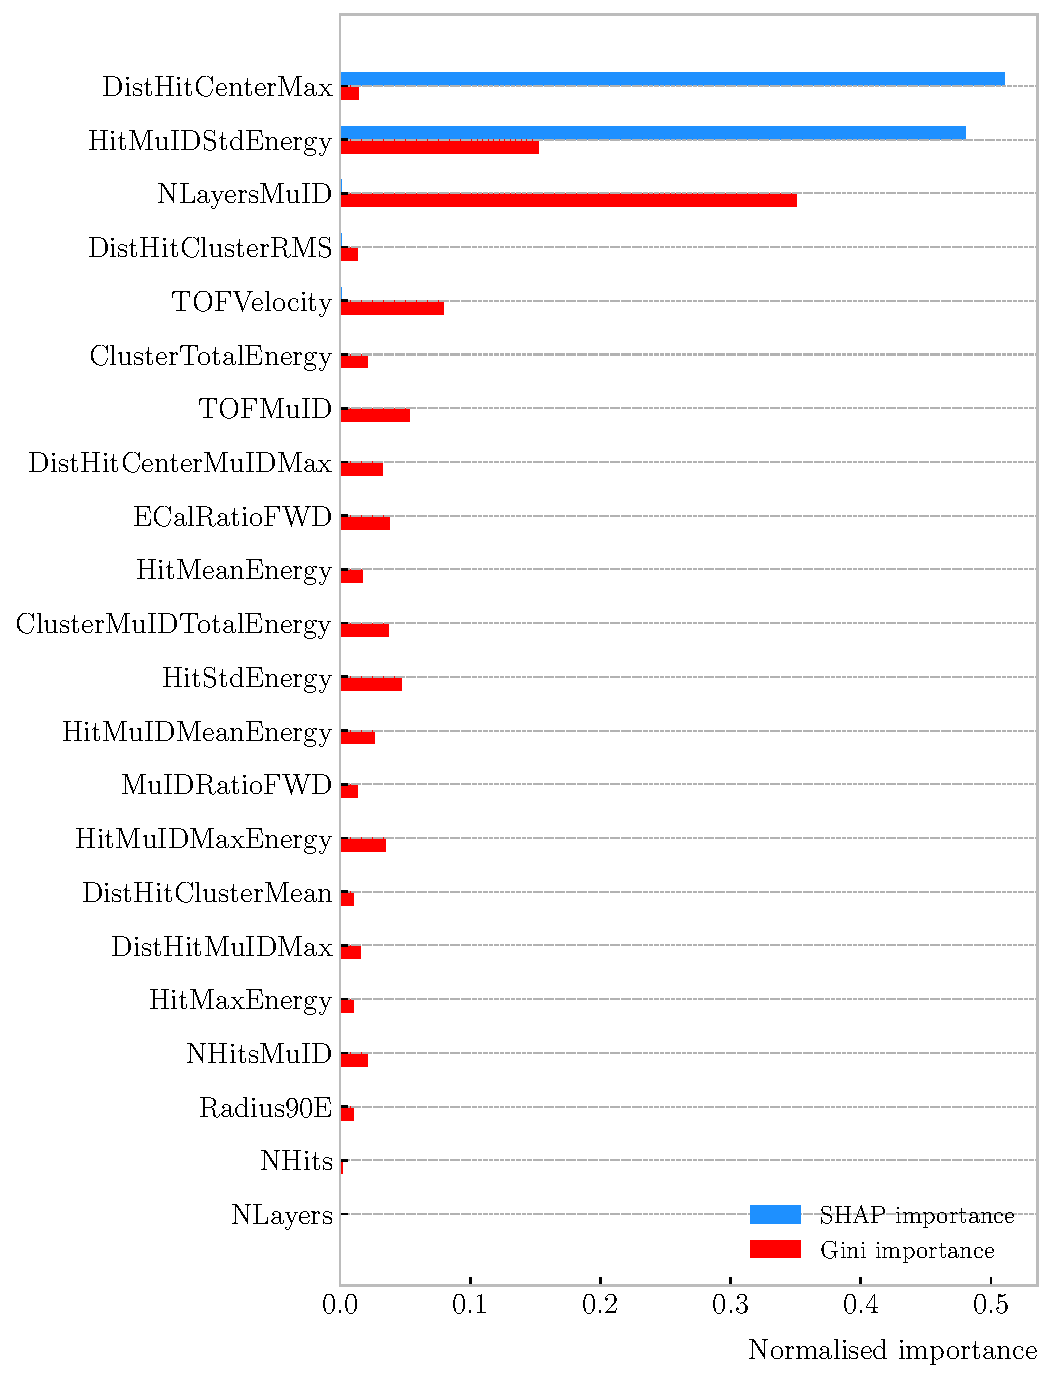
\includegraphics[width=.99\linewidth]{Images/GArSoft_PID/BDT/importance/feature_importance_p0_1.15_sigmap_0.35_MuID.pdf}
	\end{subfigure}
	\begin{subfigure}{0.32\textwidth}
		\centering
		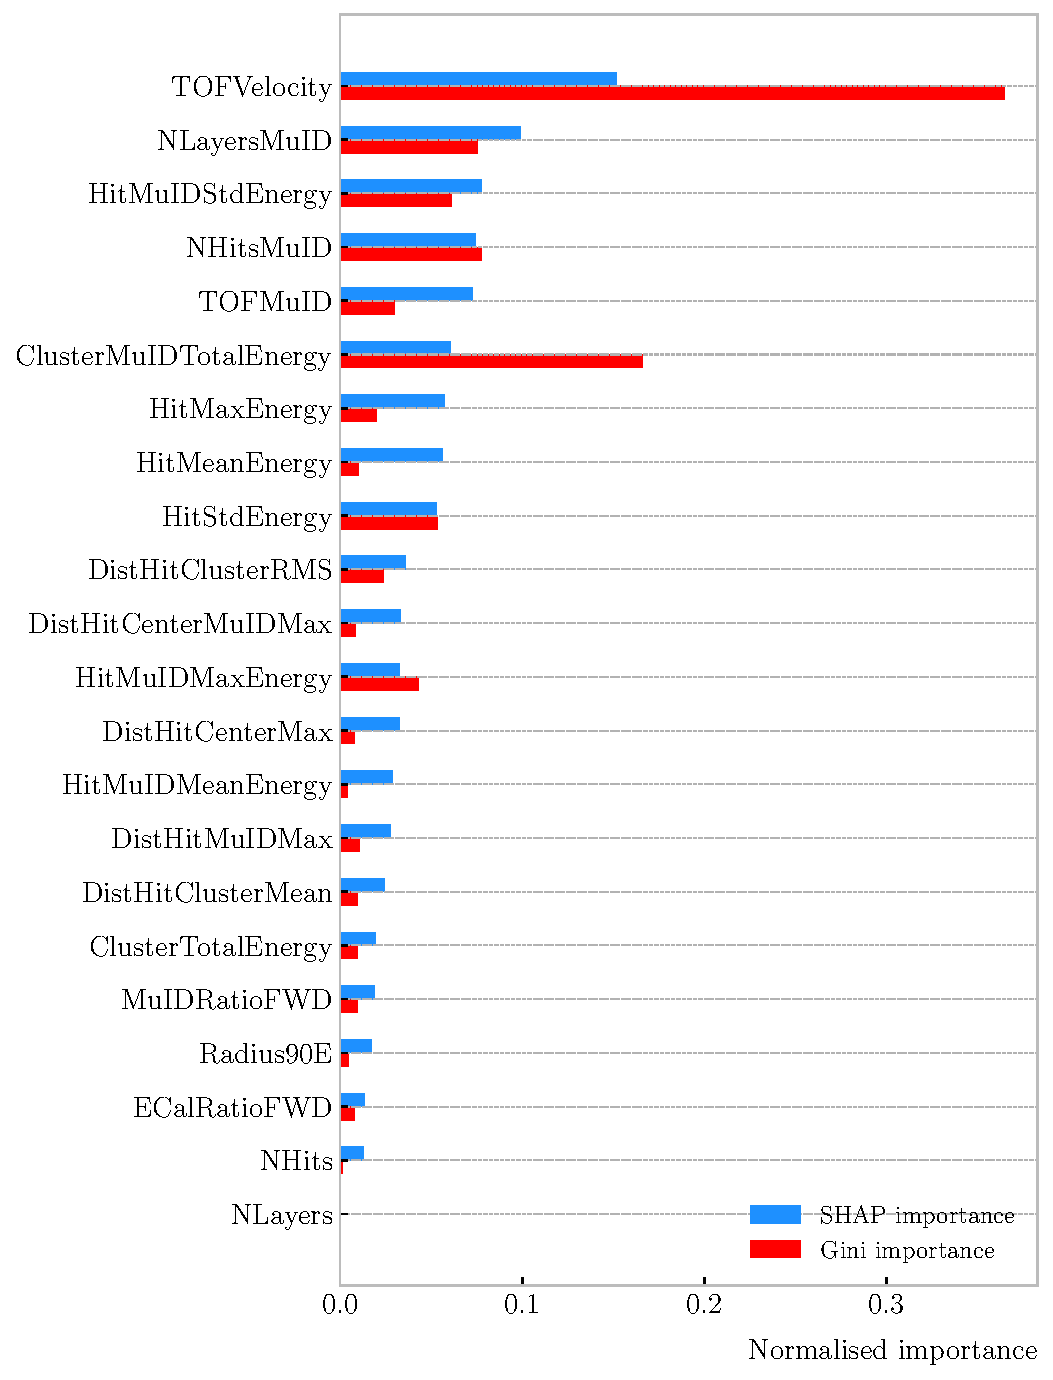
\includegraphics[width=.99\linewidth]{Images/GArSoft_PID/BDT/importance/feature_importance_p0_2.25_sigmap_0.75_MuID.pdf}
	\end{subfigure}
	\begin{subfigure}{0.32\textwidth}
		\centering
		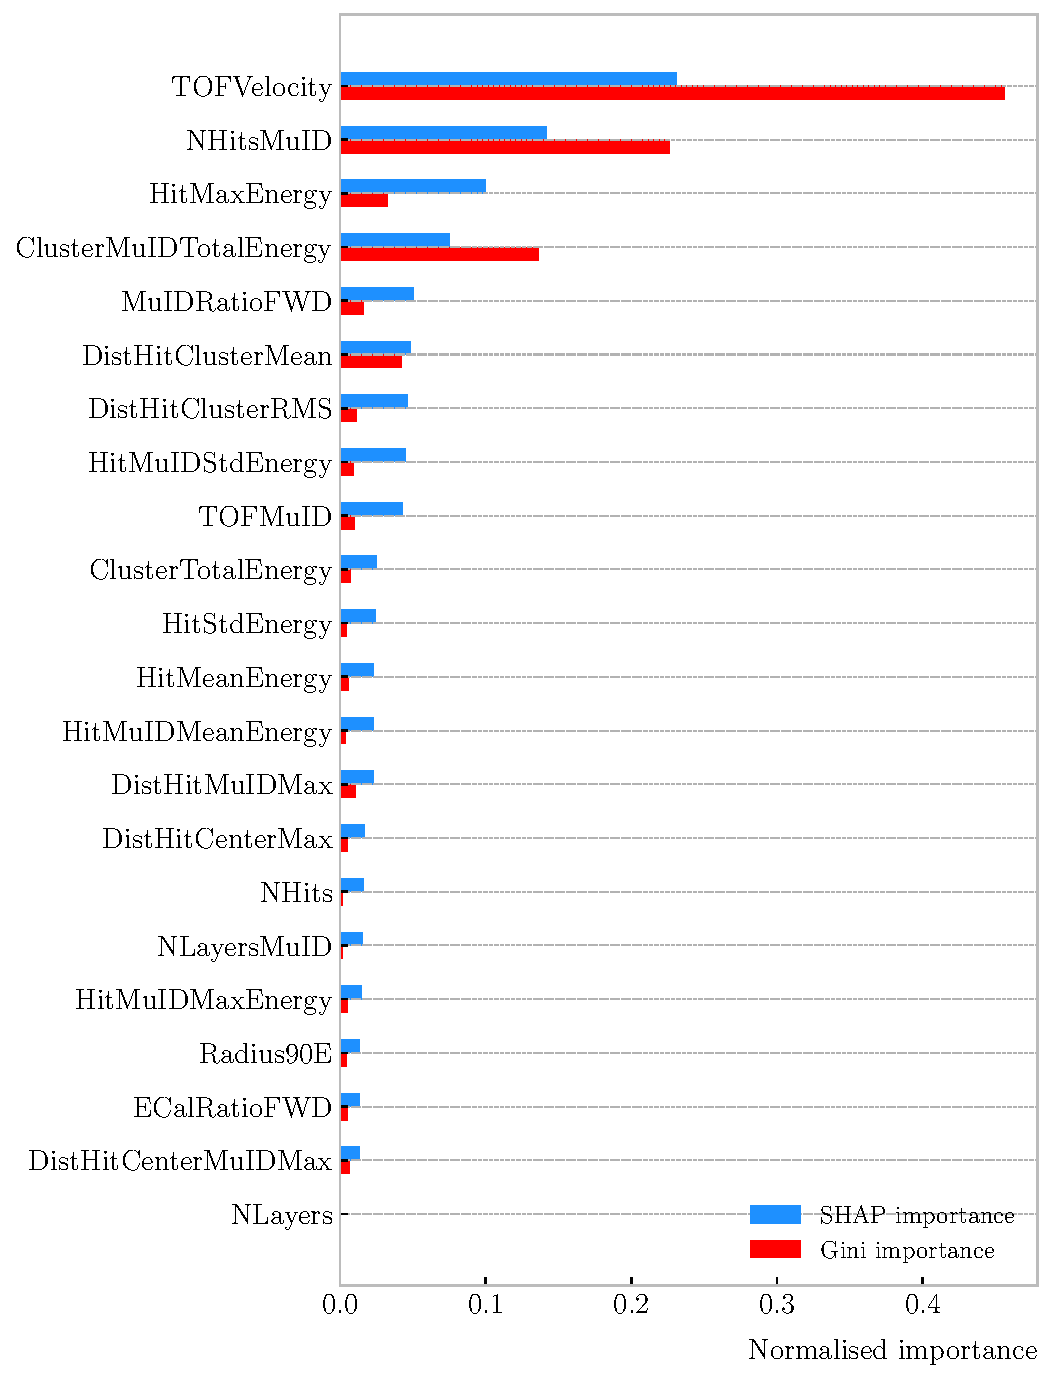
\includegraphics[width=.99\linewidth]{Images/GArSoft_PID/BDT/importance/feature_importance_p0_6.50_sigmap_3.50_MuID.pdf}
	\end{subfigure}
	\caption{Left panel: number of non-decaying, decaying and decaying in the fiducial volume pions for a MC sample of $10^{5}$, $p=500 \ \mathrm{MeV}$ isotropic positively charged pions inside the TPC. Right panel: event display for a positive pion decaying inside the fiducial volume, with a single reconstructed track for the pion and muon system.}
	\label{fig:pion_decays}
\end{figure}
\end{comment}

Once our features have been defined, one can do some exploratory analysis to understand how well the variables describe the target class, and avoid the black-box approach by what features are most relevant for the learning process. This way, I performed a feature analysis for each of the momentum ranges I divided this classification problem into. It follows three steps: first a principal component analysis (PCA), followed by a feature importance study using Gini and Shapley values, and finally a feature permutation importance analysis.

The PCA is useful to understand the variance of the feature space. It is an unsupervised machine learning technique that allows the user to perform a dimensionality reduction. It uses a singular value decomposition of the input features to project them into a lower dimensional space. The idea is to find the matrix $\mathbf{C}_{m}$, whose columns are the first $m$ orthonormal eigenvectors of the input covariance matrix. Consider the $n \times p$ real matrix of input data $\mathbf{X}$, where $n$ is the number of samples and $p$ the number of features. If $\mathbf{X}$ is centred, i.e. the means of its columns are equal to zero, we can write the covariance matrix of $\mathbf{X}$ as $\mathbf{C}=\mathbf{X}^{\intercal}\mathbf{X}/(n-1)$. This matrix can be diagonalised, yielding:
\begin{equation}
	\mathbf{C}=\mathbf{V}\mathbf{L}\mathbf{V}^{\intercal},
\end{equation}
where $\mathbf{V}$ is a matrix of eigenvectors and $\mathbf{L}$ a diagonal matrix with eigenvalues $\lambda_{i}$. Then, performing SVD on $\mathbf{X}$ gives us:
\begin{equation}
	\mathbf{X}=\mathbf{U}\mathbf{S}\mathbf{W}^{\intercal},
\end{equation}
where $\mathbf{U}$ is a unitary matrix, whose columns are called left singular vectors, $\mathbf{S}$ is a diagonal matrix of single values $s_{i}$, and $\mathbf{W}$ is another unitary matrix, its columns known as right singular vectors. This way, we can write:
\begin{equation}
	\mathbf{C}=\mathbf{W}\mathbf{S}\mathbf{U}^{\intercal}\mathbf{U}\mathbf{S}\mathbf{W}^{\intercal}/(n-1)=\mathbf{W}\frac{\mathbf{S}^{2}}{n-1}\mathbf{W}^{\intercal}.
\end{equation}
meaning that the right singular vectors are also the eigenvectors of the covariance matrix. The SVD can be computed numerically following an iterative approach.

This way, taking an input data vector $X \in \mathbb{R}^{n}$, the resulting feature vector $Y \in \mathbb{R}^{m}$ is given by:
\begin{equation}
	Y = \mathbf{C}_{m}^{\intercal} X.
\end{equation}
The new features capture most of the variance of the original sample, while being lower dimensional, as $m<n$.

Before applying the PCA reduction one needs to centre and scale the input data. Centring is necessary when using SVD to obtain the eigenvectors of the covariance matrix, as only in that case we can do the identification with the right singular vectors from the input data. Scaling is needed when variables are on different scales, as some can then dominate the PCA procedure.

I used the PCA module of \texttt{scikit-learn}, together with the \texttt{RobustScaler}, which centres the data and scales it based on the interquartile range. In Fig. \ref{fig:bdt_pca_importance_ii} (left panel) and Fig. \ref{fig:bdt_pca_importance_iii} (left panel) I show the results I obtained from the PCA for the momentum ranges $0.3 \leq p < 0.8 ~ \mathrm{GeV}/c$ and $0.8 \leq p < 1.5 ~ \mathrm{GeV}/c$, respectively. Notice that in the second case the number of features increases considerably, as this is the first region which uses the MuID variables. I found that, in all the cases, adding a fourth PC does not add additional information. As it can be seen in the top panels of the figures, the cumulative explained variance is already over $80\%$ with three PCs.

The bottom panels show the contribution of the variables to the principal axes. For the two first momentum regions, I observe a tendency of the energy-related and the geometry-related ECal variables to be clustered together. For the other ranges, when I include the MuID variables, there seems to be a division between ECal and MuID variables. For these, it seems like the number of ECal layers with hits also plays an important role.

The next step in the analysis is to quantify the importance of the features based on two additional metrics, namely the Gini and the Shapley values. The Gini importance, often called mean decrease impurity, is based on how much a feature contributes to the purity improvement at the splits in each decision tree. The purity is measured in terms of the Gini impurity index, defined as:
\begin{equation}
	I_{G} = 1 - \sum_{i} f_{i},
\end{equation}
where $f_{i}$ is the fractional abundance of the $i$-th class. Then, for each split one can compute the weighted decrease in impurity as:
\begin{equation}
	\Delta_{G} = \frac{N_{t}}{N} \left(I_{G} - \frac{N_{t}^{R}}{N_{t}} I_{G}^{R} - \frac{N_{t}^{L}}{N_{t}} I_{G}^{L}\right),
\end{equation}
where $N$ represents the total number of samples, $N_{t}$ the number of samples at the current node, $N_{t}^{R}$ and $N_{t}^{L}$ the number of samples in the right and left children respectively, $I_{G}$ is the Gini impurity at the current node, and $I_{G}^{R}$ and $I_{G}^{L}$ the Gini impurities of the resulting right and left children.

For each decision tree, one will have a normalised vector with the accumulated decrease in Gini impurity for each feature. In the case of a BDT, the feature importances are simply the mean for all the estimators in the ensemble\footnote{Note to self: this appears not to be the case. If you get the \texttt{feature_importance} for each tree in the BDT and take the average, the result is not the same to be one reported in the \texttt{feature_importance} attribute of the BDT.}.

\begin{figure}[t]
	\centering
	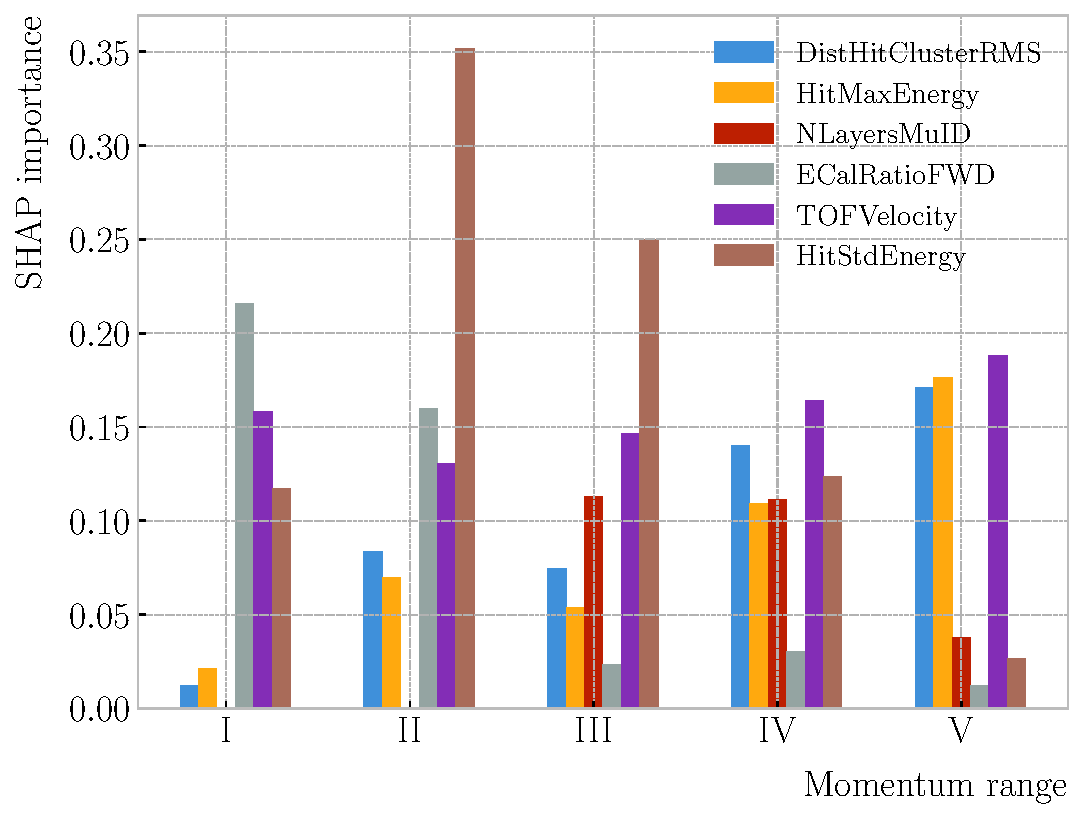
\includegraphics[width=.85\linewidth]{Images/GArSoft_PID/BDT/summary_top_six.pdf}
	\caption{Evolution of the SHAP importance for the top six most important features across all five momentum ranges.}
	\label{fig:bdt_shap_regions}
\end{figure}

The concept of Shapley values originated in the context of game theory, and it measures the marginal contribution of a feature in enhancing the accuracy of a classifier. Take $F$ to be the set of all features in a problem, and $S \subseteq F$ the subset of features. To compute the Shapley value of the $i$-th feature, one has to train a model with that feature present, $f_{S \cup \{i\}}$, and another model trained without it, $f_{S}$. This has to be repeated for all possible combinations of subsets $S \subset F \setminus \{i\}$, and evaluating the models predictions on the appropriate sets of data $x_{S}$. This way, the Shapley value results:
\begin{equation}
	\varphi_{i} = \sum_{S \subset F \setminus \{i\}} \frac{|S|!(|F|-|S|-1)!}{|F|!} \left[f_{S \cup \{i\}}(x_{S \cup \{i\}}) - f_{S}(x_{S})\right].
\end{equation}

I trained the \texttt{GradientBoostingClassifier} from \texttt{scikit-learn} with the default configuration in order to evaluate both the Gini and Shapley importances. The Gini scores are automatically computed by \texttt{scikit-learn}, using the training data. For the Shapley importance, I used the implementation from the \texttt{SHAP} package, computing it using the test sample. The results can be seen in Fig. \ref{fig:bdt_pca_importance_ii} (right panel) and Fig. \ref{fig:bdt_pca_importance_iii} (right panel), again for the momentum ranges $0.3 \leq p < 0.8 ~ \mathrm{GeV}/c$ and $0.8 \leq p < 1.5 ~ \mathrm{GeV}/c$. The length of the bars denote either the SHAP (blue) or the Gini (red) importance of the feature. One interesting thing to notice is that, when looking at the Gini importance, there is always one feature that dominates over the rest. This is not the case for the SHAP importance, where importances tend to be more balanced.

\begin{figure}[p]
	\centering
	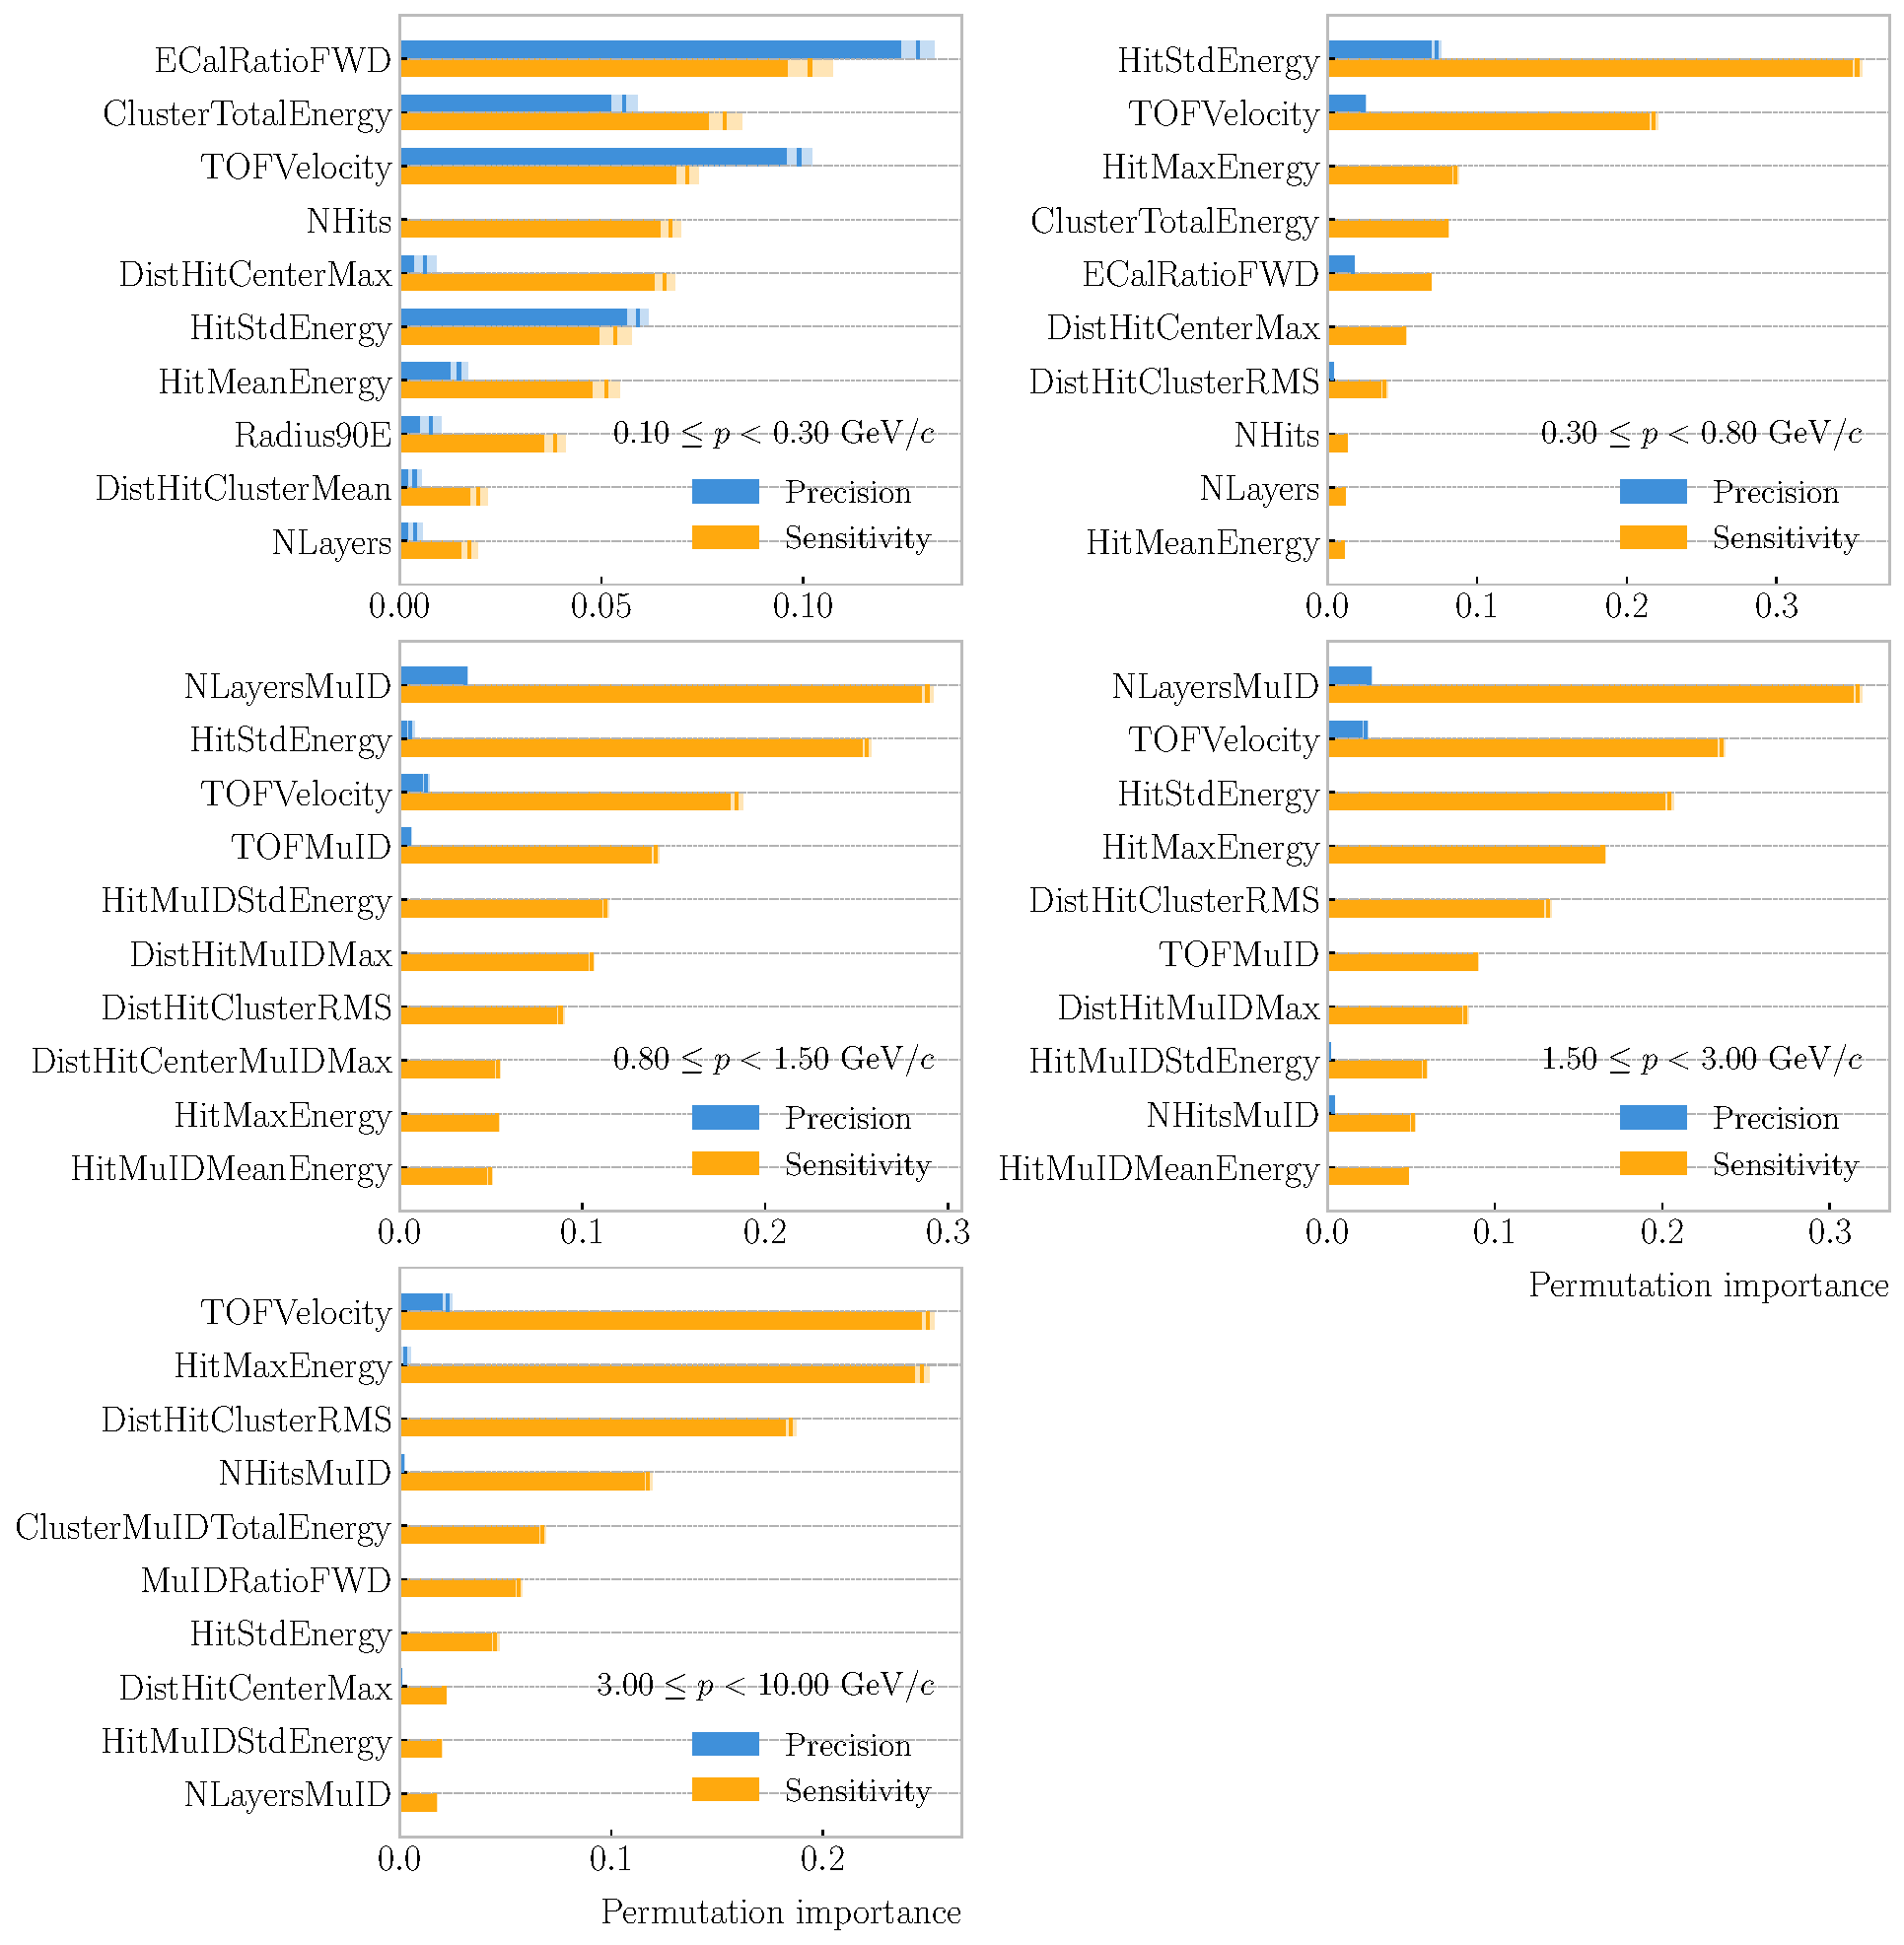
\includegraphics[width=.99\linewidth]{Images/GArSoft_PID/BDT/summary_permutation.pdf}
	\caption{Permutation importances for the ten most important features in the different momentum ranges (from left to right, top to bottom, in increasing momentum order). The bars indicate the effect that permutations of each feature have on the purity (blue) and the sensitivity (yellow), the translucent regions representing one standard deviation around the central value.}
	\label{fig:bdt_permutations}
\end{figure}

Across all momentum ranges, I observe that the most important features are. For the five momentum ranges considered, only six variables sit in the top five at least once. Figure \ref{fig:bdt_shap_regions} shows the evolution of the SHAP importance of these six features. It is interesting to see that the time-of-flight variable keeps its importance almost unchanged for all momenta. Also, it looks like the ECal energy ratio gets less relevant the higher the momentum is, but the RMS of the hit-to-cluster distance distribution and the maximum ECal hit energy become more important in the last momentum ranges.

The last step in the feature selection analysis is the feature permutation. This technique measures the contribution of each feature to the performance of a model by randomly shuffling its values and checking how some scores degrade. For the present case, I am interested in the precision or purity, and the sensitivity or efficiency, as these two are the most relevant metrics from a physics point of view. The \texttt{scikit-learn} module provides the user with a method to perform the permutation scans.

The results of these are shown in Fig. \ref{fig:bdt_permutations}. For the different momentum ranges I show the permutation importances for the ten most important features. For each of the variables I report the effect the permutations have on the precision (blue) and sensitivity (yellow) of the models. The bars indicate the importance value, with the lighter part representing one standard deviation around the mean (hinted as an additional vertical line). Something to notice is that, in the first momentum region, the feature permutations have an effect on both the precision and the sensitivity. However, for the rest the precision is almost unaffected, while the sensitivity changes are considerably larger.

It is also interesting to see that most of the variables identified as important here are the same I found when looking at the Shapley values. The behaviour of these across the momentum ranges is also similar, with the same patterns of some features being important at low momenta and then dropping in importance for the high momentum ranges.

Wit this, I conclude the study of the features. I have prepared the training and testing datasets and understood what features are likely to have the largest impact on the performance of the classifiers.

\subsection{Hyperparameter optimisation}

Any BDT requires the user to specify a number of parameters that will dictate its behaviour. They can be divided into two categories: (i) tree-specific parameters, which affect each individual tree in the model, and (ii) boosting parameters, which control the boosting operation in the model. The value of these so-called hyperparameters affect the performance and predictive power of the models. Therefore, one needs to carefully select their optimal values in order to extract as much information as possible from the data.

From all the parameters used to define a tree in the \texttt{scikit-learn} implementation of the BDT classifier, I only consider a subset of them. This is due to the fact that some are mutually exclusive, but also because I noticed that others have little effect on the problem at hand. Therefore, the parameters I investigate are the following:
\begin{itemize}
	\item \texttt{min_samples_split}: defines the minimum number of samples required in a node to be considered for splitting. Higher values prevent a model from learning relations which might be highly specific to the particular sample, but may led to under-fitting if the value is too low.
	\item \texttt{min_samples_leaf}: defines the minimum samples required in a leaf node. For imbalanced problems it should take a low value, as there will not be many cases where the minority class dominates.
	\item \texttt{max_depth}: maximum depth of a tree. Useful to prevent over-fitting, as higher depth will allow a model to learn relations specific to the training sample.
\end{itemize}
In the case of the boosting parameters, the ones I look at are:
\begin{itemize}
	\item \texttt{learning_rate}: determines the impact of each tree on the final outcome. Low values make the model robust to the specific characteristics of a tree, and thus allow it to generalise well. However, that usually requires a large number of trees to model the data properly.
	\item \texttt{n_estimators}: number of sequential trees to be trained. In general, BDTs are fairly robust at higher number of trees but it can still overfit at a point.
	\item \texttt{subsample}: fraction of observations to be selected for each tree. Values slightly less than $1$ make the model robust by reducing the variance.
\end{itemize}

In general, hyperparameters depend on each other. Thus, it is not possible to optimise them independently. In the literature, we find two main strategies to explore the hyperparameter space. We could use a grid search, in which one discretises a portion of the space of hyperparameters and evaluates the model at each point. Another approach is the randomised search, where a certain number of random configurations of hyperparameters are explored.

In this case, I used the random search to scan the hyperparameter space. Also, because it is not guaranteed that a set of hyperparameters can be efficiently applied across different datasets, I perform the optimisation for each of the momentum ranges considered. Table \ref{tab:bdt_hyperpars} shows the list of hyperparameters considered, and the range within which I let them vary. I decided to fix the number of estimators to $400$ in all cases, as its value is correlated with that of the learning rate.

\begin{figure}[t]
	\begin{subfigure}{0.32\textwidth}
		\centering
		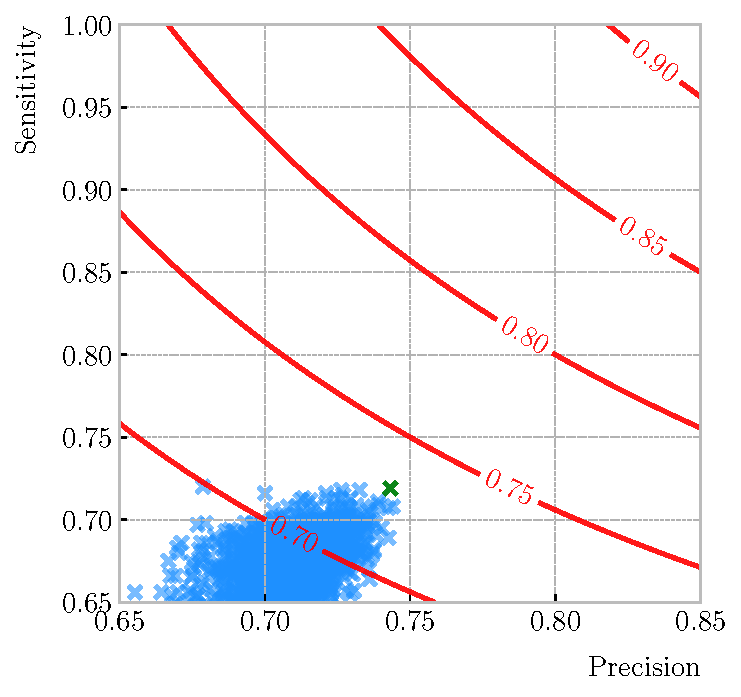
\includegraphics[width=.99\linewidth]{Images/GArSoft_PID/BDT/precision_vs_sensitivity_p0_0.20_sigmap_0.10.pdf}
	\end{subfigure}
	\begin{subfigure}{0.32\textwidth}
		\centering
		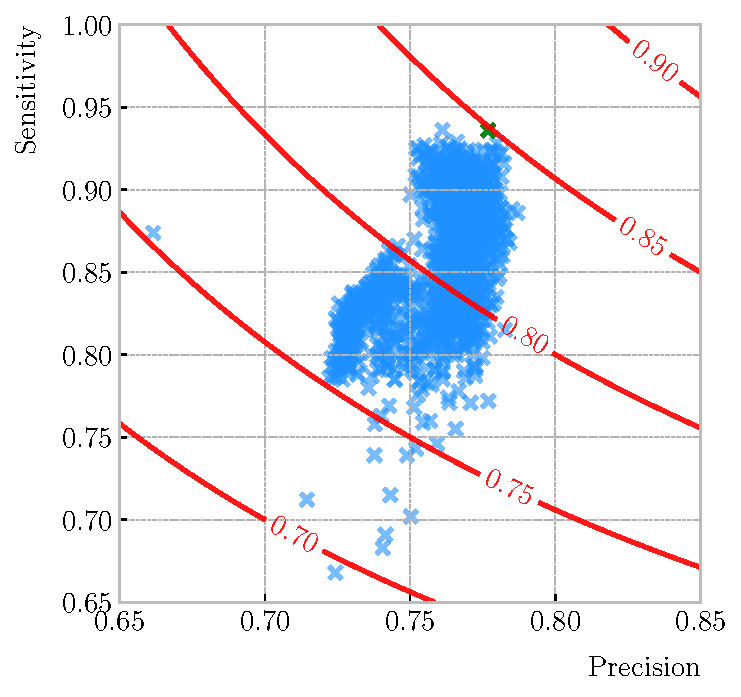
\includegraphics[width=.99\linewidth]{Images/GArSoft_PID/BDT/precision_vs_sensitivity_p0_1.15_sigmap_0.35.pdf}
	\end{subfigure}
	\begin{subfigure}{0.32\textwidth}
		\centering
		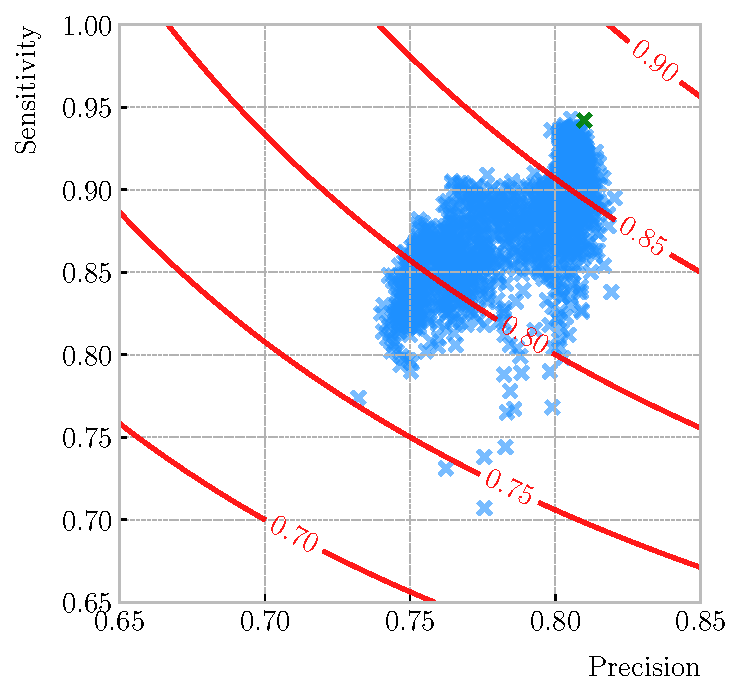
\includegraphics[width=.99\linewidth]{Images/GArSoft_PID/BDT/precision_vs_sensitivity_p0_6.50_sigmap_3.50.pdf}
	\end{subfigure}
	\caption[Values of the precision and sensitivity obtained for 10000 BDT hyperparameter configurations, for the momentum regions I, III and V.]{Values of the precision and sensitivity obtained for 10000 BDT hyperparameter configurations, for the momentum regions I, III and V. The red contours indicate the curves of equal $F_{1}$-score, while the green crosses are the selected configurations.}
	\label{fig:hyper_precision_sensitivity}
\end{figure}

I evaluate 10000 different hyperparameter configurations for each momentum range. For the hyperparameter tunning, I used subsamples containing $10\%$ of the full datasets, keeping the original proportions between classes, in order to reduce the computational load. The performance of the models was assessed using a stratified 3-fold cross-validation with replacement. Cross-validation involves dividing the data in a number of subsets, training the model using some of them, and testing it with the rest. In our case, I divide the data in 3 equal-sized subsets, maintaining the class proportions of the original dataset. Then, for 3 consecutive iterations, I train the models using 2 of the subsets while I compute the precision and sensitivity scores with the other. This approach provides a more robust estimate of the performance on unseen data.

\begin{table}[t]
	\caption{Optimal values of the hyperparameters used by the BDT, for each momentum range.}
	\begin{center}
		\begin{small}
			\begin{tabular}{l|l|lllll}
				\multirow{2}{*}{Hyperparameter} & \multirow{2}{*}{Range} & \multicolumn{5}{l}{Best value}                           \\[1mm] \cline{3-7}
												&                        & \rule{0pt}{1.1\normalbaselineskip}I & II & III & IV & V \\[1mm]
												\hline
				\rule{0pt}{1.1\normalbaselineskip}\texttt{min_samples_split}      & $[0.001, ~1]$          & 0.10     & 0.06      & 0.05       & 0.27      & 0.06     \\[2mm]
				\texttt{min_samples_leaf}       & $[0.001, ~1]$          & 0.02     & 0.03      & 0.01       & 0.02      & 0.07     \\[2mm]
				\texttt{max_depth}              & $\{2, ~3, ~..., ~8\}$  & 8        & 2         & 4          & 2         & 7      \\[2mm]
				\texttt{learning_rate}          & $[0.05, ~1]$           & 0.10     & 0.23      & 0.07       & 0.13      & 0.09     \\[2mm]
				\texttt{subsample}              & $[0.01, ~1]$           & 0.75     & 0.65      & 0.79       & 0.86      & 0.95    
			\end{tabular}
		\end{small}
	\end{center}
	\label{tab:bdt_hyperpars}
\end{table}

Figure \ref{fig:hyper_precision_sensitivity} shows the results in the precision versus sensitivity plane, for the momentum regions I, III and V (from left to right). The contours represent the curves of equal $F_{1}$-score, i.e. the harmonic mean of the precision and the sensitivity. In order to select the optimal configurations (indicated in the plots with a green cross), I chose the point with the highest $F_{1}$-score.

The results for the different momentum ranges are summarised in Tab. \ref{tab:bdt_hyperpars}. One can see some consistency in hyperparameter choices, with models generally preferring small values for the tree-specific parameters, small learning rate, and relatively large subsample sizes.

\begin{table}[t]
	\caption{Performance metrics of the BDTs with optimal hyperparameters, for the different momentum ranges.}
	\begin{center}
		\begin{small}
			\begin{tabular}{l|lllll}
				\multirow{2}{*}{Metric} & \multicolumn{5}{l}{Value $\pm ~ 1\sigma$}                                                                \\[2mm] \cline{2-6}
										& \rule{0pt}{1.1\normalbaselineskip}I                 & II                & III               & IV                & V                 \\[2mm] \hline
										\rule{0pt}{1.1\normalbaselineskip}Accuracy                & $0.779 \pm 0.003$ & $0.812 \pm 0.003$ & $0.846 \pm 0.002$ & $0.861 \pm 0.003$ & $0.874 \pm 0.002$ \\[2mm]
				Precision               & $0.769 \pm 0.003$ & $0.752 \pm 0.005$ & $0.788 \pm 0.002$ & $0.805 \pm 0.003$ & $0.815 \pm 0.003$ \\[2mm]
				Sensitivity             & $0.745 \pm 0.009$ & $0.921 \pm 0.006$ & $0.965 \pm 0.002$ & $0.967 \pm 0.002$ & $0.976 \pm 0.001$ \\[2mm]
				$F_{1}$-score           & $0.757 \pm 0.004$ & $0.828 \pm 0.003$ & $0.867 \pm 0.002$ & $0.879 \pm 0.002$ & $0.889 \pm 0.002$ \\[2mm]
				ROC AUC                 & $0.868 \pm 0.003$ & $0.865 \pm 0.003$ & $0.899 \pm 0.002$ & $0.902 \pm 0.002$ & $0.911 \pm 0.001$
			\end{tabular}
		\end{small}
	\end{center}
	\label{tab:bdt_metrics}
\end{table}

Now that I have obtained the optimal values of the hyperparameters, I can train the different BDTs. In this case I use the complete datasets, keeping $20\%$ of the data for testing. Table \ref{tab:bdt_metrics} shows the values of the different performance metrics obtained using the selected hyperparameters and 5-fold cross-validation. The last row indicates the value of the area under the receiver operating characteristic (ROC) curve. This represents the sensitivity of a model as a function of the false positive rate. I have included it here as it is a classic model metric used in the machine learning community. Overall, there is a clear trend of models performing better at higher momentum.

\subsection{Probability calibration}

So far, the trained BDTs are able to provide predictions of the class labels. Ideally, one would like the output of a classifier to give a confidence level about the prediction. However, it is not straightforward to interpret the outputs of our BDTs in terms of probabilities.

\begin{figure}[t]
	\centering
	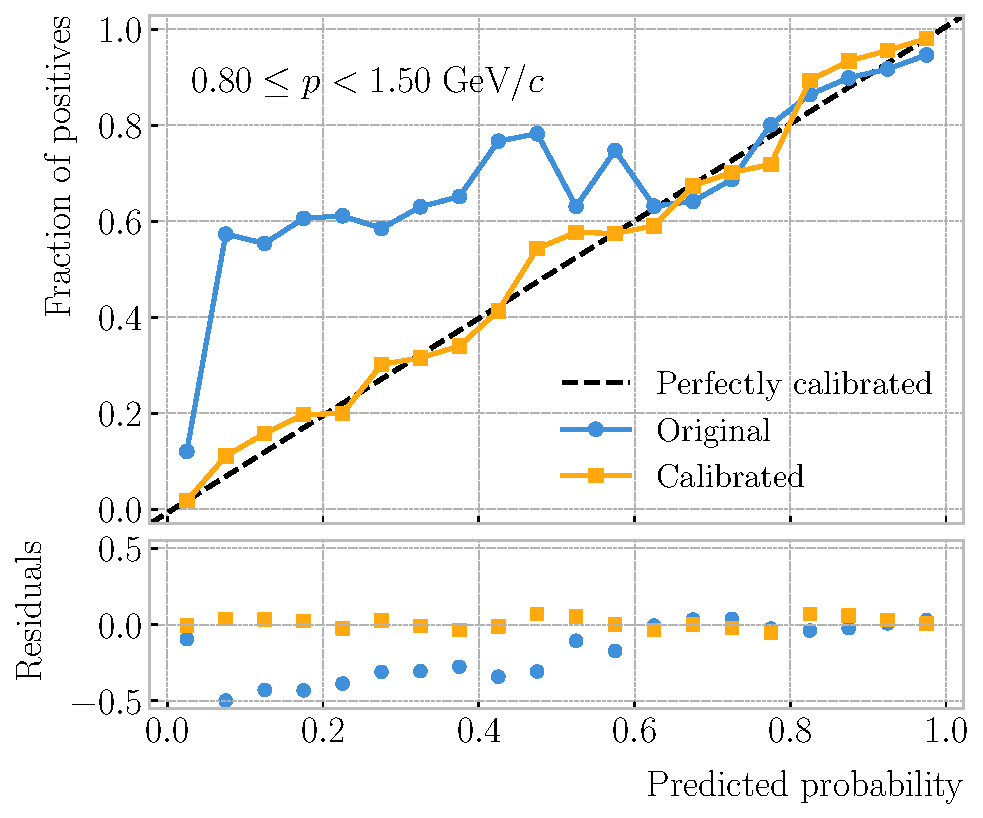
\includegraphics[width=.75\linewidth]{Images/GArSoft_PID/BDT/ecal_bdt_output_example_calibration_curves.pdf}
	\caption{Reliability diagrams for the BDT classifier used in the momentum range $0.3 \leq p < 0.8 ~ \mathrm{GeV}/c$, both for the original (blue circles) and calibrated (yellow squares) responses. For reference, the response of a perfectly calibrated classifier is also shown (black dashed line).}
	\label{fig:bdt_calibration_curves}
\end{figure}

A way to visualise how well the predictions of a classifier are calibrated is using reliability diagrams \cite{Wilks1995}. They represent the probability of the positive label versus the probability predicted by the classifier. These can be obtained by binning the predicted probabilities, and then compute the conditional probability $P(y_{true}=1|y_{i} \leq y_{pred} < y_{i+1})$ by checking the fraction of true positive instances in each bin. The reliability diagram of a perfectly calibrated classifier would be a diagonal line.

In this case, I try to correct the raw response of the classifiers by applying a sigmoid function:
\begin{equation}
	\sigma(x;~A,B) = \frac{1}{1+\mathrm{e}^{Ax+B}},
\end{equation}
where the parameters $A$ and $B$ are real numbers determined using the method of least squares.

\begin{figure}[t]
	\centering
	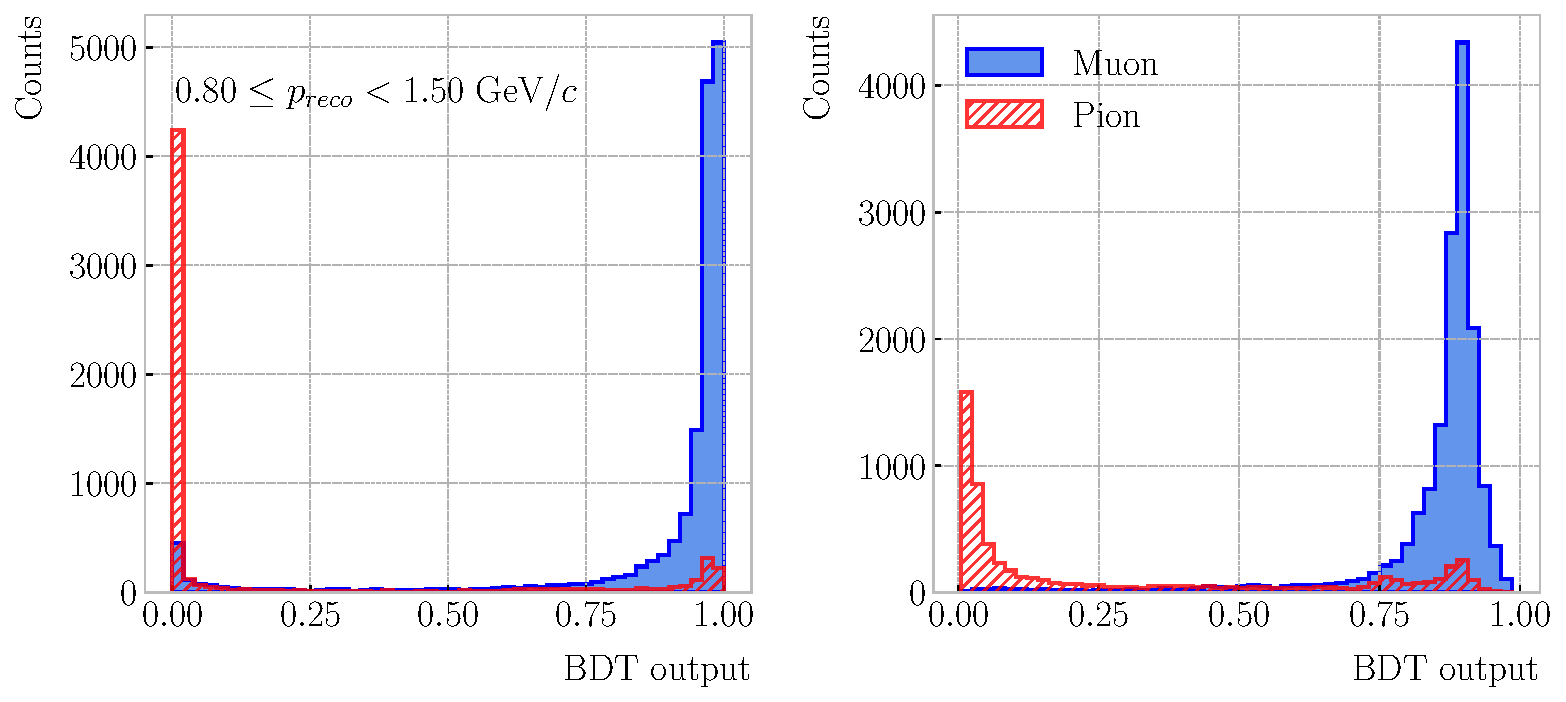
\includegraphics[width=.95\linewidth]{Images/GArSoft_PID/BDT/ecal_bdt_output_example_calibration.pdf}
	\caption{Uncalibrated (left panel) and calibrated (right panel) predicted probabilities assigned by the BDT classifiers for true muons (blue) and charged pions (red) in the momentum range $0.3 \leq p < 0.8 ~ \mathrm{GeV}/c$.}
	\label{fig:bdt_calibration_output}
\end{figure}

For each classifier, I perform a grid search to obtain the optimal values of $A$ and $B$. For any pair, I compute the predicted probabilities as $y_{pred} = \sigma(y_{raw};~A,B)$, where $y_{raw}$ are the raw predictions of the classifier\footnote{In \texttt{scikit-learn} these correspond to the outputs of the \texttt{decision_function} method.}. Then, I calculate the corresponding reliability curve, and take the sum of the squared residuals between it and the response of the perfectly calibrated classifier.

Figure \ref{fig:bdt_calibration_curves} shows the reliability diagrams for the original (blue) and calibrated (yellow) probability predictions of the classifier for the III momentum range, $0.3 \leq p < 0.8 ~ \mathrm{GeV}/c$. The original response of the classifier is given by $y_{pred} = \sigma(y_{raw};~-2,0)$, which is the transformation applied by \texttt{scikit-learn} to produce the probability estimate. Notice how the calibrated prediction matches the ideal response much better than the original, across all the probability range.

One can also compare the responses of the uncalibrated and calibrated classifiers broken down by true particle type, as shown in Fig. \ref{fig:bdt_calibration_output}. It can be seen that the distributions for both muons (blue) and charged pions (red) smoothen after calibration, but still the separating power of the classifier remains unchanged.

At this point, having the trained classifiers and the probability calibration parameters, I am able to assess the performance of the classification strategy in a physics-relevant case.

\subsection{Performance}

\section{ECal time-of-flight}\label{section:tof}

Looking at Fig. \ref{fig:dEdx_vs_momentum_regions}, it is clear that for momentum values in the range $1.0-3.0 ~ \mathrm{GeV}/c$ it is not possible to separate pions and protons using a $\left<\mathrm{d}E/\mathrm{d}x\right>$ measurement in the HPgTPC. However, in the previous section I assumed that protons at those energies could be identified by other means, and therefore were not an issue for the muon and pion discrimination.

Some detectors, like ALICE \cite{ALICE2011} or the ILD concept \cite{Einhaus2021}, complement the PID capabilities of their gaseous trackers with time-of-flight measurements. The use of fast timing silicon sensors, with hit time resolutions under $100~\mathrm{ps}$, would allow for the identification of charged hadrons via a ToF measurement up to $5.0 ~ \mathrm{GeV}/c$. In the case of ND-GAr, one could think of using the inner layers of the ECal, the ones consisting of high-granularity tiles, to obtain a ToF-based PID, with some inputs from the TPC.

Measuring the momentum and the velocity of a charged particle allows for a determination of the mass through the relativistic momentum formula:
\begin{equation}\label{8.19}
	m = \frac{p}{\beta} \sqrt{1-\beta^{2}}.
\end{equation}
In our case, the momentum is measured in the TPC, using the curvature and the dip angle of the helix inside the magnetic field. The velocity of the particle can be written as:
\begin{equation}
	\beta = \frac{\ell_{track}}{c \tau},
\end{equation}
where $\ell_{track}$ is the length of the track, and $\tau$ the arrival time to the ECal.

In GArSoft, the track length is computed at the Kalman filter stage. It is simply the sum of the line segments along the track, either in the forward or backward fit. In this case, because we are only interested in the particles that make it to the ECal, I choose the fit direction based on the results of the track-cluster associations.

\begin{figure}[t]
	\centering
	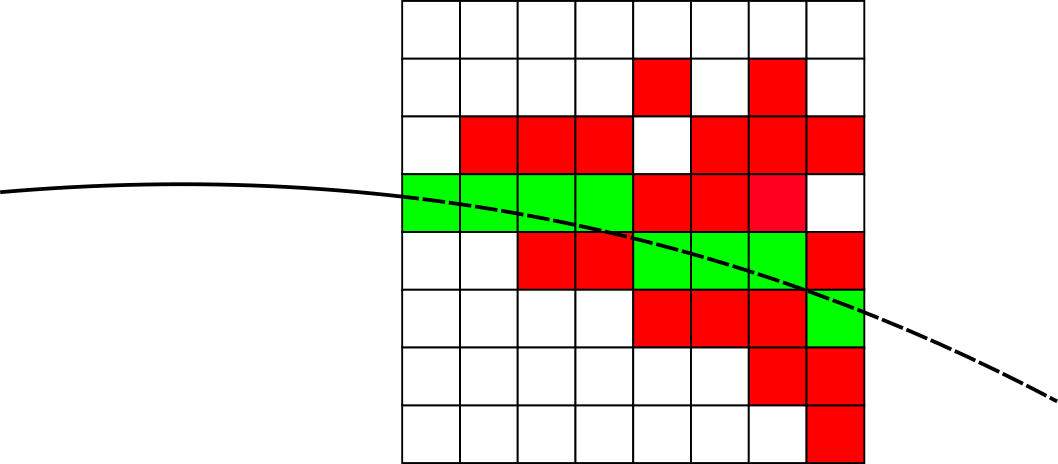
\includegraphics[width=.75\linewidth]{Images/GArSoft_PID/tof/tof_diagram.png}
	\caption{Schematic of the hit selection used for the ToF measurement. The grid represents the layers of the inner ECal, with coloured squares indicating the tiles with hits. Green squares indicate the selected hits.}
	\label{fig:tof_diagram}
\end{figure}

Additionally, because the last $30~\mathrm{cm}$ of the TPC radius are uninstrumented\footnote{Note to self: check this number.}, I need to correct for the length of the tracks. Using the track fit parameters to propagate the helix to its entry point in the ECal, one can write the total track length as:
\begin{equation}
	\ell_{track} = \ell + \left| \frac{\phi_{\mathrm{EP}} - \phi}{R^{-1}} \right| \sqrt{1+\mathrm{tan}^{2}\lambda},
\end{equation}
where $\phi_{\mathrm{EP}}$ is the angle of rotation at the entry point to the calorimeter, and $\ell$, $\phi$, $R$ and $\lambda$ are the track length, angle of rotation, radius of curvature and dip angle at the last point in the fit, respectively.

To test the idea of performing a ToF measurement with the inner ECal, I generated two data samples. Each consists of 10000 single particle events, either charged pions or protons. Their momenta are uniformly distributed in the range $0.5-5.0~\mathrm{GeV}/c$, and their directions are isotropic. I process each sample using different values of the time resolution, from $\Delta \tau = 0$, the perfect time resolution case for comparison, to the current nominal value of $\Delta \tau = 0.7~\mathrm{ns}$, and the worse scenario of $\Delta \tau = 1.0~\mathrm{ns}$.

\subsection{Arrival time estimations}

In the simulation, the limited time resolution of the ECal is taken into account by applying a Gaussian smearing to the true hit times. Other effects, like the digitisation of the signals, are not taken into account and fall beyond the scope of this study. After the track-cluster, one ends up with a collection of ECal hits associated to each particle. From these, the arrival time of the particle to the ECal can be extracted.

The simplest possibilities are to either take the time of the earliest hit or the hit closest to the entry point. Because these two coincide, in general, I focused only in the earliest hit time. However, this needs to be corrected, to account for the distance travelled from the entry point to the position of the hit:
\begin{equation}\label{8.22}
	\tau_{earliest} = \tau_{hit} - \frac{d_{\mathrm{EP}-hit}}{c},
\end{equation}
where $\tau_{hit}$ is the time of the earliest hit, and $d_{\mathrm{EP}-hit}$ is the distance between that hit and the entry point of the particle to the ECal. This is computed as the arc length between the entry point and the point of the extrapolated helix up to the layer of the hit. This way of correcting the time assumes $c$ for the propagation of the particle, which may lead to biased estimates.

\begin{figure}[t]
	\centering
	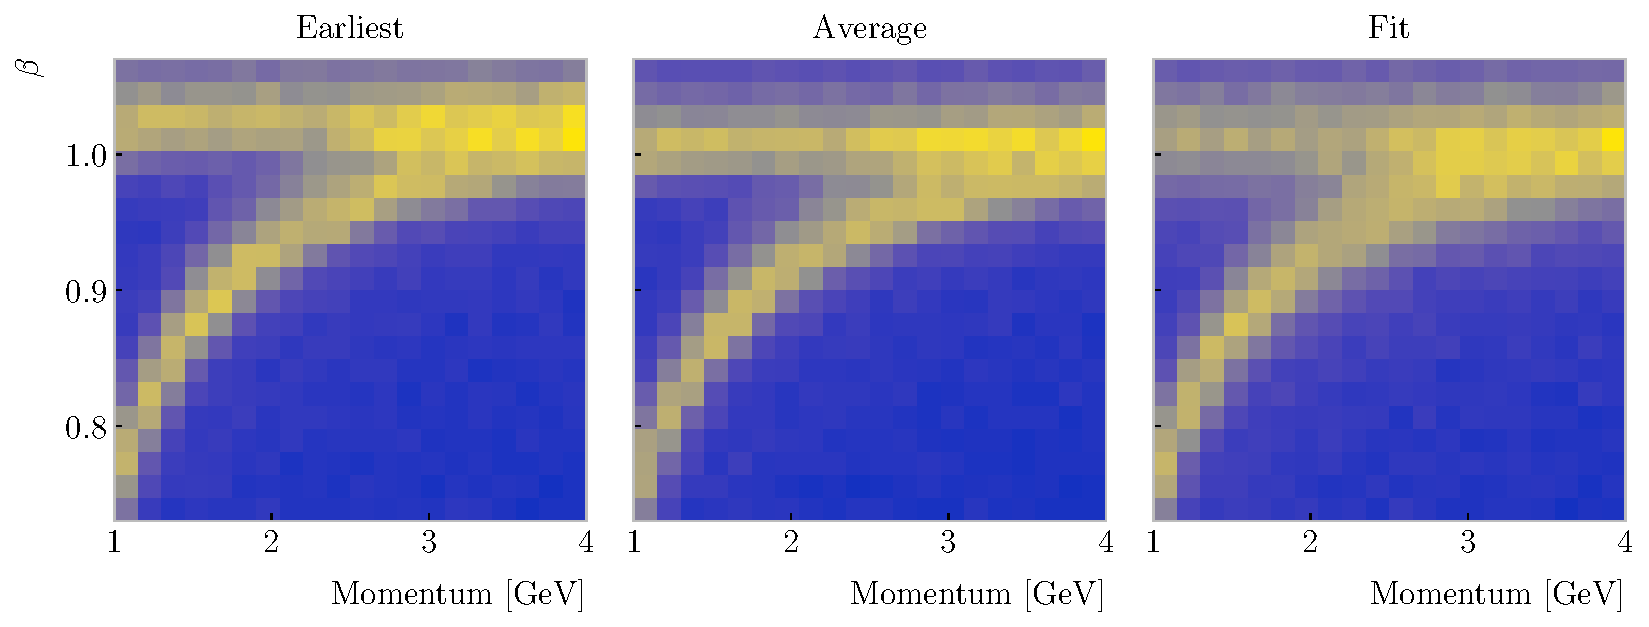
\includegraphics[width=.99\linewidth]{Images/GArSoft_PID/tof/beta_vs_momentum_comparison_delta_0.1.pdf}
	\caption{Particle velocity versus momentum measured with different ECal arrival time estimations. From left to right: earliest hit time, average hit time, and fitted hit time. In all cases the time resolution is $\Delta \tau = 0.1 ~ \mathrm{ns}$.}
	\label{fig:tof_beta_comp}
\end{figure}

I also tried to estimate the arrival times using information from the rest of the hits. In order to do this, as a simplifying assumption, I approximate the hadronic shower considering only its MIP component. For each layer, I keep only the hit in the tile closest to the point of the extrapolated track up to that layer. Figure \ref{fig:tof_diagram} shows an example of how this hit selection works. The dashed line represents the extrapolated track, while the coloured squares are the tiles containing hits. Green indicates the tiles closer to the track in each layer (in the sketch they correspond to the grid columns).

Now, I can use these collections of hits to estimate the arrival times. A possibility is to take the average of the times of the selected hits, denoted $\tau_{average}$. For that to work, one needs to correct these times, in a similar way as in Eq. (\ref{8.22}), before taking the average. However, as before, this correction assumes that the particle travels at the speed of light inside the ECal. Another option is to perform a linear fit to the hit times and the distances to the entry point. In that case, the arrival time would be the fitted value of the intercept, $\tau_{fit}$. This method would not assume a speed of light propagation.

Figure \ref{fig:tof_beta_comp} shows the velocity estimations as a function of the particle momentum, for the earliest hit time (left panel), average hit time (middle panel), and fitted hit time (right panel). The two bands correspond to the $\pi^{\pm}$ and the $p$ particles. $\Delta \tau = 0.1 ~ \mathrm{ns}$. Notice how, for the earliest hit time method, the velocities are significantly biased towards larger values. For the multi-hit methods, the $\tau_{fit}$ estimate appears to produce a larger variance than when using the $\tau_{average}$ method.

\subsection{Proton and pion separation}

Once we have the velocities of the particles, one can estimate their masses through Eq. (\ref{8.19}). The resulting mass spectra are shown in Fig. \ref{fig:tof_mass_spectra}. I computed the masses for the three arrival time estimates discussed above, and three different values of the time resolution: $\Delta \tau = 0.00$ (perfect time resolution), $\Delta \tau = 0.10 ~ \mathrm{ns}$, and $\Delta \tau = 0.70 ~ \mathrm{ns}$. Although in all cases we have the same number of events, it appears as if the entries in the histograms decrease as the time resolution increases. Sometimes, the particles get unphysical values of $\beta > 1$, and in turn they do not contribute to the mass spectra. This is more likely to happen for higher values of $\Delta \tau$.

\begin{figure}[t]
	\centering
	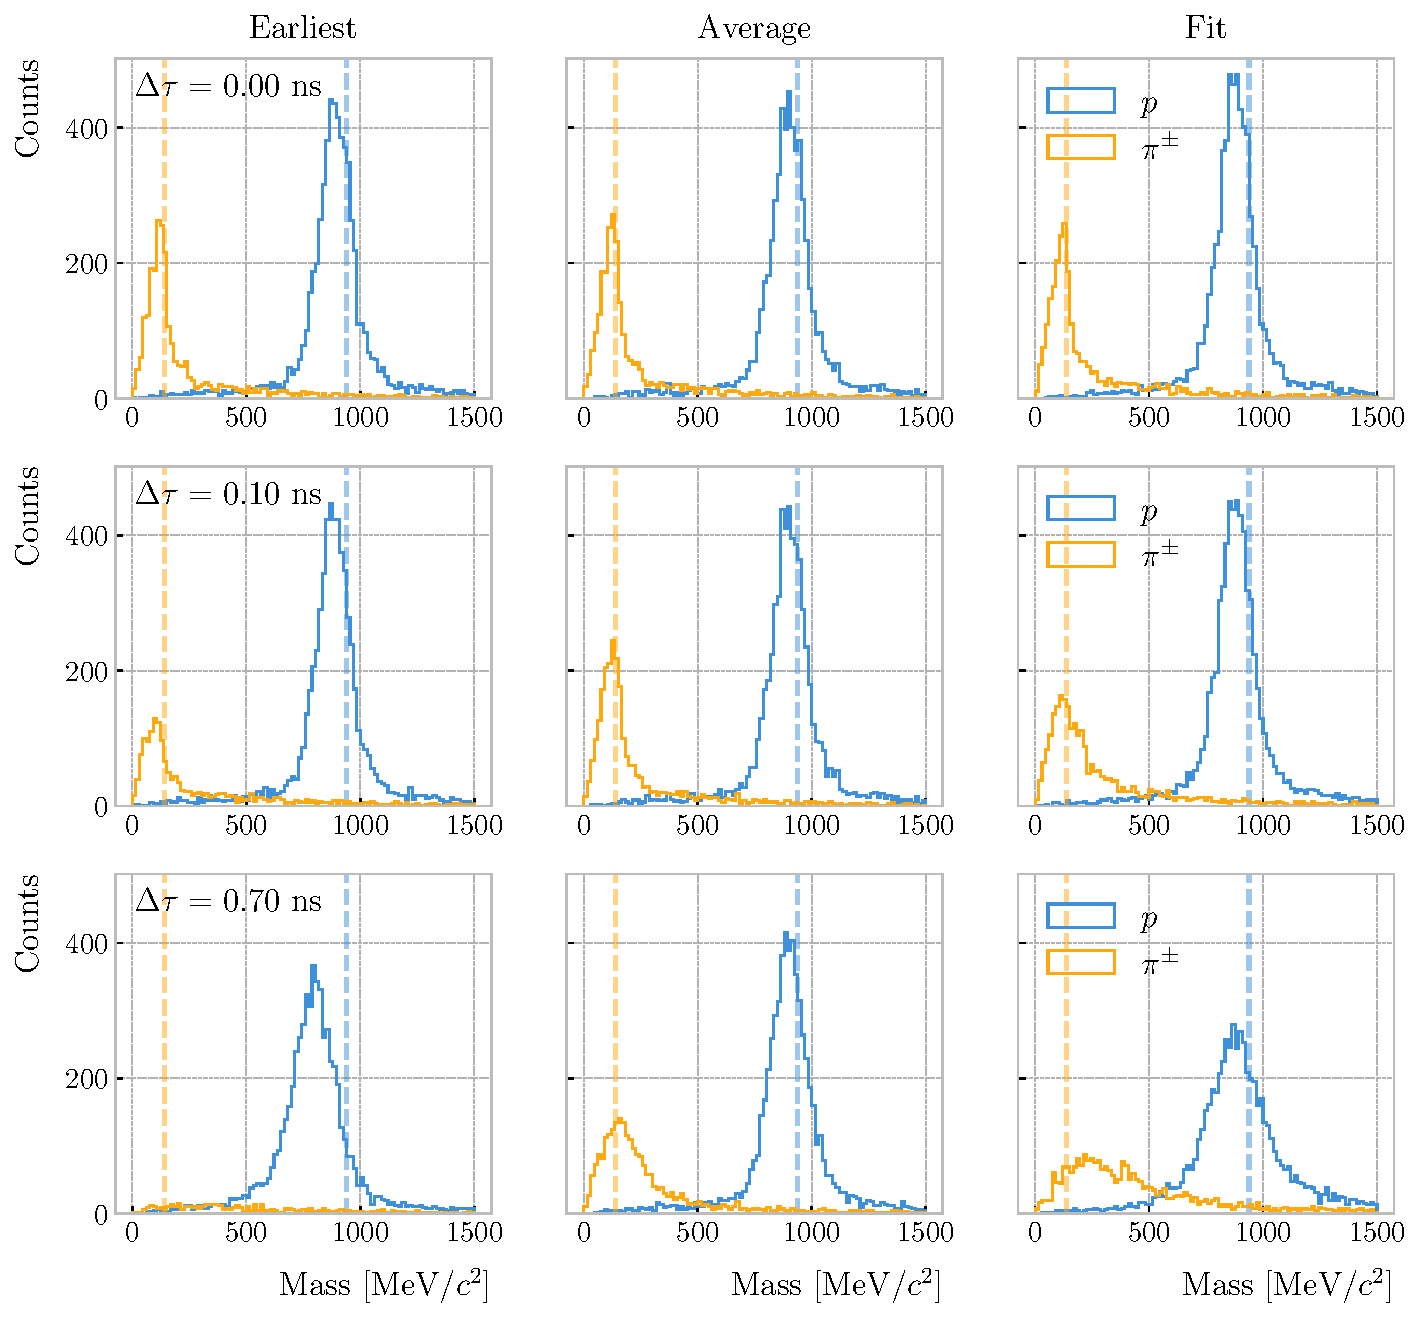
\includegraphics[width=.95\linewidth]{Images/GArSoft_PID/tof/reco_mass_comparison.pdf}
	\caption{Mass spectra for $p$ (blue) and $\pi^{\pm}$ (yellow) particles, using different ECal time resolution values (from top to bottom, in ascending order), and arrival time estimates. From left to right: earliest hit time, average hit time, and fitted hit time. The dashed lines indicate the true masses of the particles.}
	\label{fig:tof_mass_spectra}
\end{figure}

As noted before, the average hit time method produces the most robust estimates when increasing $\Delta \tau$. Intuitively this makes sense, as by taking the mean one averages out the effect of the Gaussian smearing. Going forward, I will use this arrival time estimator, as it appears to be the best performing one.

\begin{figure}[t]
	\centering
	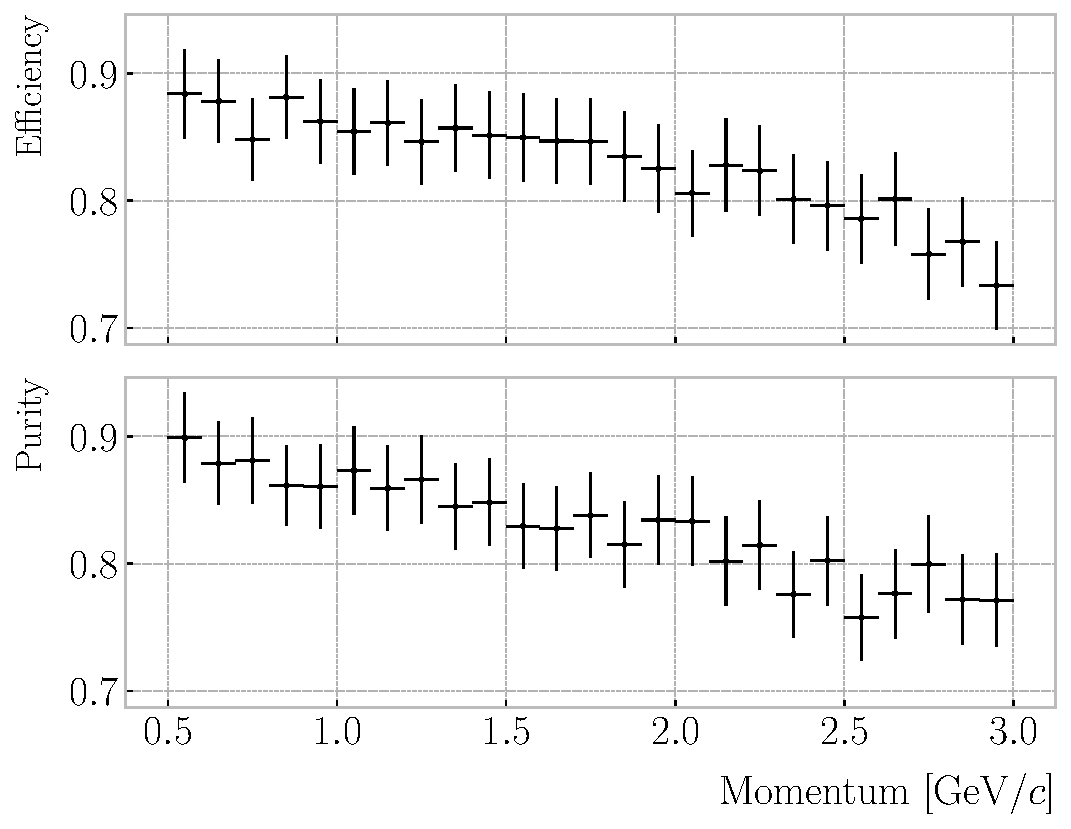
\includegraphics[width=.75\linewidth]{Images/GArSoft_PID/tof/proton_selection_beta_metrics.pdf}
	\caption{Efficiency (top panel) and purity (bottom panel) for the proton selection as a function of the momentum, for $\Delta \tau = 0.10 ~ \mathrm{ns}$.}
	\label{fig:tof_beta_selection}
\end{figure}

It is possible to use the velocity estimations to select a sample of protons. In this case, I do so by dividing the relevant momentum range in bins of $0.1~\mathrm{GeV}/c$. For each momentum bin, I compute the expected velocity for the protons via the inverse of Eq. (\ref{8.19}), and then take the fractional residuals of the measured velocities. Using that distribution, I choose the cut that maximises the $F_{1}$-score of the proton selection.

The results can be seen in Fig. \ref{fig:tof_beta_selection}, for the case $\Delta \tau = 0.10 ~ \mathrm{ns}$. As expected from Fig. \ref{fig:tof_beta_comp}, the performance of the selection degrades rapidly with increasing momentum. However, the purity is still around $75\%$ at $3.0~\mathrm{GeV}/c$. This is likely to be sufficient, as we do not expect protons or charged pions with higher energies from the beam neutrino interactions.

\begin{figure}[t]
	\centering
	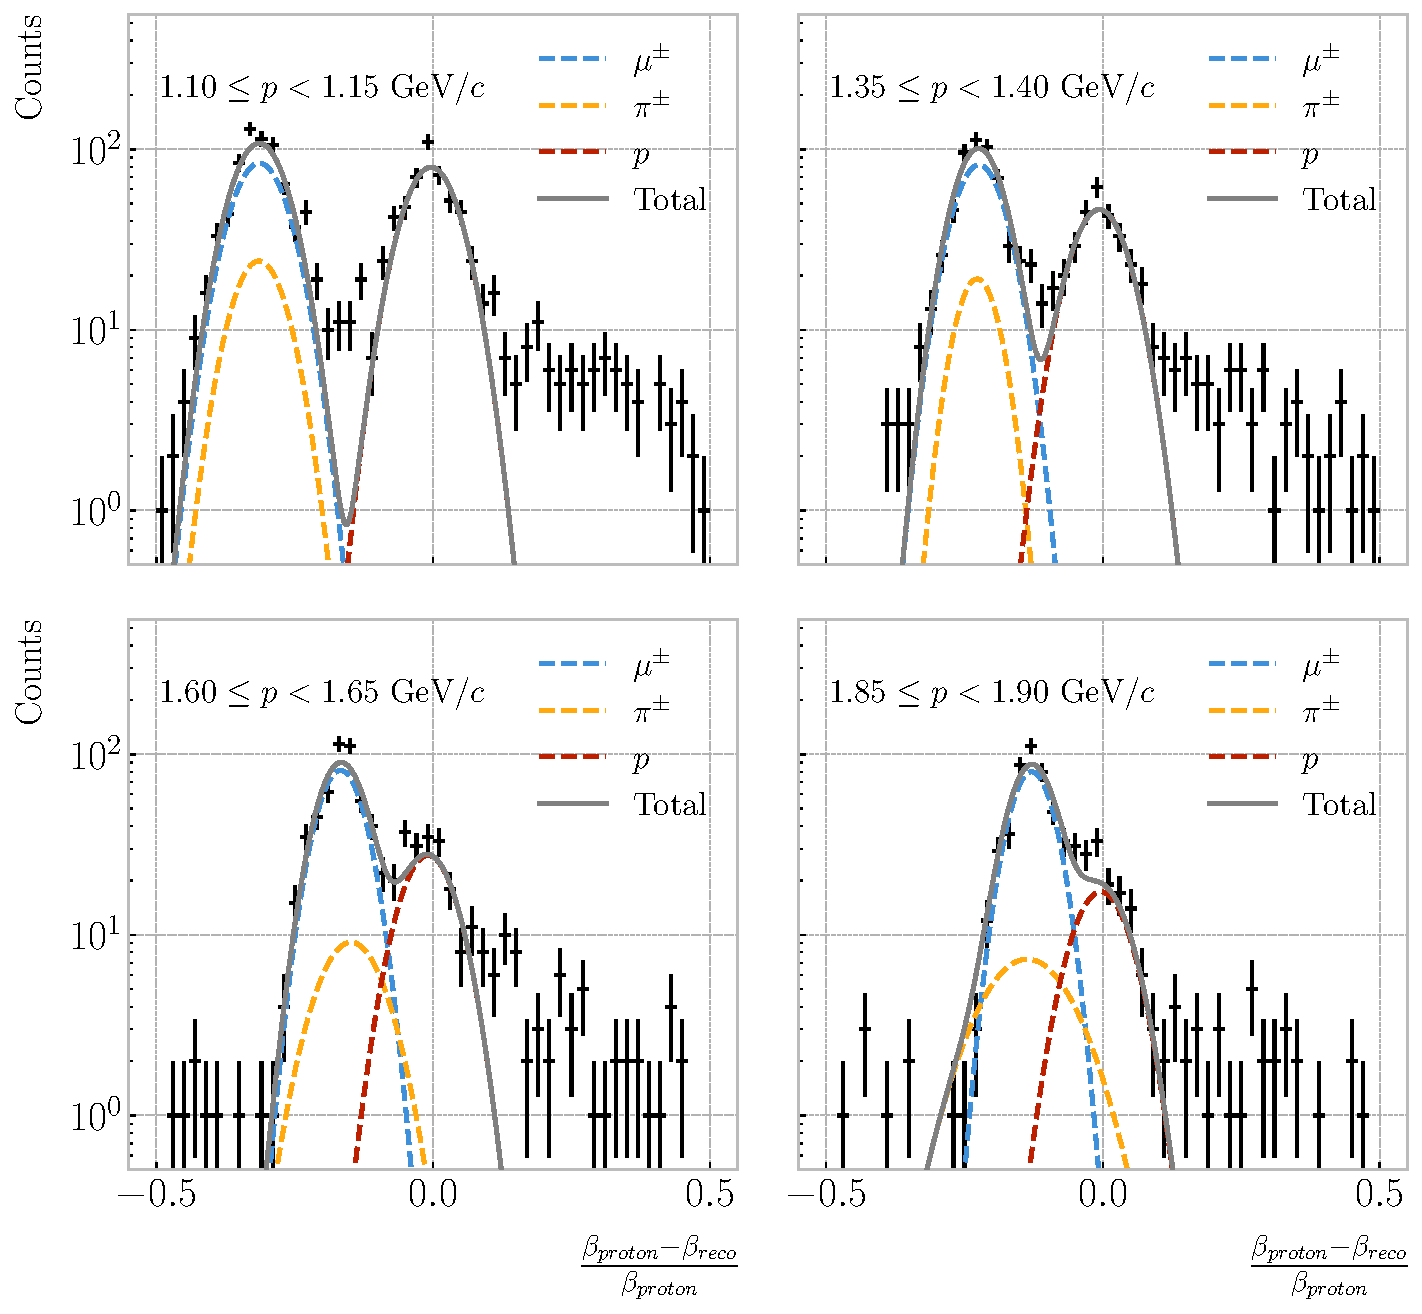
\includegraphics[width=.95\linewidth]{Images/GArSoft_PID/tof/numu_cc_proton_tof_summary.pdf}
	\caption{Distributions of the velocities measured by ToF with the
	inner ECal, for different momentum bins, in a FHC neutrino interaction sample. The Gaussian fits are performed around the maxima for each particle species.}
	\label{fig:tof_beta_fhc}
\end{figure}

Figure \ref{fig:tof_beta_fhc}

\section{Charged pion decay in flight}\label{section:pi_decay}

As discussed previously, in GArSoft the TPC tracks are formed after a pattern recognition algorithm and a Kalman filter are applied to the TPC clusters. These two steps can find discontinuities in the track candidates (e.g. due to a particle decay) when these so-called breakpoints are large enough. However, for some, more subtle, cases they may miss them and form a single reconstructed track. It has been noted in the literature that Kalman filters offer, as a by-product, additional information to form test statistics to identify these breakpoints \cite{Fruehwirth1988, Astier2000}.

\begin{figure}[t]
	\begin{subfigure}{0.5\textwidth}
		\centering
		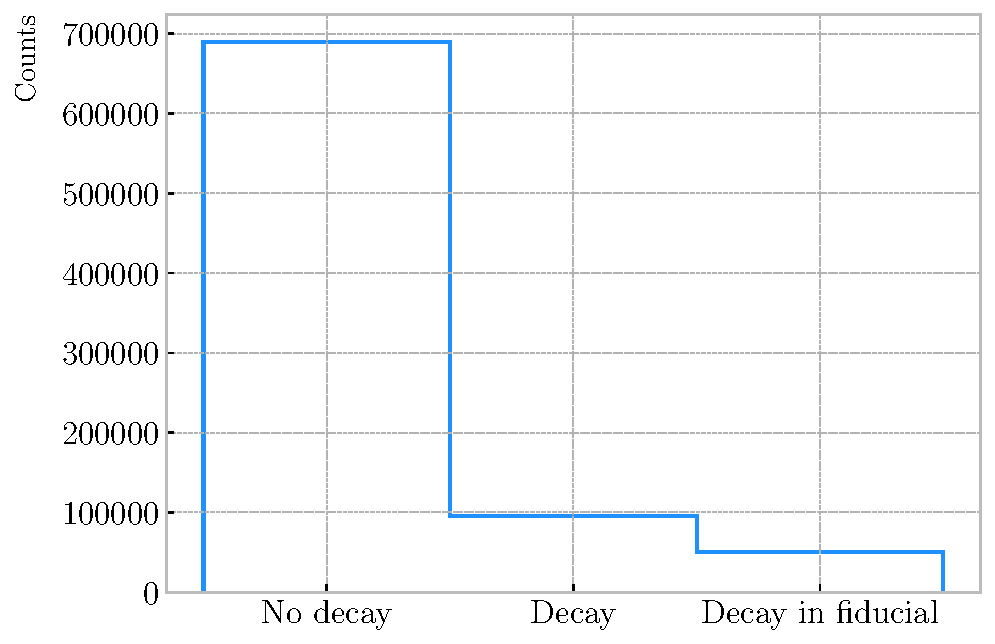
\includegraphics[width=.99\linewidth]{Images/GArSoft_PID/pion_decay/pion_decay_status.pdf}
	\end{subfigure}
	\begin{subfigure}{0.5\textwidth}
		\centering
		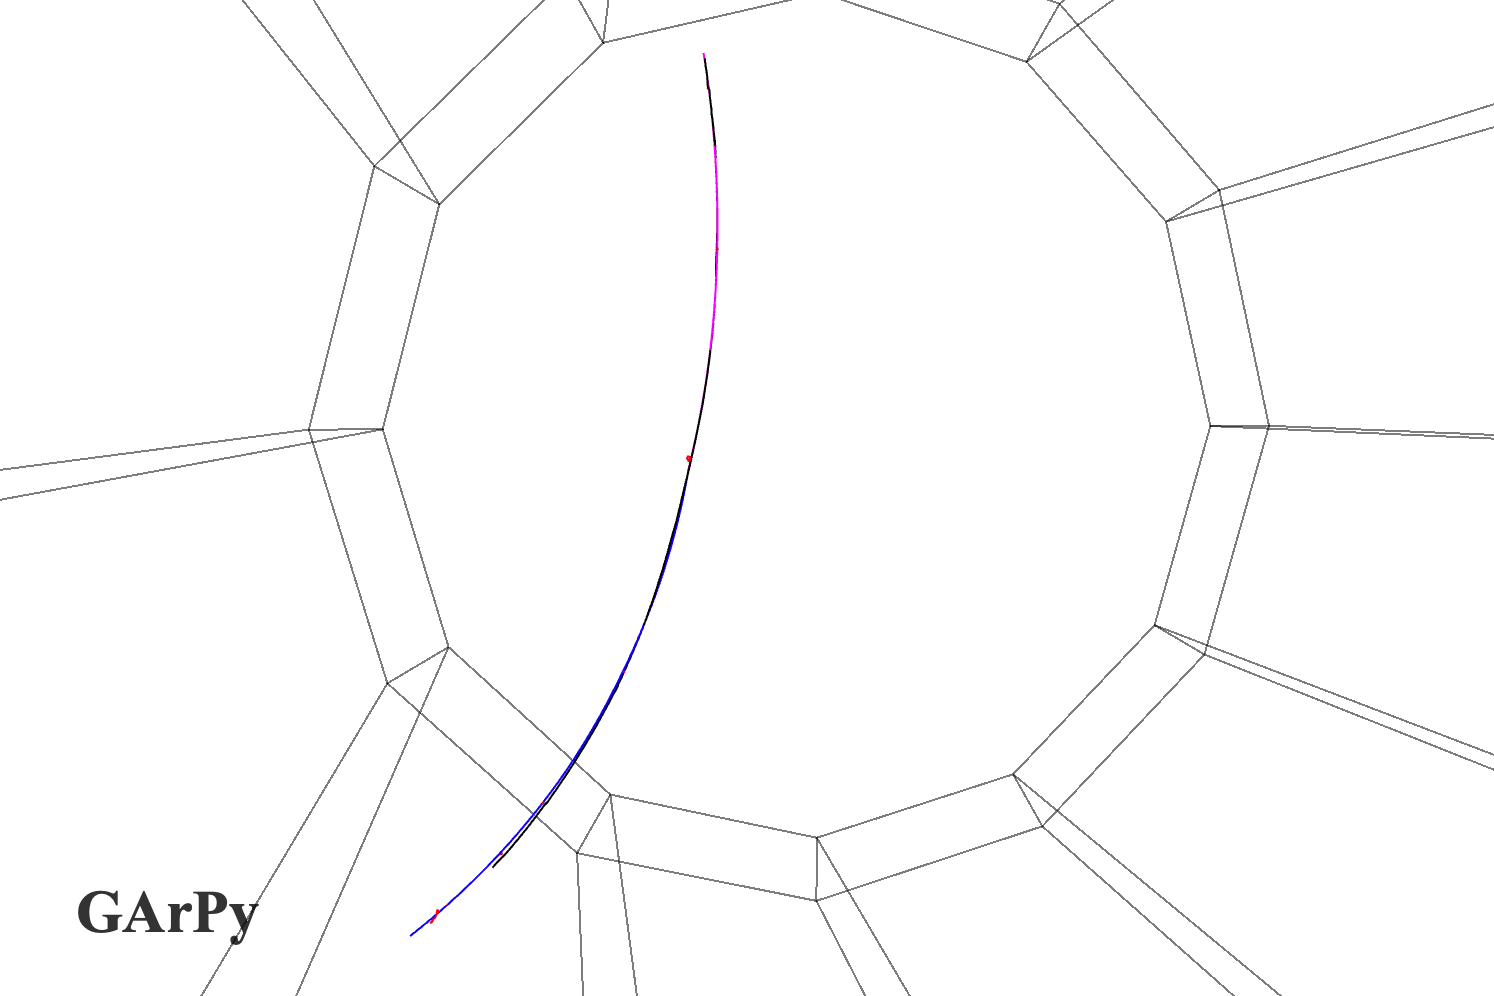
\includegraphics[width=.99\linewidth]{Images/GArSoft_PID/pion_decay/pion_decay_evd.png}
	\end{subfigure}
	\caption{Left panel: number of non-decaying, decaying and decaying in the fiducial volume pions for a MC sample of $100000$, $p=500 \ \mathrm{MeV}/c$ isotropic positively charged pions inside the TPC. Right panel: event display for a positive pion decaying inside the fiducial volume, with a single reconstructed track for the pion and muon system.}
	\label{fig:pion_decays}
\end{figure}

Considering the mean life of the charged pion, $\tau = (2.6033\pm0.0005)\times10^{-8} \ \mathrm{s}$, one can estimate that about $12\%$ of the pions with momentum $p \sim \mathcal{O}(500 \ \mathrm{MeV}/c)$ (roughly the peak of the pion momentum distribution in $\nu_{\mu}$ CC interactions off argon) decay inside the TPC. Figure \ref{fig:pion_decays} (left panel) shows the amount of charged pions decaying in the full TPC and fiducial volumes from an isotropic, monoenergetic sample of $100000$ negatively charged pions with $p=500 \ \mathrm{MeV}/c$. We see that about $10\%$ of those decayed, with more than half of them decaying inside the TPC fiducial volume.

Figure \ref{fig:pion_decays} (right panel) shows an example event display of a charged pion (magenta line) decays in flight inside the TPC, but because the angle of the muon (blue line) is small both were reconstructed as one single track (black line). In this case, the composite track reaches the ECal, where it undergoes a muon-like interaction, thus being classified as a muon.

A way to understand what decaying pion tracks were totally or partially reconstructed together with the daughter muon is looking at the relative energy contributions to the reconstructed track. In order to select a sample of such events, I require that a minimum $50\%$ of the total energy comes from the pion and at least $20\%$ from the muon.

\subsection{Track breakpoints}

To identify potential decays we can use the information we obtain from the Kalman filter at each step of the fitted track. The simplest test we can think about is computing the $\chi^{2}$ of the mismatch between all the parameters in the forward and the backward fits:
\begin{equation}
	\chi^{2 \ (FB)}_{k} = (\hat{\mathrm{x}}^{B}_{k}-\hat{\mathrm{x}}^{F}_{k})^{T}[V^{(\hat{\mathrm{x}}_{k},B)}+V^{(\hat{\mathrm{x}}_{k},F)}]^{-1}(\hat{\mathrm{x}}^{B}_{k}-\hat{\mathrm{x}}^{F}_{k}),
\end{equation}
where $\hat{\mathrm{x}}^{F}_{k}$, $\hat{\mathrm{x}}^{B}_{k}$ are the Kalman filter state vector estimates at step $k$ in the forward and backward fits and $V^{(\hat{\mathrm{x}}_{k},F)}$, $V^{(\hat{\mathrm{x}}_{k},B)}$ the covariance matrices of $\hat{\mathrm{x}}^{F}_{k}$ and $\hat{\mathrm{x}}^{B}_{k}$ respectively. Using the values of the $\chi^{2}$ at measurement $k$ for the forward and backward fits we can compute another $\chi^{2}$ value that characterises the overall track fit:
\begin{equation}
	\chi^{2}_{track} = \chi^{2 \ (F)}_{k} + \chi^{2 \ (B)}_{k} + \chi^{2 \ (FB)}_{k},
\end{equation}
which remains approximately constant for all $k$.

An alternative approach proposed in the context of the NOMAD experiment was using a fit with a more elaborate breakpoint hypothesis, so we can perform a comparison of the $\chi^{2}$ with and without breakpoints. This can be achieved by using some alternative parametrisation with extra parameters, which allows some of the track parameters to be discontinuous at certain points. A decay changes the momentum magnitude and direction, so we can use the new state vector:
\begin{equation}
	\alpha=\begin{pmatrix}y,& z,& 1/R_{F},& 1/R_{B},& \phi_{F},& \phi_{B},& \mathrm{tan}\lambda_{F},& \mathrm{tan}\lambda_{B}\end{pmatrix}^{T}.
\end{equation}

\begin{figure}[t]
	\centering
	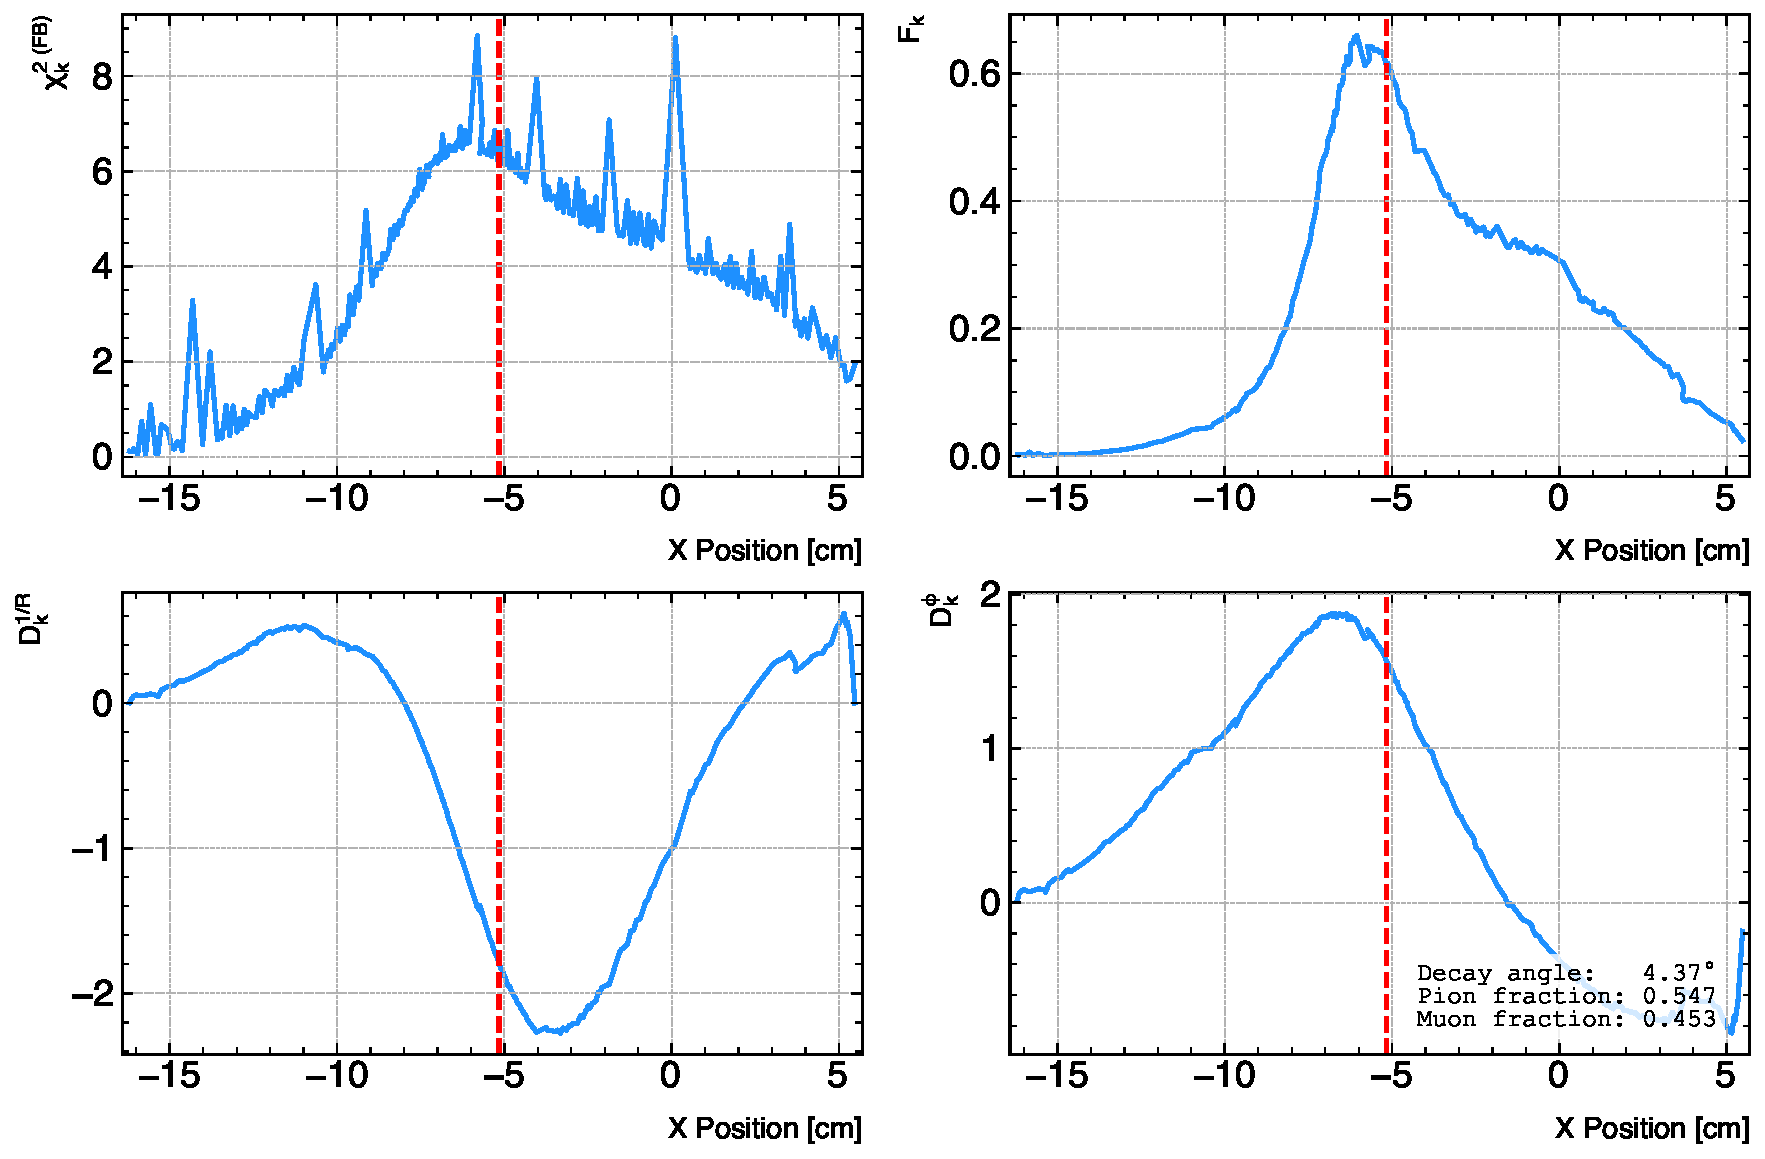
\includegraphics[width=.85\linewidth]{Images/GArSoft_PID/pion_decay/pion_decay_variables_event_425.pdf}
	\caption{Values of $\chi^{2 \ (FB)}_{k}$ (top left panel), $F_{k}$ (top right panel), $D^{1/R}_{k}$ (bottom left panel) and $D^{\phi}_{k}$ (bottom right panel) versus position along the drift direction for a reconstructed track in a positive pion decay event. The vertical red dashed line indicates the true location of the decay point.}
	\label{fig:breakpoint_variables_example}
\end{figure}

As we already have the estimates from the standard Kalman filter and their covariance matrices at each point, we do not need to repeat the Kalman fit for the new parametrisation. Instead, I can compute the values of $\alpha$ at each point $k$ that minimise the $\chi^{2}$ resulting from comparing them to $\{\hat{\mathrm{x}}^{B}_{k}, \hat{\mathrm{x}}^{F}_{k}\}$. Introducing the two $5 \times 8$ matrices:
\begin{equation}
	H^{F}=\begin{pmatrix}1&0&0&0&0&0&0&0 \\ 0&1&0&0&0&0&0&0 \\ 0&0&1&0&0&0&0&0 \\ 0&0&0&0&1&0&0&0 \\ 0&0&0&0&0&0&1&0\end{pmatrix}, \
	H^{B}=\begin{pmatrix}1&0&0&0&0&0&0&0 \\ 0&1&0&0&0&0&0&0 \\ 0&0&0&1&0&0&0&0 \\ 0&0&0&0&0&1&0&0 \\ 0&0&0&0&0&0&0&1\end{pmatrix},
\end{equation}
we can write this as:
\begin{equation}
	\begin{split}
		\chi_{k}^{2 \ (FB)} (\alpha) &= (\hat{\mathrm{x}}_{k}^{F}-H^{F}\alpha)^{T}\left[V^{(\hat{\mathrm{x}}_{k},F)}\right]^{-1}(\hat{\mathrm{x}}_{k}^{F}-H^{F}\alpha)\\
		&+(\hat{\mathrm{x}}_{k}^{B}-H^{B}\alpha)^{T}\left[V^{(\hat{\mathrm{x}}_{k},B)}\right]^{-1}(\hat{\mathrm{x}}_{k}^{B}-H^{B}\alpha).
	\end{split}
\end{equation}

The minimum of $\chi_{k}^{2 \ (FB)} (\alpha)$ is found when the measured new state vector takes the value:
\begin{equation}
	\hat{\alpha}_{k} = V^{(\hat{\alpha}_{k})} H^{T} (V^{(\hat{\mathrm{x}}_{k})})^{-1} \hat{\mathrm{X}},
\end{equation}
where $\hat{\mathrm{X}} = \{\hat{\mathrm{x}}^{B}_{k}, \hat{\mathrm{x}}^{F}_{k}\}$, $V^{(\hat{\mathrm{x}}_{k})}$ is the block diagonal matrix formed by $V^{(\hat{\mathrm{x}}_{k},F)}$ and $V^{(\hat{\mathrm{x}}_{k},B)}$ and $V^{(\hat{\alpha}_{k})}$ is the covariance matrix of $\hat{\alpha}_{k}$, given by:
\begin{equation}
	V^{(\hat{\alpha}_{k})} = \left(H^{T} (V^{(\hat{\mathrm{x}}_{k})})^{-1} H\right)^{-1}.
\end{equation}

\begin{figure}[t]
	\begin{subfigure}{0.5\textwidth}
		\centering
		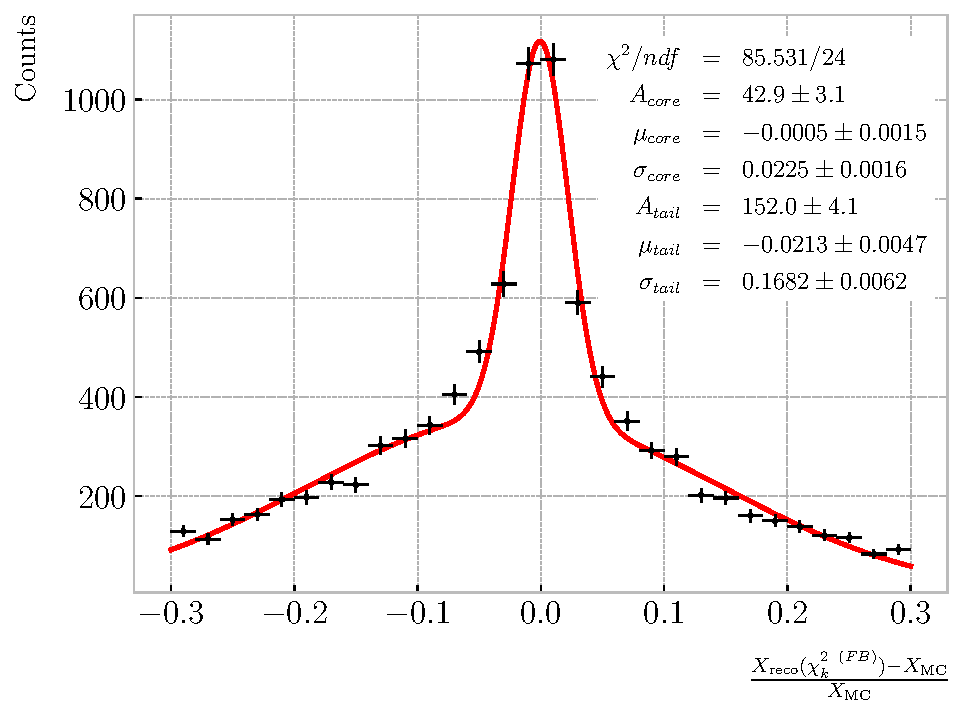
\includegraphics[width=.99\linewidth]{Images/GArSoft_PID/pion_decay/pion_decay_resolution_chisqfb.pdf}
	\end{subfigure}
	\begin{subfigure}{0.5\textwidth}
		\centering
		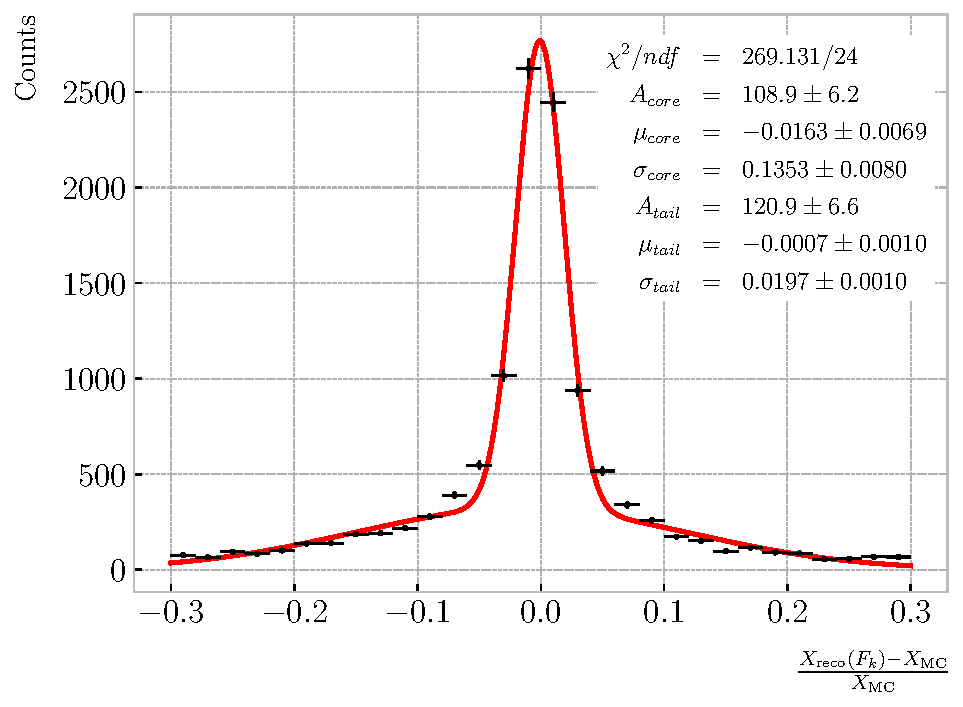
\includegraphics[width=.99\linewidth]{Images/GArSoft_PID/pion_decay/pion_decay_resolution_fisher.pdf}
	\end{subfigure}
	\caption{Fractional residual distributions of the true and reconstructed decay position along the drift coordinate, using the position of the maximum of $\chi^{2 \ (FB)}_{k}$ (left panel) and $F_{k}$ (right panel) as estimates of the decay position. Also shown are double Gaussian fits to these points (red lines).}
	\label{fig:pion_decay_resolution}
\end{figure}

From these new fit estimates we can compute the $F$ statistic, which tells us whether the model with breakpoint provides a statistically significant better fit:
\begin{equation}
	F_{k}=\left(\frac{\chi^{2}_{track,k}-\chi^{2}_{full,k}}{8-5}\right)/\left(\frac{\chi^{2}_{full,k}}{N-8}\right).
\end{equation}

One can also compute the signed difference of the duplicated variables divided by their standard deviation at each point. These represent how significant the discontinuity in each variable is. For any variable $\eta$ we can write it as:
\begin{equation}
	D^{\eta}_{k} = \frac{\hat{\eta}^{B}_{k}-\hat{\eta}^{F}_{k}}{\sqrt{\mathrm{Var}[\hat{\eta}^{F}_{k}]+\mathrm{Var}[\hat{\eta}^{B}_{k}]-2\mathrm{Cov}[\hat{\eta}^{F}_{k}, \hat{\eta}^{B}_{k}]}}.
\end{equation}
In our case, the relevant ones to look at are $D^{1/R}_{k}$ and $D^{\phi}_{k}$.

Figure \ref{fig:breakpoint_variables_example} shows the values of $\chi^{2 \ (FB)}_{k}$, $F_{k}$, $D^{1/R}_{k}$ and $D^{\phi}_{k}$ as functions of the position along the drift direction, for an example reconstructed track with $55.5\%$ of the energy coming from the charged pion and $45.5\%$ from the daughter muon. The true position of the decay is indicated (dashed red lines). Notice how $\chi^{2 \ (FB)}_{k}$ and $F_{k}$, $D^{1/R}_{k}$ reach their maxima near the decay point. In the former case this indicates a large forward-backward difference in the track fit. In the later it represents that the extended state vector improves the fit particularly around that point.

I can estimate the decay position finding resolution by computing the difference between the $X$ position of the maxima of $\chi^{2 \ (FB)}_{k}$ and $F_{k}$ and the $X$ position of the true decay. Figure \ref{fig:pion_decay_resolution} represent the  the fractional residual distributions for both cases, from the sample of tracks containing pion decays. Fitting a double Gaussian to the distributions (red lines) I find a resolution of $(3.31\pm0.15)\%$ and $(6.94\pm0.31)\%$ respectively.

In principle, the $F$-statistic should follow a Fisher distribution with $(8-5)$ and $(N-8)$ degrees of freedom under the null hypothesis. In most of our cases $N\sim\mathcal{O}(100)$, so the probability density functions will look very similar. In this case, it is safe to take the limit $N\rightarrow\infty$ in the Fisher PDF:
\begin{equation}
	\begin{split}
		\tilde{f}(x;a-b)&=\lim_{N \rightarrow \infty} f(x;a-b,N-a)\\
		&= \frac{2^{-\frac{a-b}{2}}}{\Gamma\left(\frac{a-b}{2}\right)}\left(a-b\right)^{\frac{a-b}{2}}x^{\frac{a-b}{2}-1}\mathrm{e}^{-\frac{a-b}{2}x}.
	\end{split}
\end{equation}
In our case $a-b = 8-5 = 3$, so we would obtain a p-value of $0.05$ at $x=2.60$.

\begin{figure}[t]
	\centering
	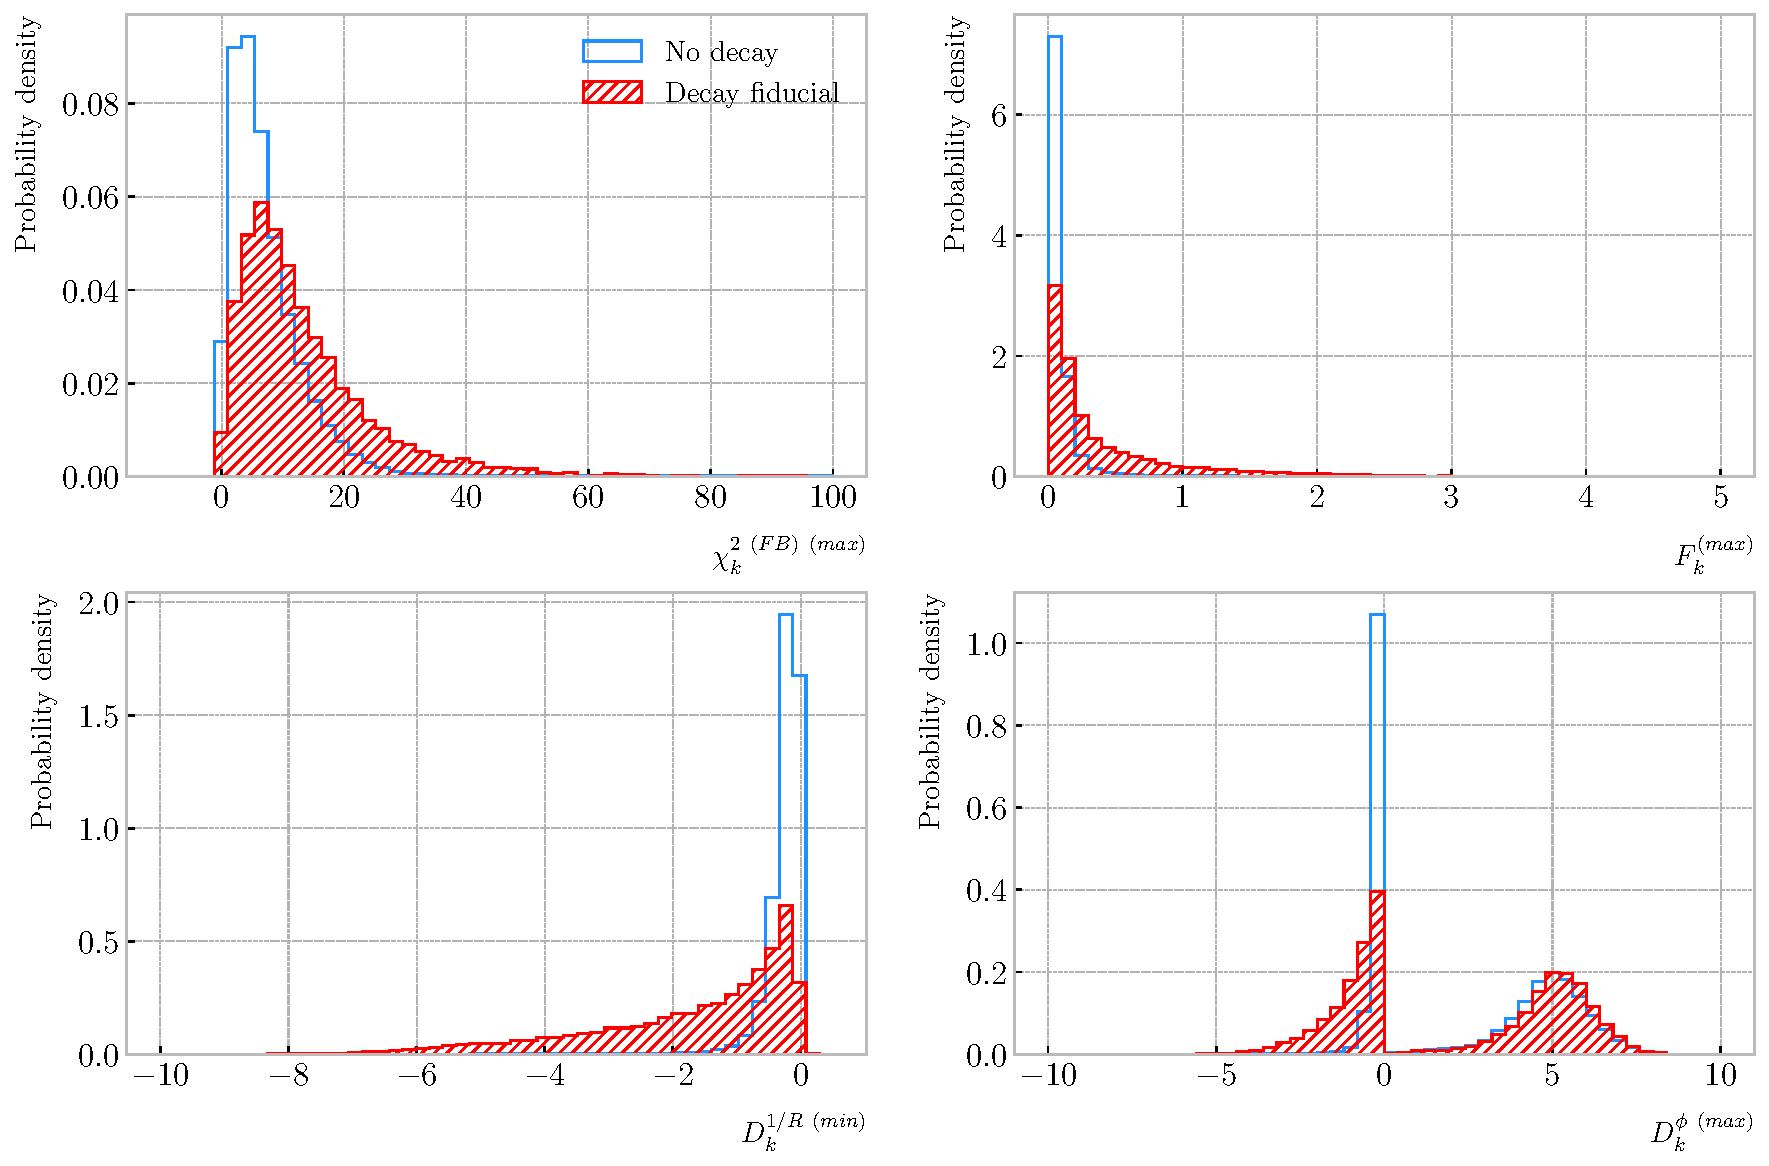
\includegraphics[width=.85\linewidth]{Images/GArSoft_PID/pion_decay/pion_decay_variables.pdf}
	\caption{Distributions of the extreme values of $\chi^{2 \ (FB)}_{k}$ (top left panel), $F_{k}$ (top right panel), $D^{1/R}_{k}$ (bottom left panel) and $D^{\phi}_{k}$ (bottom right panel) for non-decaying reconstructed pion tracks (blue) and tracks which include the decay inside the fiducial volume (red).}
	\label{fig:breakpoint_variables}
\end{figure}

Figure \ref{fig:breakpoint_variables} contains the distributions of the maxima of $\chi^{2 \ (FB)}_{k}$, $F_{k}$ and $D^{\phi}_{k}$ and the minima of $D^{1/R}_{k}$ for a sample of non-decaying pion tracks (blue) and another sample of reconstructed tracks containing part of the pion and the daughter muon from a decay inside the fiducial volume (red). Notice that, even though the values of $F^{(max)}_{k}$ for the decay sample are typically larger than for the non-decaying one, just a small fraction of the events go beyond the aforementioned value of $F=2.60$. Therefore, from a practical point of view, it is not the most efficient variable to use for selecting the decay events.

However, looking at the $D^{1/R \ (min)}_{k}$ distribution we can see there is a big difference between non-decaying and decaying events in this variable. One can use a combination of these four variables to distinguish between the pion decay events (signal) and the non-decaying pions (background).

\begin{figure}[t]
	\centering
	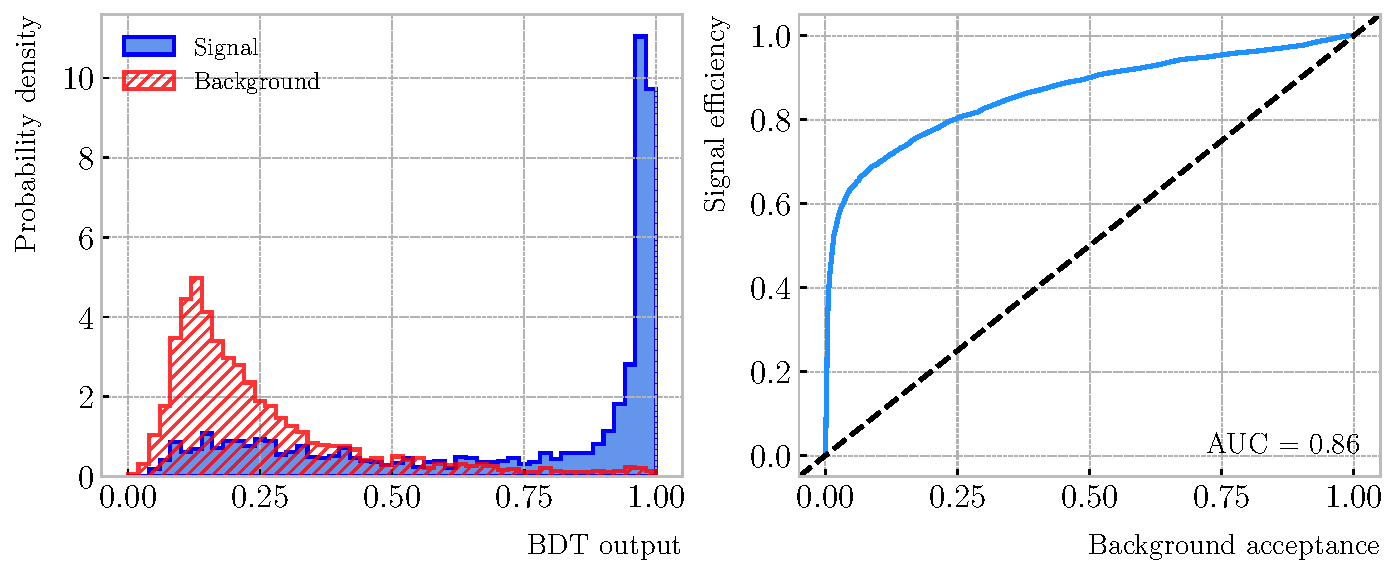
\includegraphics[width=.85\linewidth]{Images/GArSoft_PID/pion_decay/pion_decay_summary_bdt.pdf}
	\caption{Left panel: distributions of the predicted probabilities assigned by the BDT classifier to a test sample of decaying pion+muon tracks (blue) and non-decaying pion tracks (red). Left: signal efficiency versus background acceptance (ROC curve) obtained from the BDT for the test sample.}
	\label{fig:breakpoint_bdt}
\end{figure}

\begin{figure}[t]
	\centering
	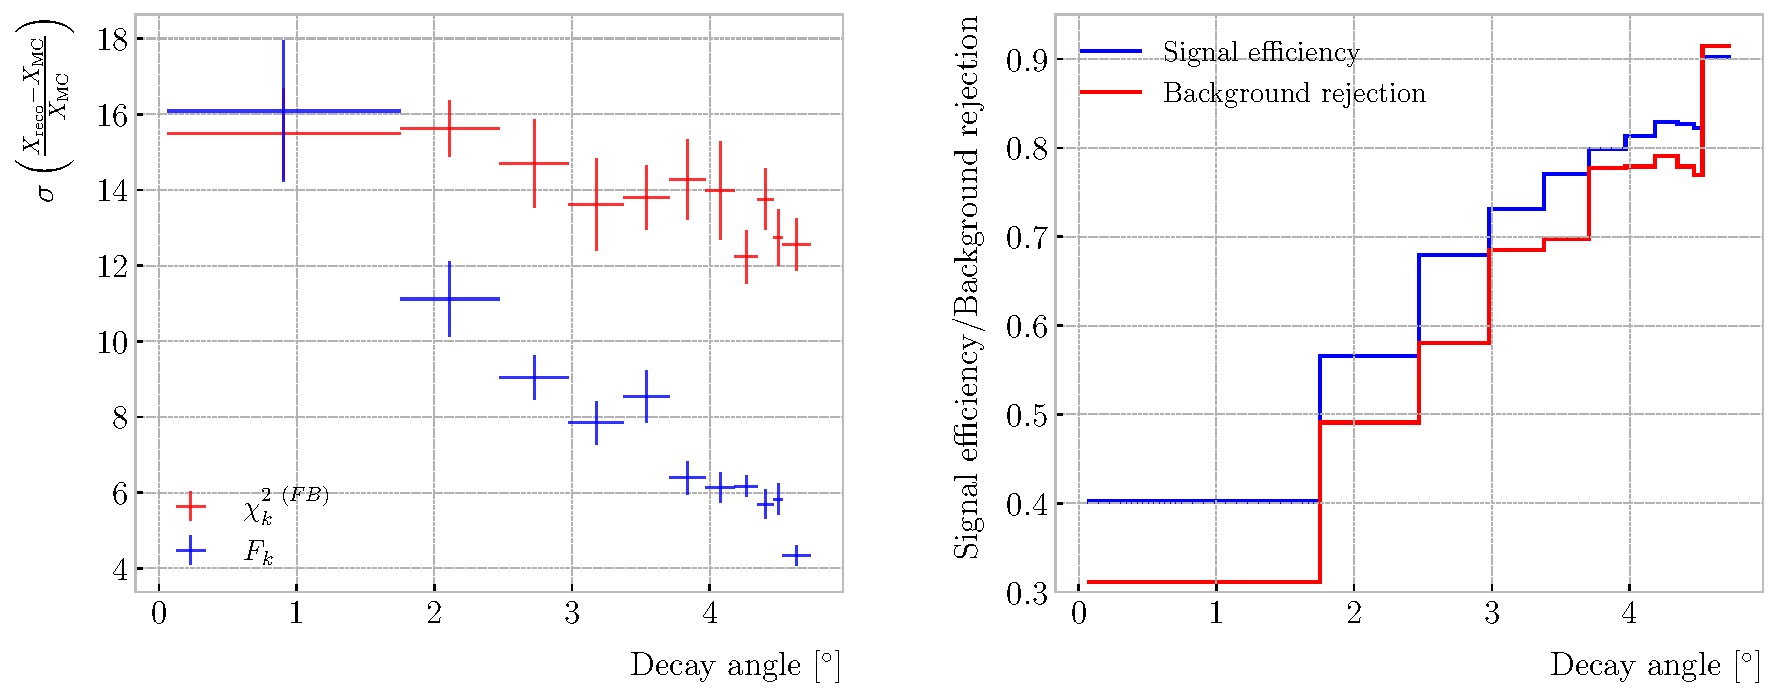
\includegraphics[width=.85\linewidth]{Images/GArSoft_PID/pion_decay/pion_decay_angle_summary2.pdf}
	\caption{Left panel: dependence of the decay position finding resolution on the true value of the decay angle for the $\chi_{k}^{2 \ (FB)}$ (red) and $F_{k}$ (blue) methods. Right panel: signal efficiency (blue line) and background rejection (red line) from the BDT classifier versus true decay angle.}
	\label{fig:breakpoint_angle}
\end{figure}

An approach to this classification could be using a boosted decision tree (BDT). One of the advantages of BDTs is that they are easy to interpret and identify the relative importance of the different input variables. Training a BDT with $400$ estimators and a maximum depth of $4$ I can obtain an efficient classification without overtraining. Figure \ref{fig:breakpoint_bdt} (left panel) shows the distribution of probabilities predicted by the BDT for a test sample. The signal efficiency as a function of background acceptance, the so-called ROC curve, is shown in Fig. \ref{fig:breakpoint_bdt} (right panel). With a relative importance of $0.83$, the most important variable turned out to be $D_{k}^{1/R \ (min)}$.

One thing we can check is how the resolution to the decay and the signal efficiency in the classification changes with the true decay angle. Using an equal-frequency binning for the decay angles, we can repeat the previous steps for each bin.

Figure \ref{fig:breakpoint_angle} (left panel) shows the dependence on the decay angle of the decay finding resolution. We can see that for the $\chi_{k}^{2 \ (FB)}$ maximum location method the resolution consistently lies between $12$ to $16\%$. However, the $F^{(max)}_{k}$ approach gives a significantly better resolution for high angle values, reaching the $4-6\%$ range for decay angles $\geq 4^{\circ}$.

For the classification dependence on the angle, I use the same classifier I trained before but evaluating the test sample for each individual angular bin. I compute the signal efficiency in each bin for a fixed value of the background rejection, in this case $90\%$. Similarly, for the background rejection estimation I use a fixed signal efficiency value of $90\%$. Figure \ref{fig:breakpoint_angle} (right panel) represents the change in signal efficiency (blue) and background rejection (red) with the value of the true decay angles.

\section{Neutral particle identification}\label{section:neutral}

\subsection{ECal clustering}

Another important reconstruction item is the clustering algorithm of ECal hits in GArSoft. The default module features a NN algorithm that treats all hits in the same way, independently of the layer each hit comes from. However, the current ECal design of ND-GAr has two very different types of scintillator layers. The inner layers are made out of tiles, which provide excellent angular and timing resolutions. On the other hand, the outer layers are cross scintillator strips. That way, an algorithm that treats hits from both kinds of layers differently may be able to improve the current performance.

Inspired by the reconstruction of T2K's ND280 downstream ECal \cite{T2KUK2013}, the idea was to put together a clustering module that first builds clusters for the different ECal views (tiles, strips segmented in the $X$ direction and strips segmented in $Y$ direction), and then tries to match them together to form the final clusters.

Working on a module-by-module basis, the algorithm first separates the hits depending on the layer type they come from. Then, it performs a NN clustering for the 3 sets of hits separately. For the tile hits it clusters together all the hits which are in nearest-neighbouring tiles and nearest-neighbouring layers, for strip hits it looks at nearest-neighbouring strips and next-to-nearest-neighbouring layers (as the layers with strips along the two directions are alternated). For strip clusters an additional cut in the direction along the strip length is needed.

After this first clustering I then apply a recursive re-clustering for each collection of strip clusters based on a PCA method. In each case, we loop over the clusters with $N_{hits}\geq2$, computing the centre of mass and three principal components. Propagating these axes up to the layers of the rest of the clusters, we check if the propagated point and the centre of mass of the second cluster are within next-to-nearest-neighbouring strips. An additional cut in the direction along the strip length is also needed. Moreover, I require that the two closest hits across the two clusters are at most in next-to-nearest-neighbouring strips. I merge the clusters if these three conditions are satisfied. The re-clustering is repeated until no more cluster pairs pass the cuts.

The clusters in each strip view are combined if their centres of mass are close enough and they point in the same direction. An alternative approach for the strip cluster merging could be to compute the overlap between the ellipsoids defined by the principal axes of the clusters, and then merge the pair if the overlap exceeds some threshold. Further study is needed to understand if this change would have an impact in the overall clustering performance.

To merge the tile clusters to the combined strip clusters I propagate the principal axis of the strip cluster towards the inner layers, up to the centre of mass layer of the tile cluster. I merge the clusters if the distance between the propagated point and the centre of mass is bellow a certain cut.

The last step is to check if clusters in neighbouring modules should be merged together, both across two barrel modules, across end cap modules and between barrel end cap modules. I check the distance between the two closest hits in the pair of clusters and merge them if it passes this and an additional direction cut.

Figure \ref{fig:clustering_example} presents an example of the clustering steps relevant for strip layer hits, from the input hits (top left panel) to the NN clustering (top right panel) and re-clustering (bottom left panel) for each strip view and the final merging strip clusters (bottom right panel). It shows the hits from a single ECal barrel module in a $\nu_{\mu}$ CC interaction event with a neutral pion and a proton in the final state. The two clusters on the left correspond to the photon pair from the $\pi^{0}$ decay and the one on the upper right corner is associated to the proton.

\begin{figure}[t]
	\centering
	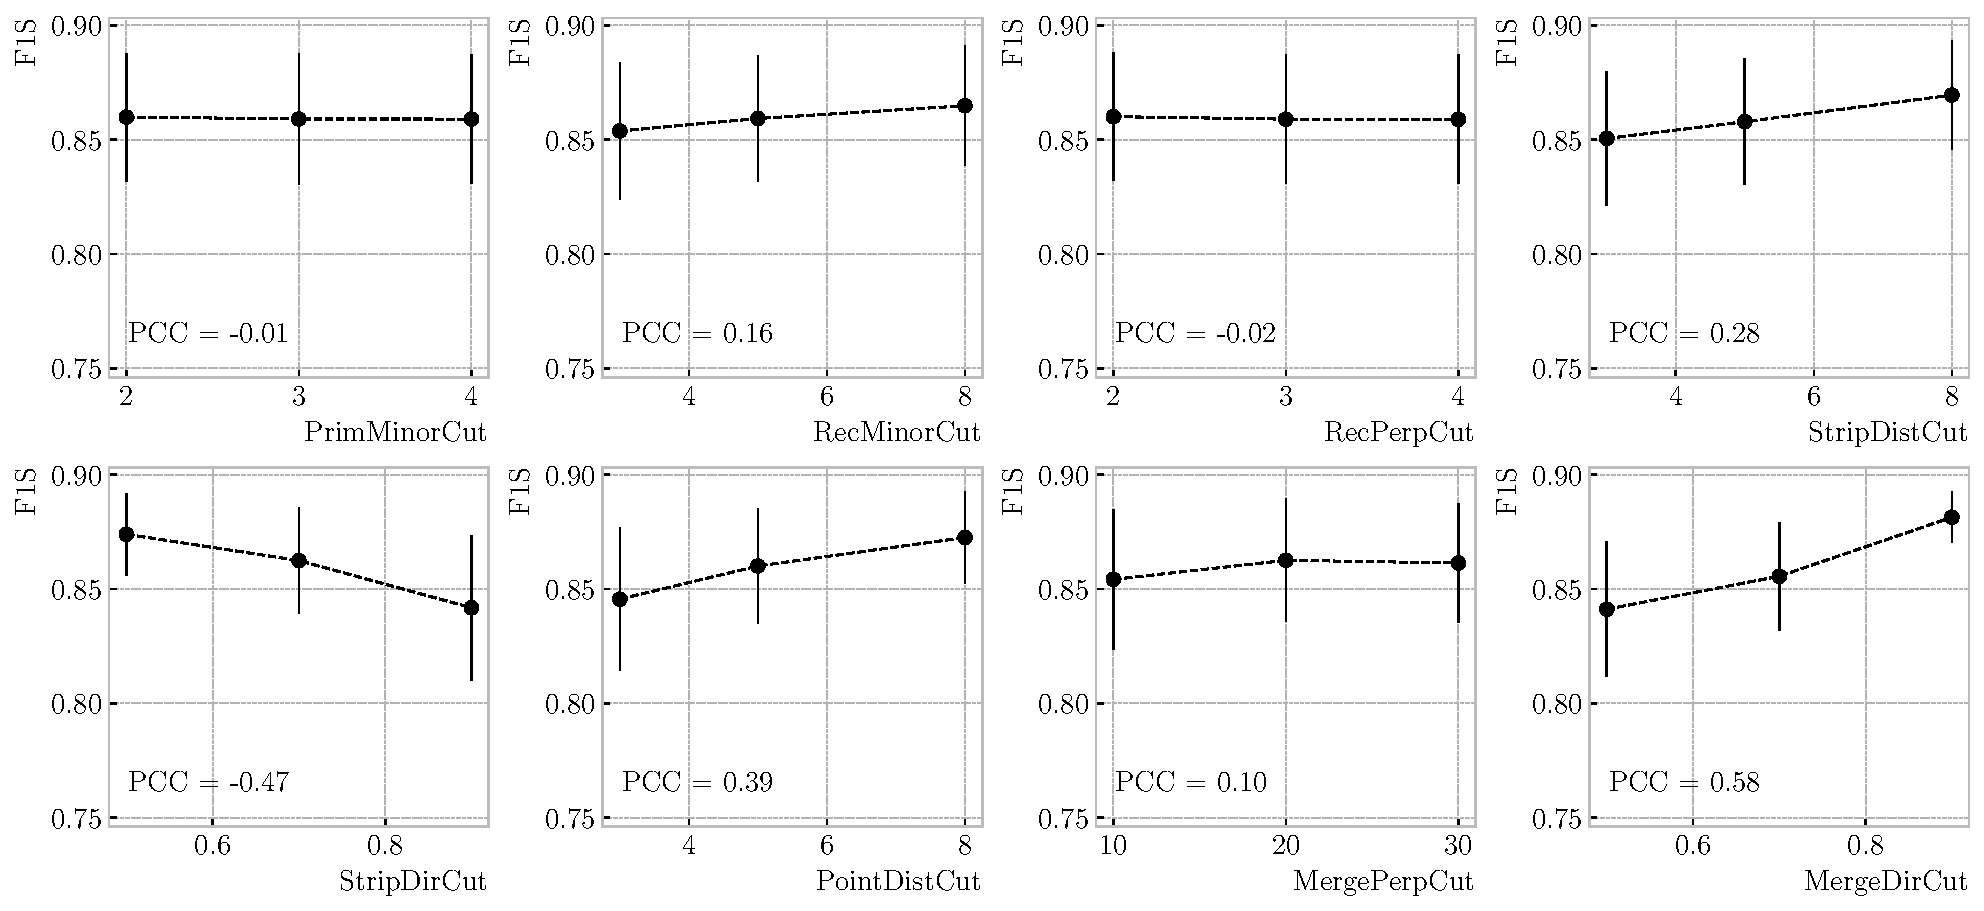
\includegraphics[width=.99\linewidth]{Images/GArSoft_PID/Neutral/coolcluster_optimisation_F1S.pdf}
	\caption{Mean values of the $F_{1}$-score marginal distributions for the different free parameters of the new clustering algorithm, with the error bars representing one standard deviation around the mean. The $F_{1}$-score values were computed for the 6561 possible parameter configurations using 1000 $\nu_{\mu}$ CC interaction events.}
	\label{fig:clustering_optimisation}
\end{figure}

\begin{table}[h!]
	\centering
	\caption{Summary of parameters and sampled values used in the optimisation of the clustering algorithm.}
	\begin{tabular}{l|l|l|p{7cm}}
		Name         & Units  & Sampled values & Description                                                                  \\ \hline
		PrimMinorCut & strips & 2, 3, 4        & Distance along strip length in NN clustering                                 \\
		RecMinorCut  & strips & 3, 5, 8        & Distance between propagated point and CM along strip length in re-clustering \\
		RecPerpCut   & strips & 2, 3, 4        & Closest hit pair distance in re-clustering                                   \\
		StripDistCut & strips & 3, 5, 8        & Distance between CMs in strip cluster merging                                \\
		StripDirCut  & cos    & 0.5, 0.7, 0.9  & Main axes direction cut in strip cluster merging                             \\
		PointDistCut & tiles  & 3, 5, 8        & Distance between propagated point and CM in strip-tile matching              \\
		MergePerpCut & cm     & 10, 20, 30     & Closest hit pair distance in module merging                                  \\
		MergeDirCut  & cos    & 0.5, 0.7, 0.9  & Main axes direction cut in module merging                                   
	\end{tabular}
	\label{tab:clustering_optimisation}
\end{table}

This algorithm has a total number of eight free parameters that need to be optimised. I used a sample of 1000 $\nu_{\mu}$ CC interactions in order to obtain the optimal configuration of clustering parameters. This sample was generated up to the default ECal hit clustering level, so then I could run the new clustering algorithm each time with a different configuration of parameters. As the number of parameters is relatively large, I only performed a coarse-grained scan of the parameter space. Sampling each of the eight parameters at three different points each I obtain 6561 different configurations. These parameters, together with the used values, are summarised in Tab. \ref{tab:clustering_optimisation}.

In order to measure the performance of the clustering, I use a binary classification approach. For each formed cluster, I identify the Geant4 Track ID of the matching MC particle and the energy fraction of each hit. Then, I assign to each cluster the Track ID with the highest total energy fraction. For each of the different Track IDs associated to the clusters, I select the cluster with the highest energy (only from the hits with the same Track ID). I identify such a cluster as the main cluster for that Track ID. I count as true positives (TPs) the hits with the correct Track ID in each main cluster. False positives (FPs) are the hits with the incorrect Track ID for the cluster they are in, not only main clusters. The false negatives (FNs) are the hits with the correct Track ID in clusters other than the main.

Figure \ref{fig:clustering_optimisation} shows the computed $F_{1}$-score values for the different cuts. In each case, the central value represents the mean of the $F_{1}$-score distribution for the specified value of the corresponding variable and the vertical error bar represents one standard deviation around the mean. Also shown are the Pearson correlation coefficients of these central values. We can see that five of the variables have a sizeable effect on the $F_{1}$-score, with an absolute difference between the last and first values as big as $4\%$.

The working configuration is obtained as follows. I first select all configurations with purity $\geq90\%$. Among those, I choose the combinations that yield the maximum $F_{1}$-score. If more than one configuration remains I select the one with the highest sensitivity. Doing so, I end up with a parameter configuration with an efficiency of $88\%$ and a $90\%$ purity. Compared with the default algorithm, which gives an efficiency of $76\%$ and a purity of $91\%$ for the same sample, I have managed to improve the efficiency by a factor of $1.16$.

\subsection[\texorpdfstring{$\pi^{0}$}{pi0} reconstruction]{\boldmath\texorpdfstring{$\pi^{0}$}{pi0} reconstruction}

\begin{figure}[t]
	\begin{subfigure}{0.5\textwidth}
		\centering
		\includegraphics[width=.99\linewidth]{Images/GArSoft_PID/Neutral/coolcluster_clusters_per_photon.pdf}
	\end{subfigure}
	\begin{subfigure}{0.5\textwidth}
		\centering
		\includegraphics[width=.99\linewidth]{Images/GArSoft_PID/Neutral/coolcluster_invariant_mass_vertex.pdf}
	\end{subfigure}
	\caption{Left panel: distributions of the number of ECal clusters per photon from $\pi^{0}$ decays for the standard (red) and new (blue) clustering algorithms. Right panel: reconstructed invariant mass distributions for photon pairs from single $\pi^{0}$ events using the standard (red) and new (blue) ECal clustering algorithms.}
	\label{fig:clustering_pizero}
\end{figure}

One of the potential applications of the new ECal hit clustering is the reconstruction of neutral particles, in particular pions. Neutral pions decay promptly after being produced, through the $\pi^{0} \rightarrow \gamma\gamma$ channel $(98.823 \pm 0.034)\%$ of the time. The photon pair does not leave any traces in the HPgTPC (unless one or both of them converts into an electron-positron pair), but each of them will produced an electromagnetic shower in the ECal.

To test the potential impact of the new algorithm in $\pi^{0}$ reconstruction, I generated a MC sample of single, isotropic neutral pions inside the HPgTPC. All pions were generated with a momentum $p = 500 \ \mathrm{MeV}$ and their initial positions were uniformly sampled inside a $2 \times 2 \times 2 \ \mathrm{m}$ box aligned with the centre of the TPC. I ran both the default and the new clustering algorithms, using for the latter the optimised configuration discussed above.

The first thing to notice is that the number of clusters produced per photon has decreased. Figure \ref{fig:clustering_pizero} (left panel) shows these distributions for the default (red) and new (blue) algorithms. Using a simple Gaussian fit, we see that the mean number of ECal clusters per photon went from $1.82 \pm 0.01$ to $1.09 \pm 0.03$. This effectively means that with the new algorithm the ECal activity of one true particle is typically reconstructed as a single object. From the reconstruction point of view this can be an advantage. As now most of the photon energy ends up in a single ECal cluster, I can simply use cluster pairs to identify the $\pi^{0}$ decay.

In general, one calculates the invariant mass of the photon pair as:
\begin{equation}
	m_{\gamma\gamma} = \sqrt{2E_{1}E_{2}(1-\mathrm{cos} \ \theta)},
\end{equation}
where $E_{i}$ are the energies of the photons and $\theta$ the opening angle between them. In this case I can use the energies deposited in the ECal and their incident directions. This quantity is computed for all possible pairs of clusters, using their position together with the true decay point. In a more realistic scenario, e.g. $\nu_{\mu}$ CC interaction, one could use the position of the reconstructed primary vertex instead. I also tried to use the principal direction of the clusters, but that approach gave considerably worse results. For each event I only keep the pair with an invariant mass closer to the true $\pi^{0}$ mass value.

Figure \ref{fig:clustering_pizero} (right panel) shows the invariant mass distributions for the photon pairs we get using the default (red) and the new (blue) ECal clustering algorithms. For the fit I used a modified version of the Crystal Ball function \cite{Gaiser1982}, obtained by taking the limit where the parameter controlling the power-law tail goes to infinity:
\begin{equation}
	f(x; N, \mu, \sigma, \alpha) = N \cdot
	\left\{
	\begin{array}{ll}
		\mathrm{e}^{\frac{\alpha(2x-2\mu+\alpha\sigma)}{2\sigma}};& x \leq \mu - \alpha\sigma,\\
		\mathrm{e}^{-\frac{(x-\mu)^{2}}{2\sigma^{2}}};& x > \mu - \alpha\sigma.
	\end{array}
	\right.
\end{equation}
Comparing the fitted mean and standard deviation values for the Gaussian cores, we see that the distribution for the new algorithm is a $67\%$ narrower and also peaks much closer to the true $m_{\pi^{0}}$ value, going from $101.3 \pm 0.4 \ \mathrm{MeV}$ to $130.8 \pm 0.6 \ \mathrm{MeV}$.

\section{Integration in GArSoft}\label{section:integration}

All the additions and improvements to the reconstruction discussed in this Chapter had to be integrated in the GArSoft framework. This is necessary both to allow a more streamlined path for development, as this makes testing and adding features straightforward, as well as make the changes usable in future productions of simulated data. In this section, I outline the current status of the integration in GArSoft of the reconstruction work presented above.

The new track-cluster association code has been implemented in GArSoft, under the name of \texttt{TPCECALAssociation2}, and has now become the new default in the reconstruction. The structure of the module is similar to the previous implementation, and the data products they output are identical in form. Therefore, any existing code using the association objects does not need to be modified.

\begin{figure}[t]
    \centering
    \includegraphics[width=.99\linewidth]{Images/GArSoft_PID/caf_proton_scores.pdf}
    \caption[Distributions of proton $\mathrm{d}E/\mathrm{d}x$ and ToF scores for a sample of 100000 FHC neutrino interactions in the HPgTPC.]{Distributions of proton $\mathrm{d}E/\mathrm{d}x$ (left panel) and ToF (right panel) scores for a sample of 100000 FHC neutrino interactions in the HPgTPC. The distributions are broken down by the true particle type associated to the reconstructed particle.}
    \label{fig:proton_scores}
\end{figure}

The computation of the truncated mean $\mathrm{d}E/\mathrm{d}x$ of the tracks, the evaluation of the muon score for muon and pion separation, and the estimation of the velocity from time-of-flight are all orchestrated by the \texttt{CreateRecoParticles} module. Each one of these is implemented as a separate algorithm, which is then called by the parent module. This generates the \texttt{gar::rec::RecoParticle} products, a new high-level data object in GArSoft. These combine the information from the HPgTPC, ECal, and $\mu$ID to create an object useful for analysers. At the moment, these data products are only generated for charged particles. However, in the future the module can be extended to incorporate other algorithms used for the identification of neutral particles, like neutral pions and neutrons.

Additionally, analogous to the muon score, the \texttt{gar::rec::RecoParticle} objects contain two other scores based on the $\left<\mathrm{d}E/\mathrm{d}x\right>$ and ToF estimates which measure the ``protoness'' of a reconstructed particle. These are a obtained in a number of momentum bins, and are a measure of the distance to the point in the corresponding distribution that maximises the $F_{1}$-score for the proton separation. This distance is then transformed applying a sigmoid function, which produces a score in the $0-1$ range, with coefficients obtained following a procedure similar to the one used to calibrate the response of the muon score. The $\mathrm{d}E/\mathrm{d}x$ proton score is defined for all particles with momenta $p_{\mathrm{reco}} < 1.5~\mathrm{GeV}/c$, whereas the ToF proton score is available for the particles with at least one associated hit in the inner ECal and momentum in the range $0.5 \leq p_{\mathrm{reco}} < 3.0~\mathrm{GeV}/c$. As an example, Fig. \ref{fig:proton_scores} shows the distributions of the $\mathrm{d}E/\mathrm{d}x$ (left panel) and ToF (right panel) proton scores for the reconstructed particles in a 100000 FHC neutrinos sample.

The calculation of the track breakpoint variables for pion decay identification is currently implemented as an analysis module in GArSoft. It would be interesting to add this information to the \texttt{gar::rec::RecoParticle} products, possibly calling the code as an additional algorithm in the \texttt{CreateRecoParticles} module. However, the best way to propagate the information to the high-level objects is still unclear.

About the new ECal clustering algorithm, it is still in a development phase, and as such it has not replaced the current clustering module. At the moment, its latest version is integrated in GArSoft as the \texttt{CaloClustering2} module. The algorithm used is implemented separately, and then invoked in the main code. The module can be run standalone on the outputs of the reconstruction, creating a second instance of the \texttt{gar::rec::Cluster} collection. In the future it may replace the current algorithm as the default in the reconstruction chain. However, more work is needed in order to understand its performance in all the different use cases.